
\documentclass[12pt,utf8]{article}
%%
% CUMUM Thesis template
% Created by Caibin Zeng, email: macbzeng@scut.edu.cn  %
% July 8, 2022
%%
% 承诺书页和编号专用页,直接在官网Word模板编辑,再转成PDF
% 本模板只涉及正文部分

%% 页面布局 %%
\usepackage{geometry}
\geometry{a4paper,left=2.5cm,right=2.5cm,top=2.5cm,bottom=2.5cm}

%% 必备宏包及说明 %%

% 显示中文
\usepackage{ctex}
% 章节题目居中且第一级编号设置为中文样式
\usepackage{sectsty}
\sectionfont{\centering}
\renewcommand\thesection{\chinese{section}、}
\renewcommand\thesubsection{\arabic{section}.\arabic{subsection}}
% 颜色宏包
\usepackage[dvipsnames]{xcolor}
% 三线表宏包
\usepackage{booktabs}
\usepackage{makecell}
% 数学字体宏包
\usepackage{amsfonts}
% 超链接宏包
\usepackage{hyperref}
\hypersetup{colorlinks,
	linkcolor=red,
	anchorcolor=blue,
	pdfstartview=Fit,
	breaklinks=true}
% 数学公式宏包
\usepackage{amsmath}
% 表格宏包
\usepackage{multirow} 
% 图形宏包
\usepackage{graphicx} 
\usepackage{subcaption}	
\usepackage{float}
% 动画宏包
\usepackage[dvipdfmx]{animate}
%代码宏包
\usepackage{listings}
\lstset{
  frame=tb,
  aboveskip=3mm,
  belowskip=3mm,
  showstringspaces=false,
  columns=flexible,
  framerule=1pt,
  rulecolor=\color{gray!35},
  backgroundcolor=\color{gray!5},
  basicstyle={\small\ttfamily},
  numbers=none,
  numberstyle=\tiny\color{gray},
  keywordstyle=\color{blue},
  commentstyle=\color{dkgreen},
  breaklines=true,
  breakatwhitespace=true,
  tabsize=3,
}
\renewcommand {\lstlistingname}{源程序}

%启用四级标题
\setcounter{secnumdepth}{4}
\setcounter{tocdepth}{4}



\begin{document}


%% 标题页

\begin{center} 
  % 标题
   \zihao{-2}\bfseries\heiti {关于波浪能最大输出功率的建模与研究}
   \vspace{2ex}
   
   \zihao{3}\bfseries\heiti {摘要}
\end{center}


在发展可再生清洁能源的大趋势下,波浪能的利用越来越广为世人关注。海洋内部丰富的资源是一个亟待开发的宝库,其中一种利用海洋能源的方式便是通过波浪能装置解决深远海供能问题。本文针对波浪能装置,基于牛顿运动定律建立浮子-振子运动的微分方程模型,研究波浪能装置能量输出功率与内置阻尼器阻尼系数之间的关系,得出最大平均能量输出功率与对应的最优阻尼系数配置。

针对问题1:首先根据浮子和振子只做垂荡运动,建立一维浮子-振子运动微分方程模型;其次采用龙格库塔方法,得出该微分方程的数值解,并计算出在阻尼系数恒定的情况下浮子与振子的位移与速度关于时间的变化情况。

针对问题2: 在问题1的基础上通过浮子与振子的相对运动关系建立功率计算模型。在阻尼系数为常数的情况下我们采用二次遍历法求解最大平均输出功率与最优储能阻尼系数。结果为当阻尼系数为31120.10N·s/m时输出功率取到最大值298.2580W。在阻尼系数与浮子和振子的相对速度的绝对值的幂成正比的情况下我们采用二次遗传算法求解最大平均输出功率与最优储能阻尼系数。得出最大平均输出功率为300.2583W,对应的比例系数为93644.8967,幂指数为0.5239。

针对问题3:根据浮子和振子只做垂荡和纵摇运动,假设浮子与振子相互作用点o仅在竖直方向上运动,利用非惯性系和惯性力建立浮子—振子运动的四元二阶微分方程模型,采用龙格库塔方法,得出该微分方程的数值解,并计算出在阻尼系数恒定的情况下浮子与振子的位移、角位移、速度、角速度关于时间的变化情况。

针对问题4:在问题3的基础上通过浮子与振子的相对运动关系建立功率计算模型。通过二次遗传算法趋近整个数据区间内的较为精确的局部最优解。在此解的基础上,我们通过绘制三维立体图,得出在初步最优解的附近范围内,更为精确的最优解。结果为当旋转阻尼器阻尼系数为91149.5、直线阻尼器阻尼系数为26999.5时,波浪能装置获得最大平均输出功率644.024W。


\vspace{2ex}

\noindent{\heiti 关键词:} 牛顿运动定律; 遗传算法;龙格库塔算法;多变量二阶常微分方程; 非惯性参考系

%\begin{figure}[H]
%\centering
%\begin{subfigure}{0.45\textwidth}
%    \includegraphics[width=\textwidth]{./figures/SCUTMM}
%    \caption{华工数模微信公众号}
%\end{subfigure}
%\hfill
%\begin{subfigure}{0.45\textwidth}
%    \includegraphics[width=\textwidth]{./figures/SCUTMM2}
%    \caption*{华工数模QQ群}
%\end{subfigure}
%\end{figure}
%
%\begin{center}
%  \href{http://scut.fanya.chaoxing.com/portal}{\zihao{-2}《数学建模方法概论》慕课平台}
%\end{center}


\clearpage

% chap 1
\section{问题背景与重述}

\subsection{问题背景}

自从人类进入工业时代,传统化石能源的使用对自然生态环境造成了巨大的伤害,发展更加清洁的能源逐步成为了全体人类的共识。海洋作为一个储量丰富的清洁能源库,得到了越来越多的科学家的关注。2021年的一篇来自国家海洋技术中心的报告指出[1]:波浪能技术在海洋领域应用十分广泛,是有望解决深远海供能的一种最有效途径。

PTO是一种简易的波浪能装置。其组成结构如图所示。本篇文章将围绕该类型波浪能装置建立浮子-振子物理模型以描述该体系在特定环境中的运动状态,并基于模型计算最大输出功率与相应的最佳阻尼系数。

   
\subsection{问题重述}
   问题一和问题二主要探讨浮子\textsf{仅做垂荡运动}的情况。其中问题一着重探讨\textit{特定阻尼情况下的浮子-振子物理系统的垂荡位移与速度};问题二基于问题一的模型在直线阻尼器的特定阻尼系数范围内对浮子-振子物理系统中的输出功率进行优化,\textit{寻找最大输出功率与相应的最佳阻尼系数。}
   
   问题三和问题四主要探讨浮子\textsf{同时进行垂荡和纵摇运动}的情况。其中问题三着重探讨\textit{浮子-振子物理系统的垂荡位移,速度,纵摇角位移与角速度}。问题四基于问题三的模型在直线阻尼器和旋转阻尼器的特定阻尼系数范围内\textit{寻找浮子-振子物理系统最大输出功率与相应的最佳阻尼系数。}

% chap 2
\section{问题分析}
四个小问可以将前两问划归一组,后两问划归一组。前两问中需要建立波浪能装置仅做垂荡运动的物理模型,计算特定时刻物理系统的状态,并对输出功率和阻尼系数进行优化;后两问中加入了纵摇运动,对物理模型提出了更高的要求,但求解的内容与前两问大同小异(多出了转动量)。

\textbf{我们的建模思路是:}
\begin{enumerate}
	\item 通过刻画物理系统的动力学状态获得微分方程组;
	\item 基于matlab方法求解微分方程组预测物理模型特定时刻的状态;
	\item 结合物理系统结构与功能输出原理计算优化目标表达式;
	\item 基于matlab方法对优化目标进行优化;
\end{enumerate}

\subsection{问题1的分析}
波浪能装置的垂荡运动是一个较为复杂的运动,在实际计算时我们根据题设条件对模型进行简化。为了方便后续建模,我们将采用非惯性系进行讨论(计算相对位移更加方便)。通过运用牛顿运动定律,我们可以得到二元二阶微分方程组,并使用龙格库塔法进行求解得到结果。模型建立的重点在于选择合适的参考系;难点在于正确的受力分析,尤其需要注意惯性力的数量与方向。

\subsection{问题2的分析}
问题二的物理情境与问题一基本相同,不需要另行建模。根据波浪能装置的结构与功能输出原理,我们不难列出输出功率的积分表达式。当阻尼系数为恒定值时,我们发现常规遍历算法可以通过粗糙计算-精细计算二级方法在可接受的复杂度内得到效果最好的结果;当阻尼系数变化时,遍历法的复杂度变得无法接受,我们选用遗传算法对目标函数进行优化。

\subsection{问题3的分析}
问题三将纵摇运动引入了分析框架,模型复杂度骤升。我们选择将浮子与振子分别分析,将平动与转动分别分析,得到了四元二阶微分方程组。由于问题三所求内容与问题一类似,故我们使用与问题一基本相同的求解方法,在此不重复叙述。

\subsection{问题4的分析}
问题四的物理情境与问题三基本相同,不需要另行建模。问题四所求内容与问题二第二小问类似,故我们采用与问题二第二小问基本相同的求解方法,在此不重复叙述。



% chap 3
\section{模型假设}

为了清晰表达模型的主要思想,我们做出如下假设:
\begin{enumerate}
	\item 假设波浪能装置处于无粘性不可压缩的理想液体(海水)中;
	\item 假设波浪能装置所处环境是无旋的,且无其他特殊扰动;
	\item 假设与波浪能装置相互作用的波浪是微幅规则波,即波长远大于波高;
	\item 假设波浪能装置中的中轴、底座、隔层、PTO的质量可以忽略不计;
	\item 假设波浪能装置内部各处光滑无摩擦;
	\item 假设浮子与振子的质量分布均匀,运动过程中无磨损;
	\item 假设在运动过程中浮子与振子连接处o点仅沿竖直方向运动;
	\item 假设浮子圆柱壳体、圆锥壳体和振子圆柱壳体的厚度均可忽略不计;
	\item 假设浮子在与水面呈一定角度时所受的静水恢复力可以等价为浮子与水面呈90度同等排水体积下的净水恢复力;
	
\end{enumerate}
% chap 4
\section{符号说明}

\begin{table}[h]
	\centering
	\begin{tabular}{p{2cm}<{\centering}p{8cm}<{\centering}p{3cm}<{\centering}}
		\toprule
		符号 & 说明 & 单位 \\
		\midrule
		$\alpha$ & 浮子角位移  & 弧度   \\
		$\dot{\alpha}$ & 浮子角速度 & 弧度/秒 \\
		$\ddot{\alpha}$ & 浮子角加速度 & 弧度/秒$^2$  \\
		$L$ & 波浪激励力力矩振幅 &  牛顿$\cdot$米 \\
		$K_1$ & 扭转弹簧刚度 & 牛顿/米 \\
		$K_2$ & 旋转阻尼器阻尼系数 & 牛顿·秒/米 \\
		$I_a$ & 纵摇附加转动惯量 & 千克·米$^2$ \\
		$I_1$ & 浮子相对o轴转动惯量(o轴垂直纸面) &  千克·米$^2$ \\
		$\theta$ & 振子相对浮子角位移 & 弧度 \\
		$r$ & 振子相对浮子的径向位移 & 米 \\
		$M_2$ & 振子质量 & 千克\\ 
		$x$ & 浮子位移 & 米 \\
		$I_2$ & 振子相对o轴的转动惯量 & 千克·米$^2$ \\
		$\rho$ & 海水密度 & 千克/米$^3$ \\
		$g$ & 重力加速度 & 米/秒$^2$ \\
		$C_{rd}$ & 垂荡兴波阻尼系数  & 牛顿·秒/米 \\
		$f$ & 波浪激励力振幅 & 牛顿 \\
		$K_T$ & 弹簧刚度 &  牛顿/米 \\
		$L_0$ & 弹簧原长 & 米 \\
		$M_a$ & 垂荡附加质量 & 千克 \\
		$M_1$ & 浮子质量 & 千克 \\
		$K_z$ & 直线阻尼器阻尼系数 & 牛顿·秒/米 \\ 
		$R_1$ & 浮子半径 & 米 \\
		\bottomrule
	\end{tabular}
\end{table}




% chap 5
\section{模型的建立与求解}

\subsection{问题1模型的建立与求解}
\subsubsection{模型的建立}
首先,我们对波浪能装置进行受力分析。当波浪能装置静止在水面上时,系统中浮子受到重力与浮力作用,且两个力构成平衡力;系统中振子连接弹簧与阻尼器,同浮子一样处于平衡状态。经过计算,当水面浸没到距离波浪能装置中圆柱体底面以上两米时,系统处于如上所述的平衡状态。为了表述浮子的运动情况,我们在波浪能装置的外部空间中取平衡状态水平面任意一点为原点,竖直向上建立ox轴;为了表达振子运动情况,我们取波浪能装置上圆柱体底面上任意一点为原点,竖直向上建立oy轴。不难发现,ox轴与地球参考系相对静止,oy轴与波浪能装置参考系相对静止。

\begin{figure}[h]
	\centering
	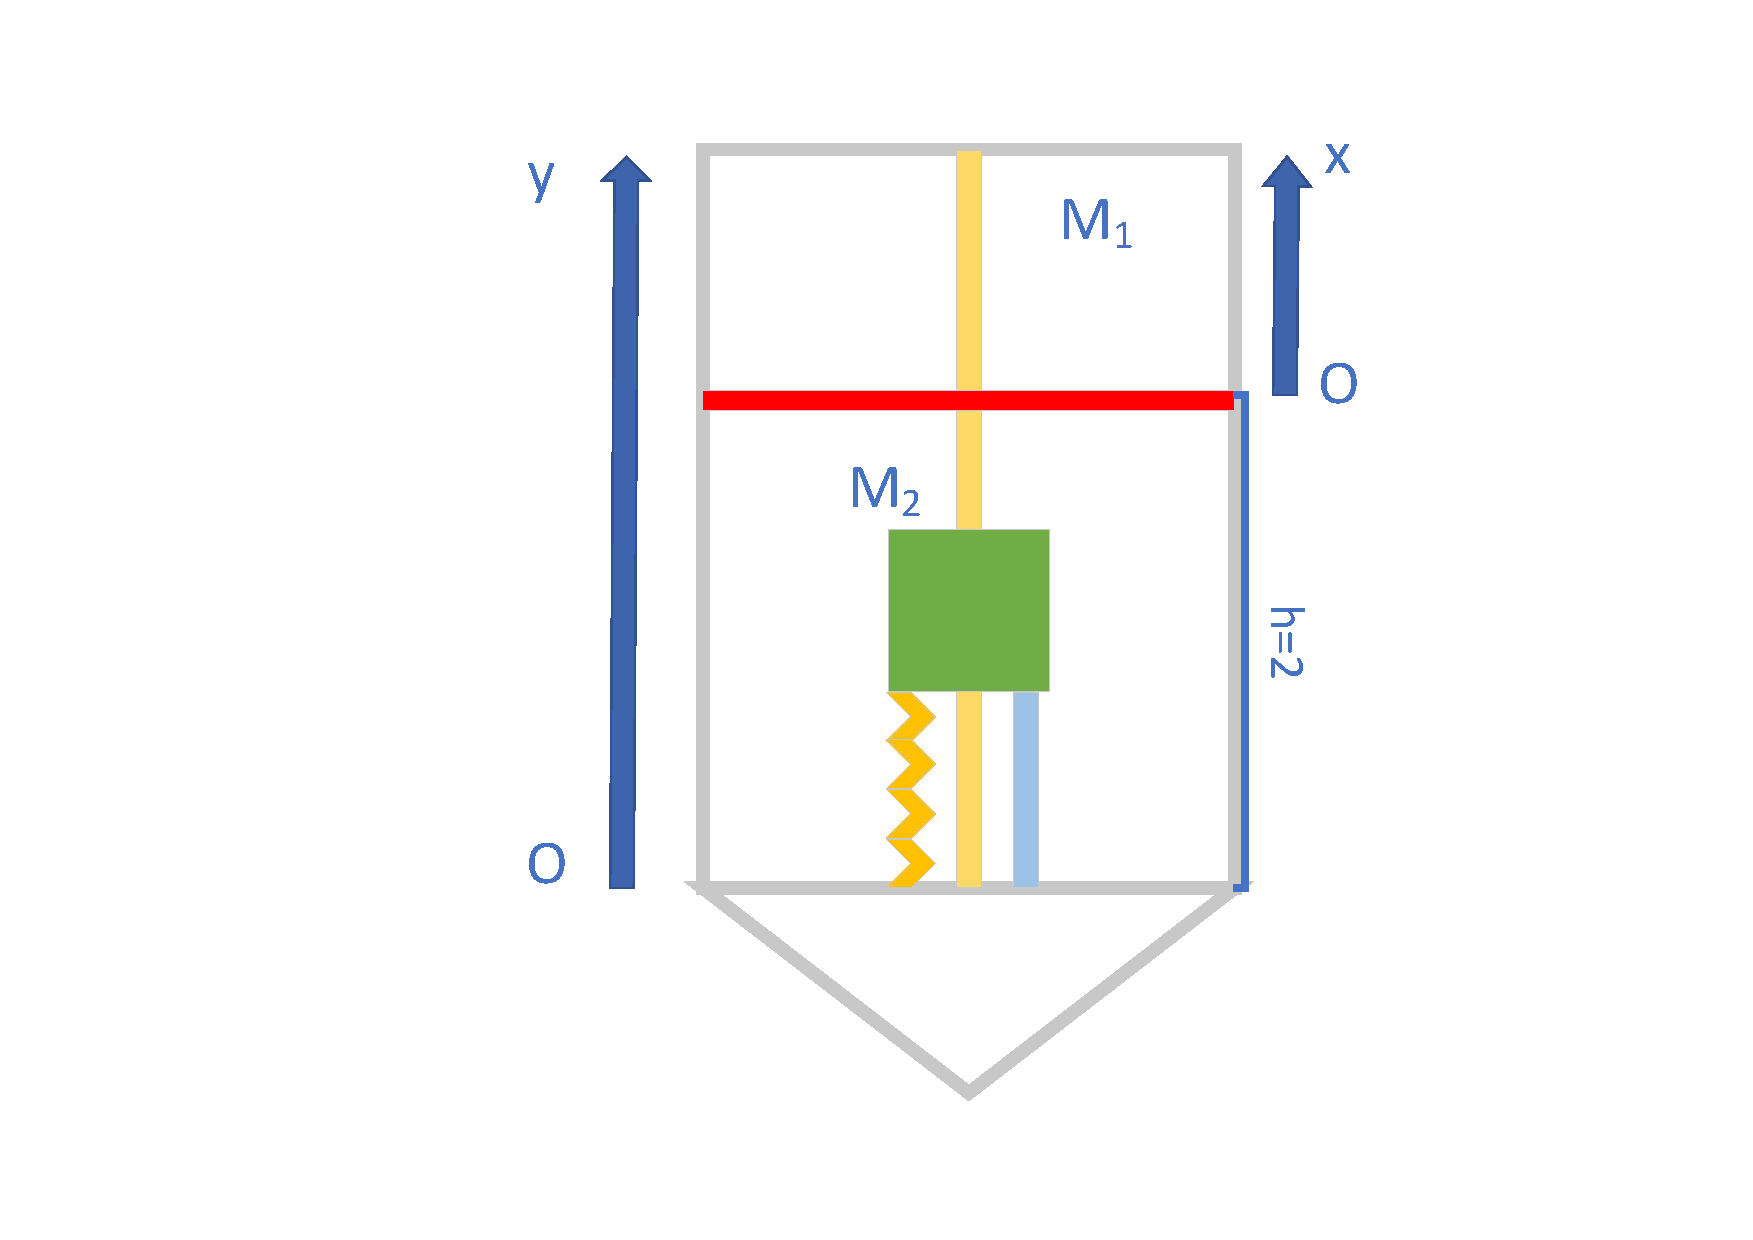
\includegraphics[width=0.4\linewidth]{figures/初态受力分析}
	\caption{波浪能装置初态受力分析}
	\label{图2}
\end{figure}


在问题一中,波浪能装置仅做垂荡运动。在垂荡运动过程中,系统中浮子受力情况可以分为两个部分,即海水对波浪能装置的力与弹簧和直线阻尼器对浮子的作用力。根据牛顿第二定律,浮子的运动方程为:

\begin{equation}
	M_{1} \ddot{x} = f_{h} + F_{z}
\end{equation}

式中 $M_1$ 为浮子质量,x为浮子在ox轴上的位移,$f_h$ 为海水对波浪能装置的作用, $F_z$ 为弹簧和直线阻尼器对浮子的作用力。

具体而言, $f_h$ 有三个组成部分:

\begin{equation}
	f_h = f_b + f_r + f_\epsilon
\end{equation}

式中 $f_b$ 为液体对波浪能装置的静水恢复力, $f_r$ 为附加惯性力与兴波阻尼力的合力, $f_\epsilon$ 为波浪激荡力。这三项的具体表示形式为:

\begin{equation}
	\begin{cases}
		f_b = \rho g \Delta V(x) = - \rho g \pi x R^2 \\
		f_r = -M_a \ddot{x_1}-C_{rd} \dot{x_1} \\
		f_\epsilon = f \cos \omega t
	\end{cases}
\end{equation}

式中 $\rho$为液体密度,$g$ 为重力加速度,$V$为体积函数,$x$为ox轴上波浪能装置下沉或上浮距离,$M_a$表示附加质量,$C_{rd}$表示辐射阻尼系数,$f$为波浪激励振幅,$\omega$为波浪频率[2]与浮子运动方程类似地,我们也可以对振子应用牛顿第二定律求解运动学方程:

\begin{equation}
	M_2 \ddot{y} = f_T + f_z + f_{\text{惯}} - M_2 g
\end{equation}

式中$M_2$为振子质量,$y$为振子在oy轴上的位移,$f_t$为弹簧对振子的作用,$f_z$为阻尼对振子的作用,$ f_{\text{惯}}$为惯性力(oy为非惯性参考系,需要加入惯性力)。$f_t$, $f_z$, $ f_{\text{惯}}$的具体表示形式为:

\begin{equation}
	\begin{cases}
		f_T = -K_T(y-L) \\
		f_z = -K_z \dot{y} \\
		f_{\text{惯}} = -M_2 \ddot{x}
	\end{cases}
\end{equation}

式中$K_T$ 为弹簧弹性系数,$K_z$ 为阻尼系数。

由相互作用关系(牛顿第三定律),我们不难得出先前浮子运动学方程中振子对浮子的作用力$F_z$为:
\begin{equation}
	F_z = -f_T - f_z
\end{equation} 

综上,我们可以如图三表示起振后浮子与振子的受力情况,并列出如下二元二阶微分方程:

\begin{figure}[htbp]
	\centering
	\subfloat[浮子受力分析图]{
		\label{fig:improved_subfig_a}
		\begin{minipage}[t]{0.4\textwidth}
			\centering
			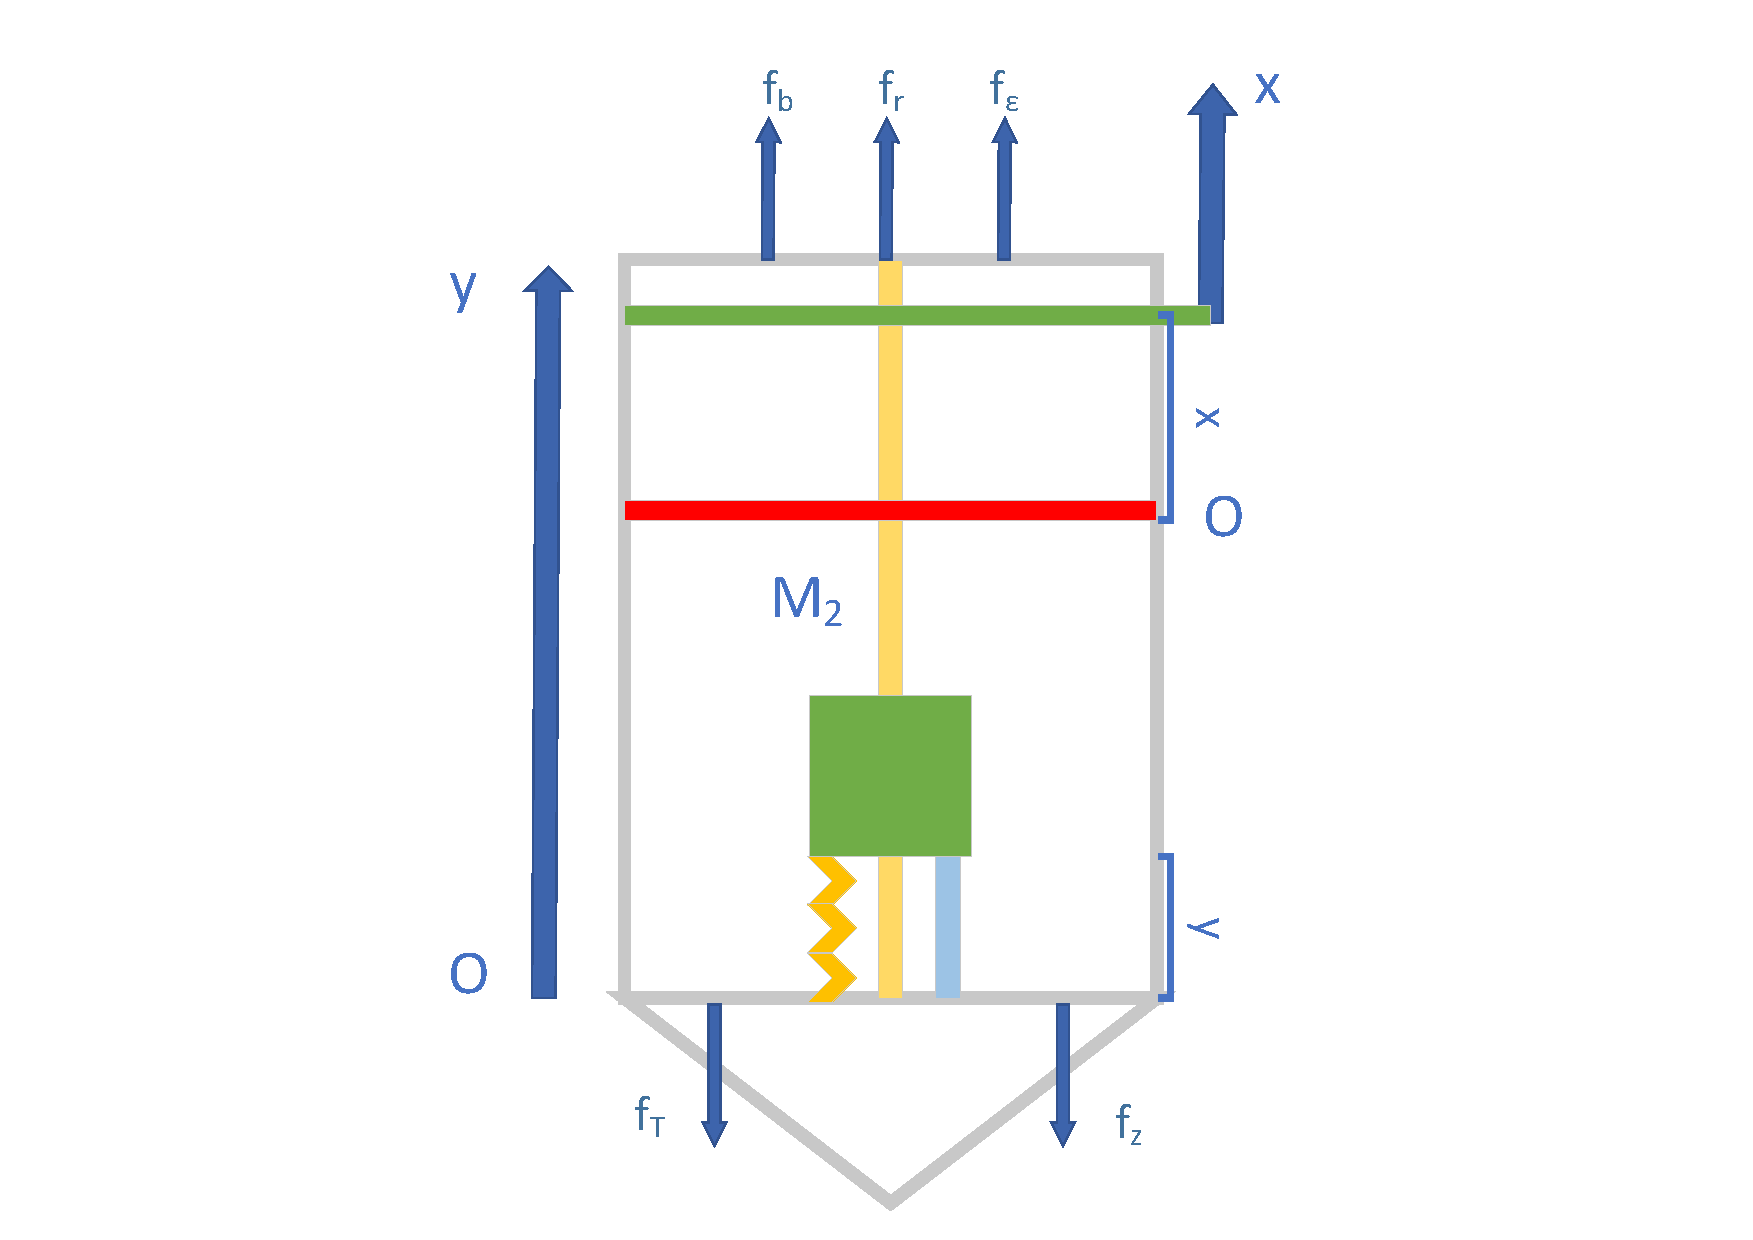
\includegraphics[width=0.6\linewidth]{figures/Q1对浮子受力分析.pdf}
		\end{minipage}
	}
	\subfloat[振子受力分析图]{
		\label{fig:improved_subfig_b}
		\begin{minipage}[t]{0.4\textwidth}
			\centering
			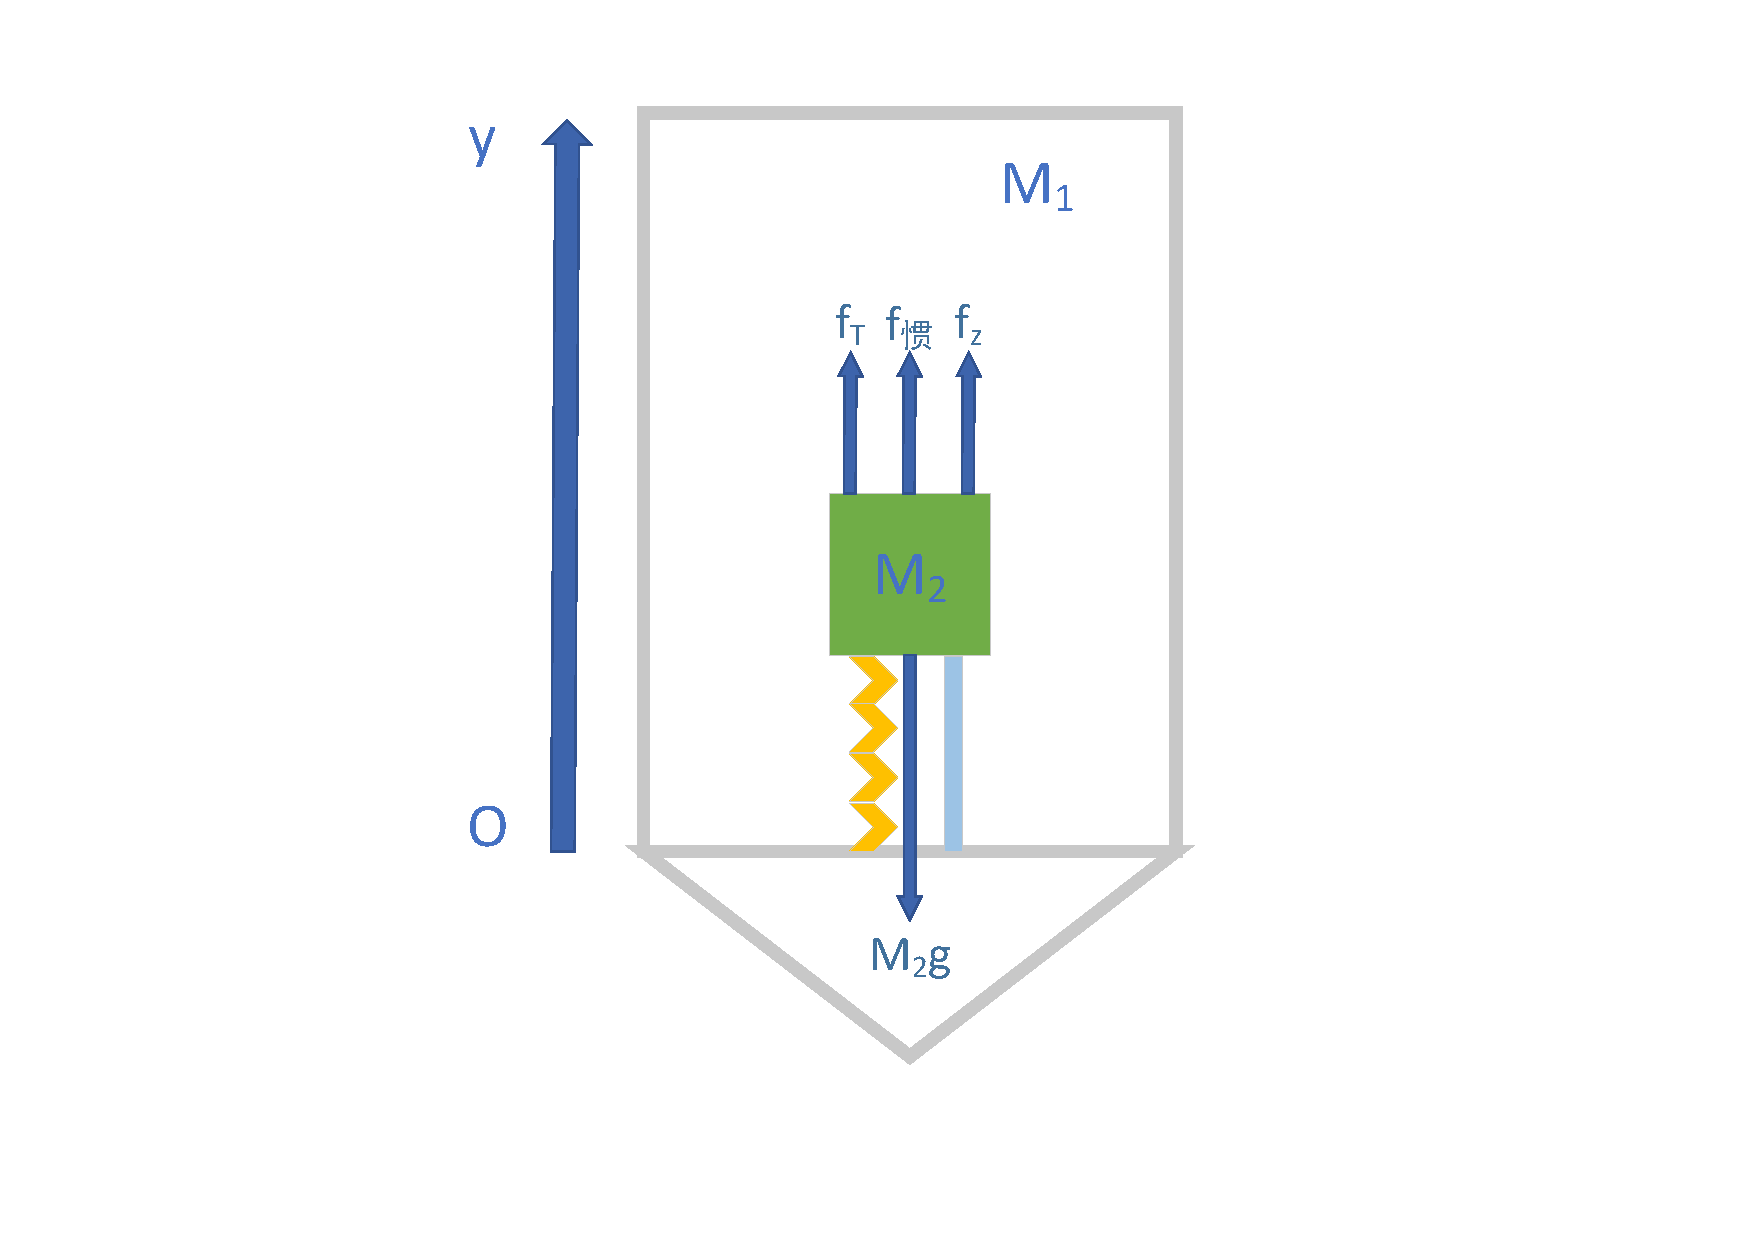
\includegraphics[width=0.6\linewidth]{figures/Q1对振子受力分析.pdf}
		\end{minipage}
	}
	\caption{起振后物理系统受力分析示意图}
\end{figure}


\begin{equation}
	\begin{cases}
		\text{对浮子:}M_1 \ddot{x} = - \rho g \pi x - M_a\ddot{x} - C_{rd}\dot{x} + f\cos (\omega t)  + K_T(y-L)+K_z \dot{y} \\
		\text{对振子:}M_2 \ddot{y} = -K_T (y-L)-K_z\dot{y}-M_2\ddot{x}-M_2 g
	\end{cases}
\end{equation}

通过求解如上二元二阶微分方程,我们最终可以得到浮子位移x(t)和振子位移x(t)+y(t)-2,并通过求导得出浮子与振子的速度。振子位移中-2项来源于ox轴与oy轴初态时相差的距离。

对于问题一的第一小问,题目给出的阻尼系数为$100N\cdot s/m$,与位移呈现线性关系,故不需要改变原二元二阶微分方程。对于问题一的第二小问,由于题设条件发生变更“直线阻尼器的阻尼系数与浮子和振子的相对速度的绝对值的幂成正比,其中比例系数取 10000,幂指数取 0.5”,故应当修改方程组为如下形式:

\begin{equation}
	\begin{cases}
		\text{对浮子:}M_1 \ddot{x} = - \rho g \pi x - M_a\ddot{x} - C_{rd}\dot{x} + f\cos (\omega t)  + K_T(y-L)+K_z |\dot{y}|^{\frac{1}{2}} \dot{y} \\
		\text{对振子:}M_2 \ddot{y} = -K_T (y-L)-K_z|\dot{y}|^{\frac{1}{2}} \dot{y}-M_2\ddot{x}-M_2 g
	\end{cases}
\end{equation}

\subsubsection{模型的求解}

龙格库塔法是一种求解微分方程的常用高精度单步算法,在求解问题一的模型时我们将广泛地使用这种算法。

首先,我们简单回顾龙格库塔算法的原理。龙格库塔算法类似欧拉法,两者都使用过某点$(x_k,y_k)$来近似下一点的函数值$y(x_{k+1})$。欧拉法的缺陷在于它直接使用点$(x_k,y_k)$处切线的斜率$\dot(y(x_k))$近似,因此除非所近似目标为直线,对于$y(x_{k+1})$的求解总是存在一定的误差。

为了解决这一问题,聪明的数学家使用了拉格朗日中值定理。在$(x_k,x_{k+1})$区间内存在一点$\epsilon (x_k < \epsilon < x_{k+1})$,使得等式$f(x_{k+1})-f(x_k) = \dot{f(\epsilon)}(x_{k+1}-x_k)$成立。综上,置信度更高的拟合方程为:

$$
\begin{aligned}
	y(x)&=y(x_k)+\dot{y(\epsilon)}(x-x_k) \\
	&=y(x_k)+\dot{y(x_k+\alpha h)}(x-x_k)
\end{aligned}
$$

当我们等距取值时$(x_{k+1}-x_k = h)$,上述公式可以获得更加直观的形式:

$$
	y(x_{k+1}) = y(x_k)+\dot{y(x_k+\alpha h)}\cdot h
$$

一般的n阶龙格库塔法形式为:

\begin{equation*}
	\begin{cases}
		y_{k+1} = y_k+(\lambda_1 K_1 + \lambda_2 K_2+ \dots +\lambda_n K_n)\cdot h \\
		K_1 = f(x_k,y_k) \\
		K_2 = f(x_k+\alpha_1,y_k+\alpha_1 h K_1) \\
		K_3 = f(x_k+\alpha_2,y_k+\alpha_1 h K_1 + (\alpha_2 - \alpha_1)h K_2) \\
		\vdots \\
		K_n = f(x_k+\alpha_n,y_k+\alpha_1 h K_1 + (\alpha_2 - \alpha_1)h K_2+\dots +(\alpha_n - \alpha_{n-1}h K_{n-1}))
	\end{cases}
\end{equation*}
式中$\lambda$为对应采样点的斜率权值,满足条件$\lambda_1+\lambda_2+\dots +\lambda_n = 1$;$\alpha$为采样点位置比率,满足条件$0<\alpha_1<\alpha_2<\dots<\alpha_n$;h为单步计算长度。在大多数情况下,四阶龙格库塔算法可以得到微分方程拟合效果较好的数值解。

本题我们选择使用matlab中的ode45方法进行求解,该方法使用了四阶龙格库塔方法计算候选解,并用五阶龙格库塔方法控制误差。

经过计算,我们得出问题一的第一小问(阻尼系数恒定)中浮子与振子在10s、20s、40s、60s、100s时的垂荡位移与速度如下。详细结果请参考“支撑材料”文件夹->“T1-1”文件夹->result1-1.xlsx。

\begin{figure}[h]
	\centering
	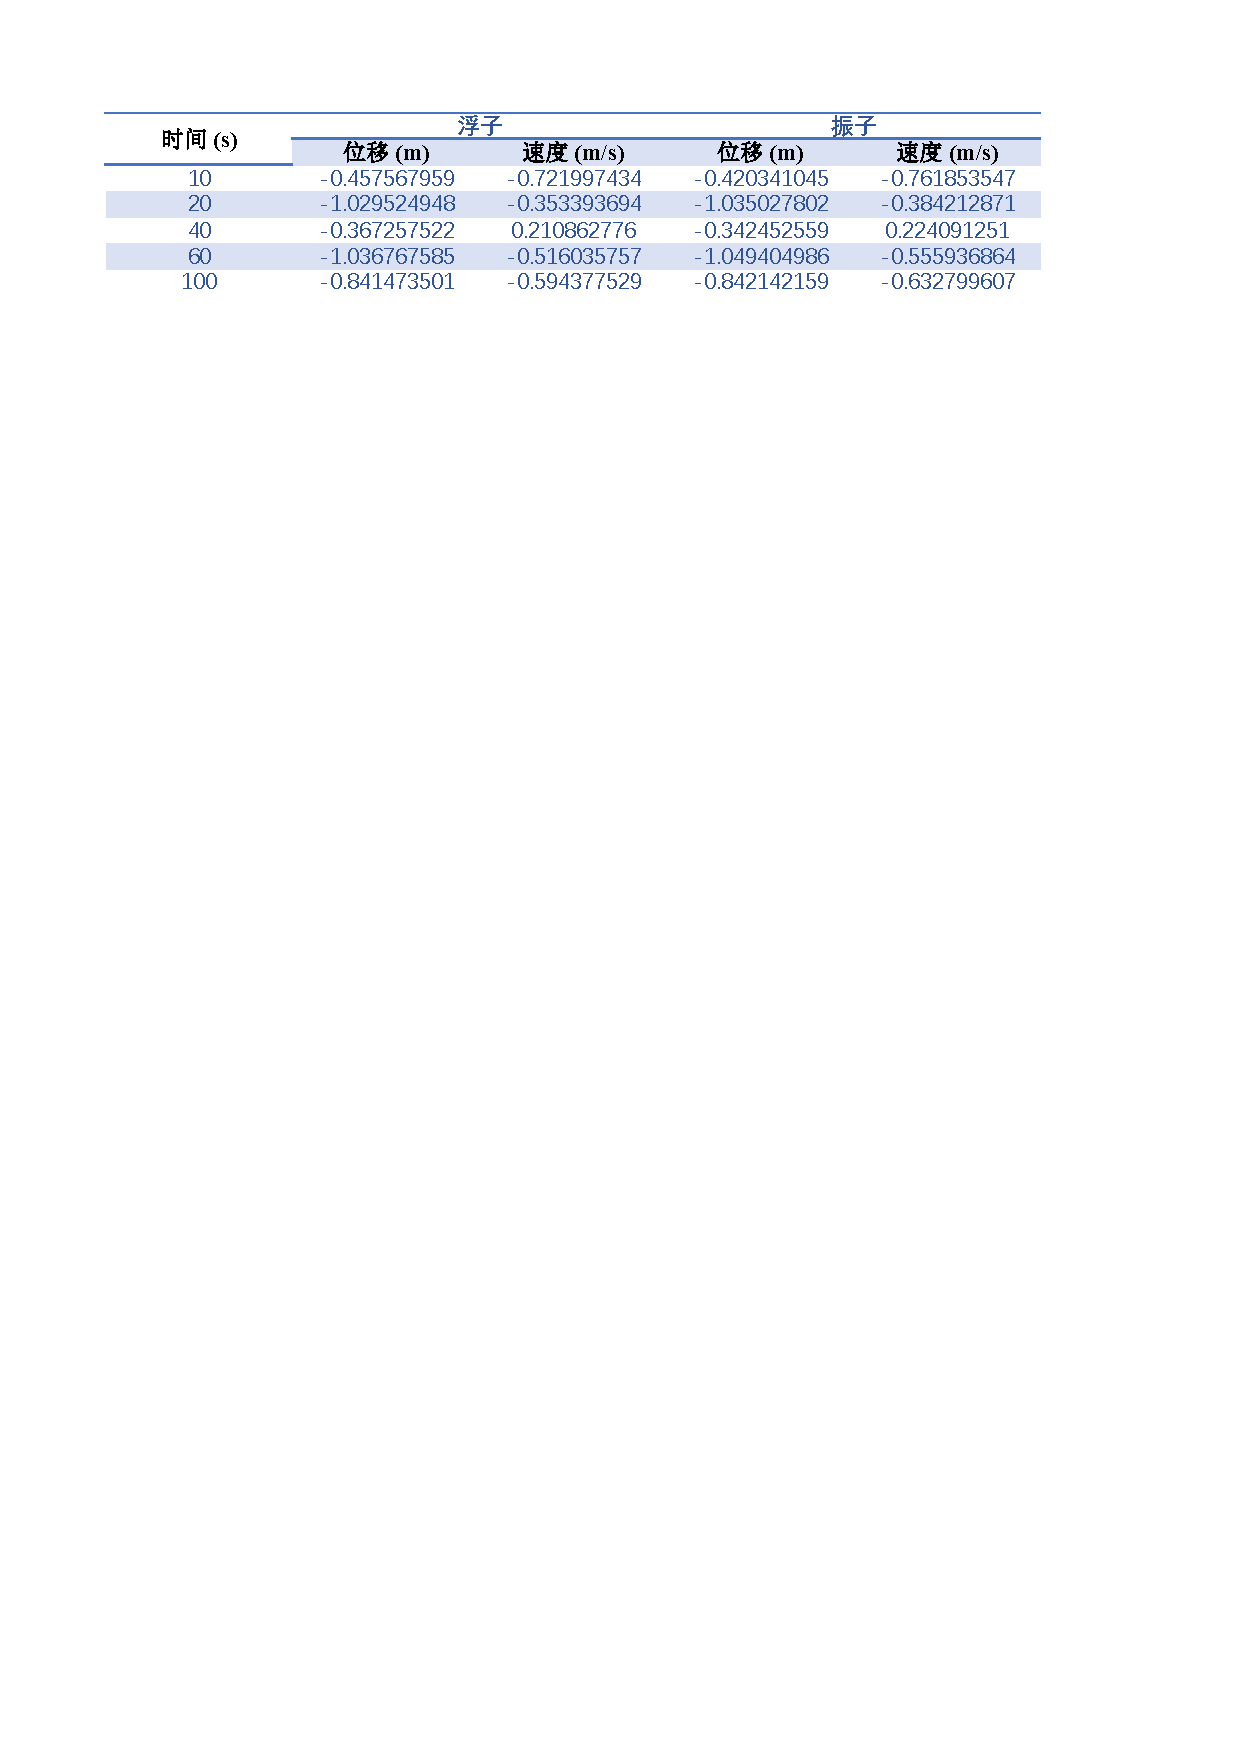
\includegraphics[width=0.7\linewidth]{figures/result1-1}
	\caption[]{阻尼系数恒定时模型计算结果}
	\label{fig:result1-1}
\end{figure}

使用相似的方法,我们也可以计算出问题一的第二小问(阻尼系数变化)中幅值与振子在10s、20s、40s、60s、100s时的垂荡位移。详细结果请参考“支撑材料”文件夹->“T1-2”文件夹->result1-2.xlsx。

\begin{figure}[h]
	\centering
	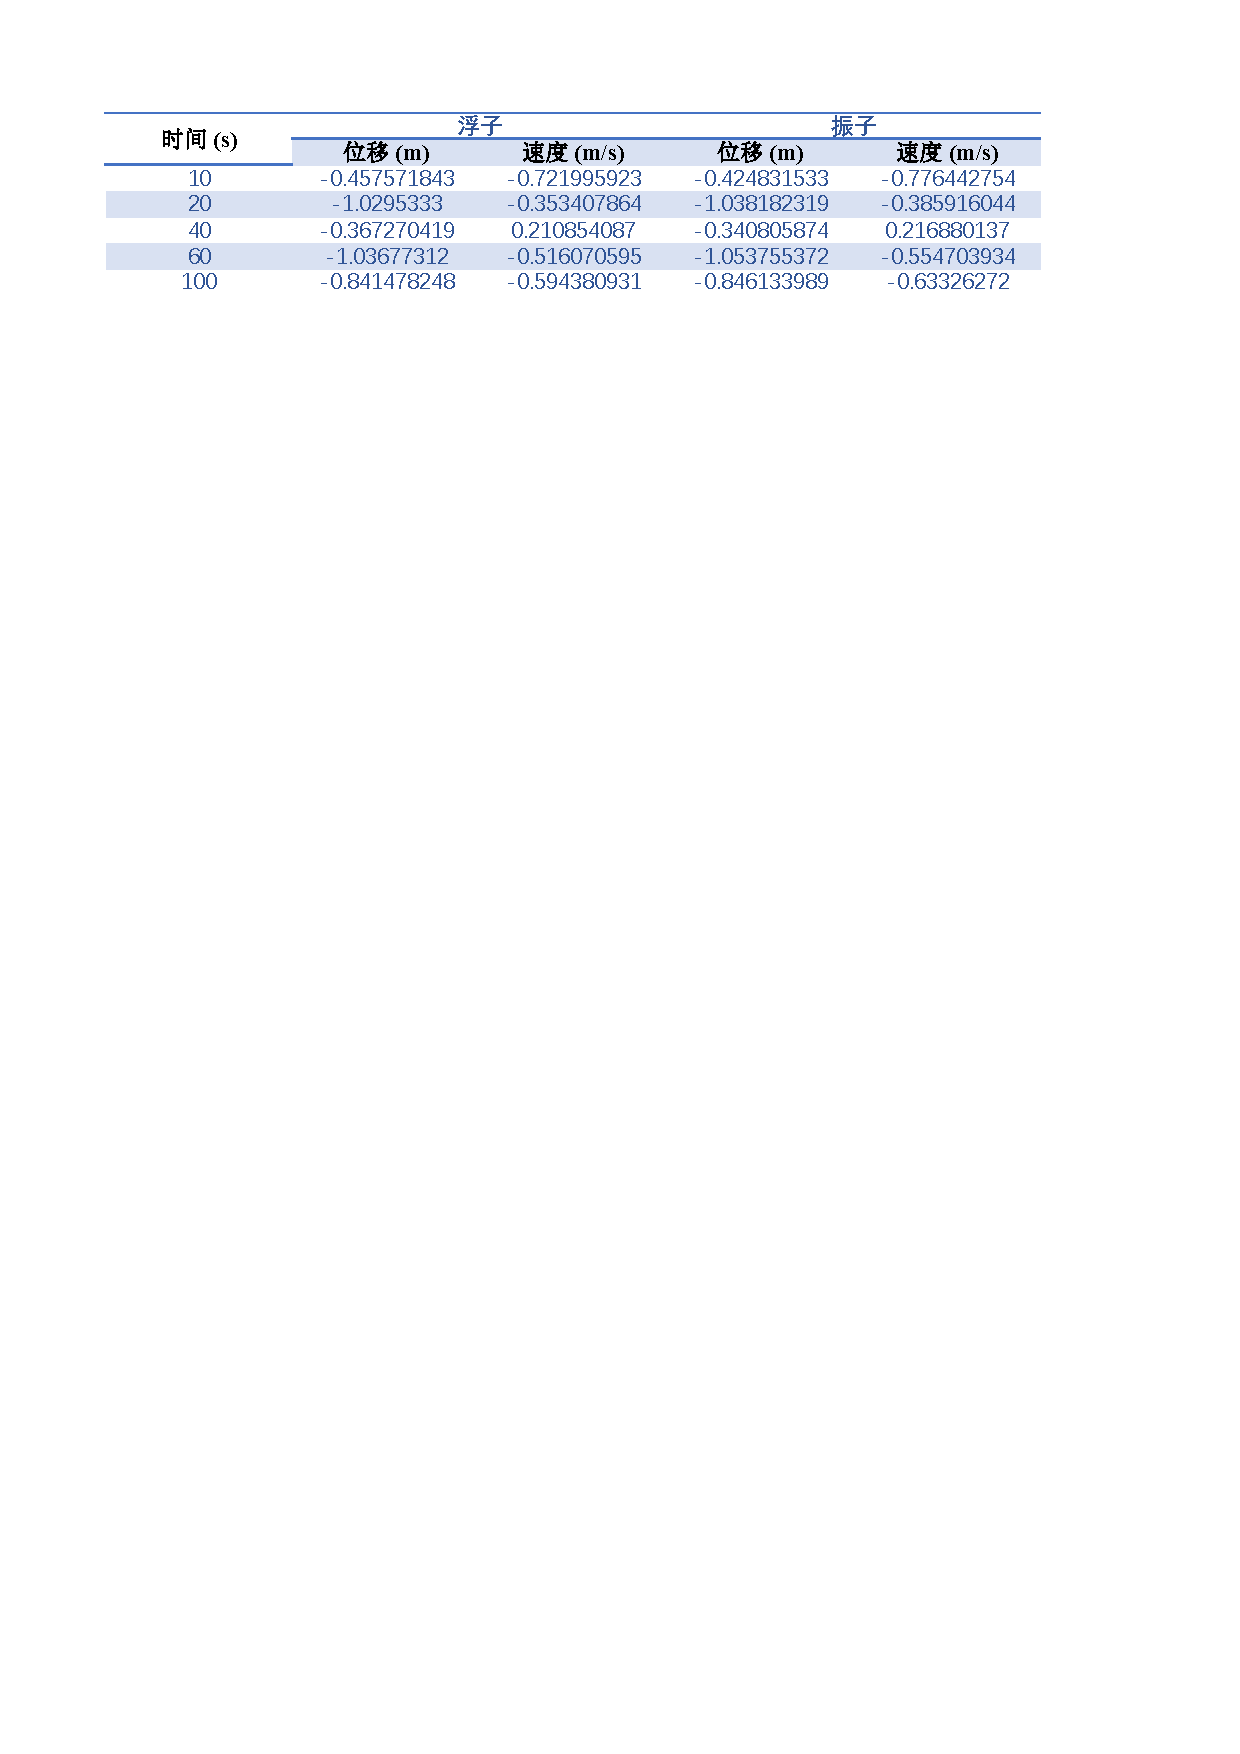
\includegraphics[width=0.7\linewidth]{figures/result1-2.pdf}
	\caption[]{阻尼系数变化时模型计算结果}
	\label{fig:result1-2}
\end{figure}

将计算结果通过matlab绘图函数进行可视化展示,我们得到了如下的震荡曲线。

\begin{figure}[htbp]
	\centering
	\begin{minipage}{0.45\linewidth}
		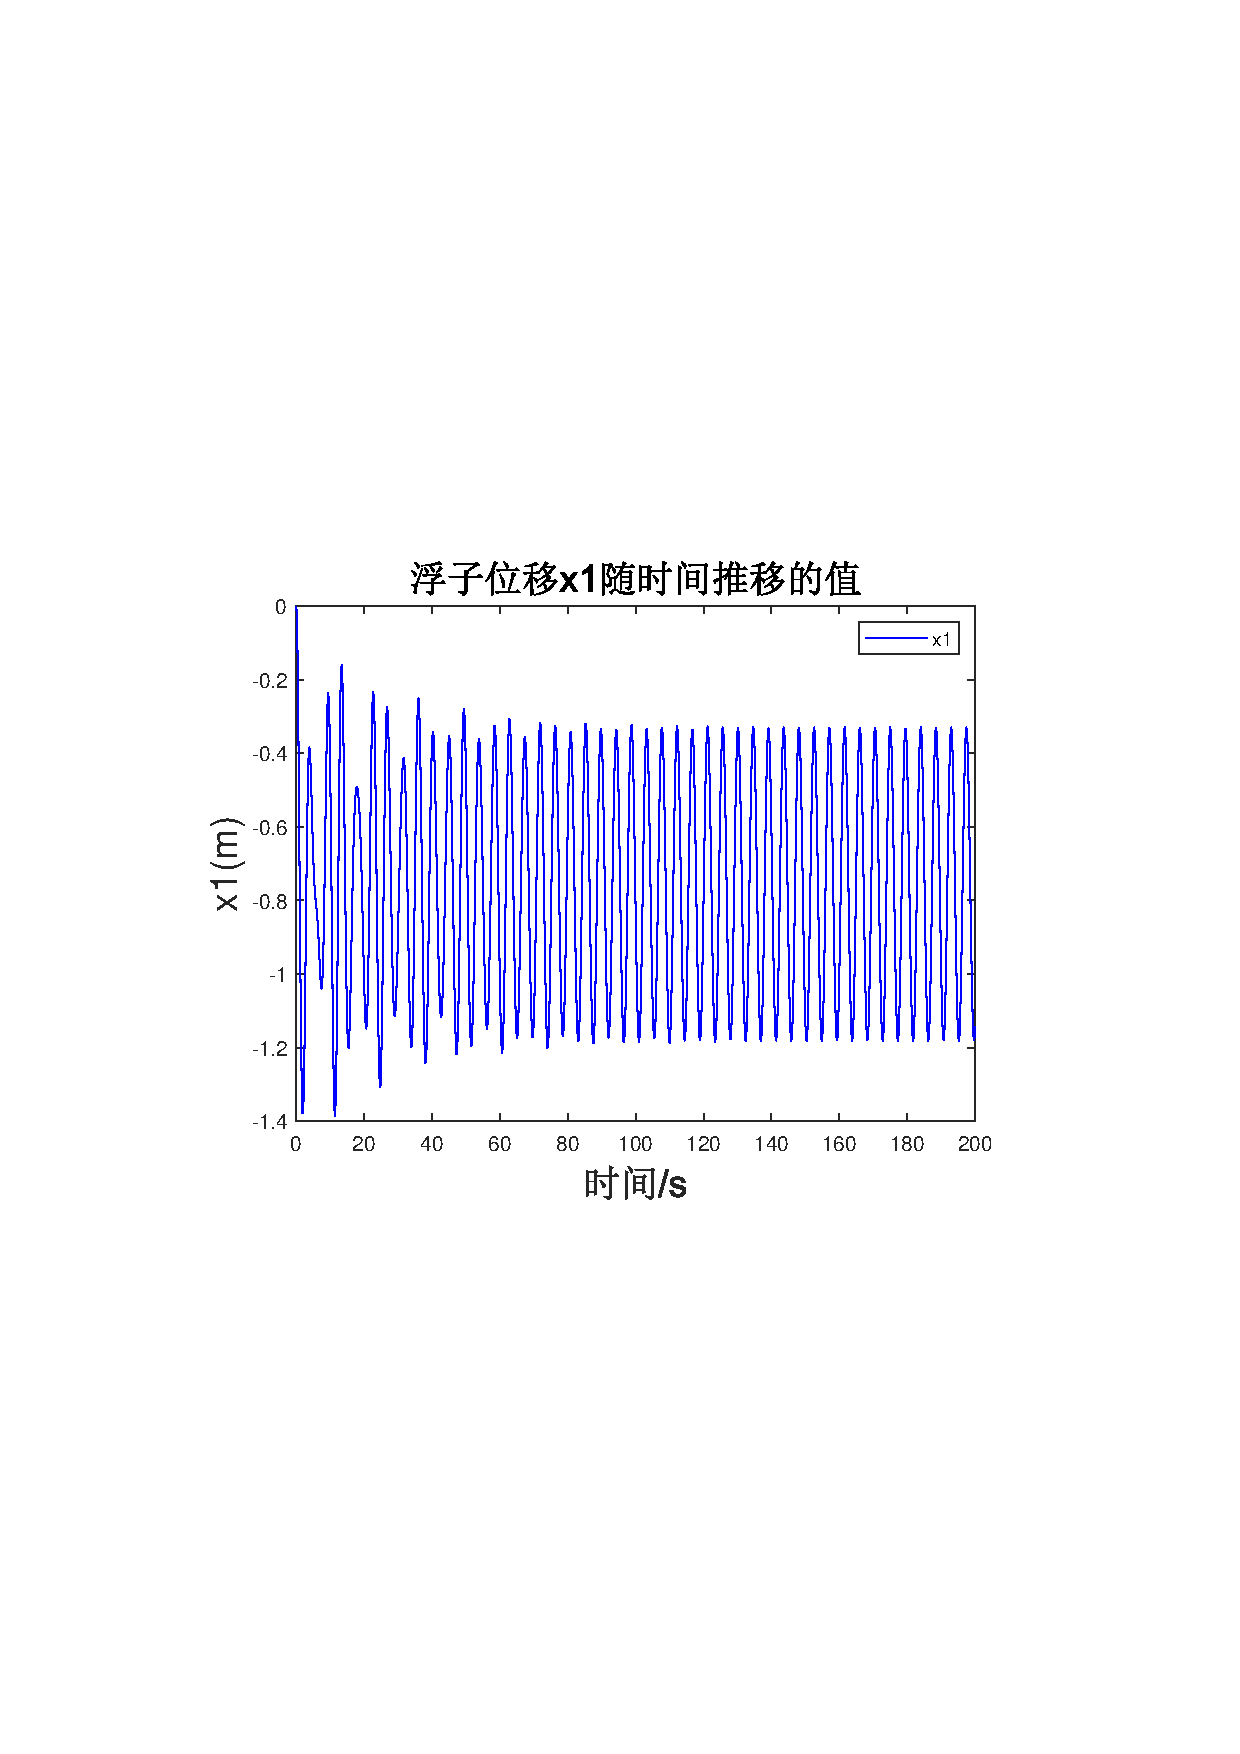
\includegraphics[width=0.9\linewidth]{figures/T1-1浮子位移x1.pdf}
		\label{chutian1}%文中引用该图片代号
	\end{minipage}
	\begin{minipage}{0.45\linewidth}
		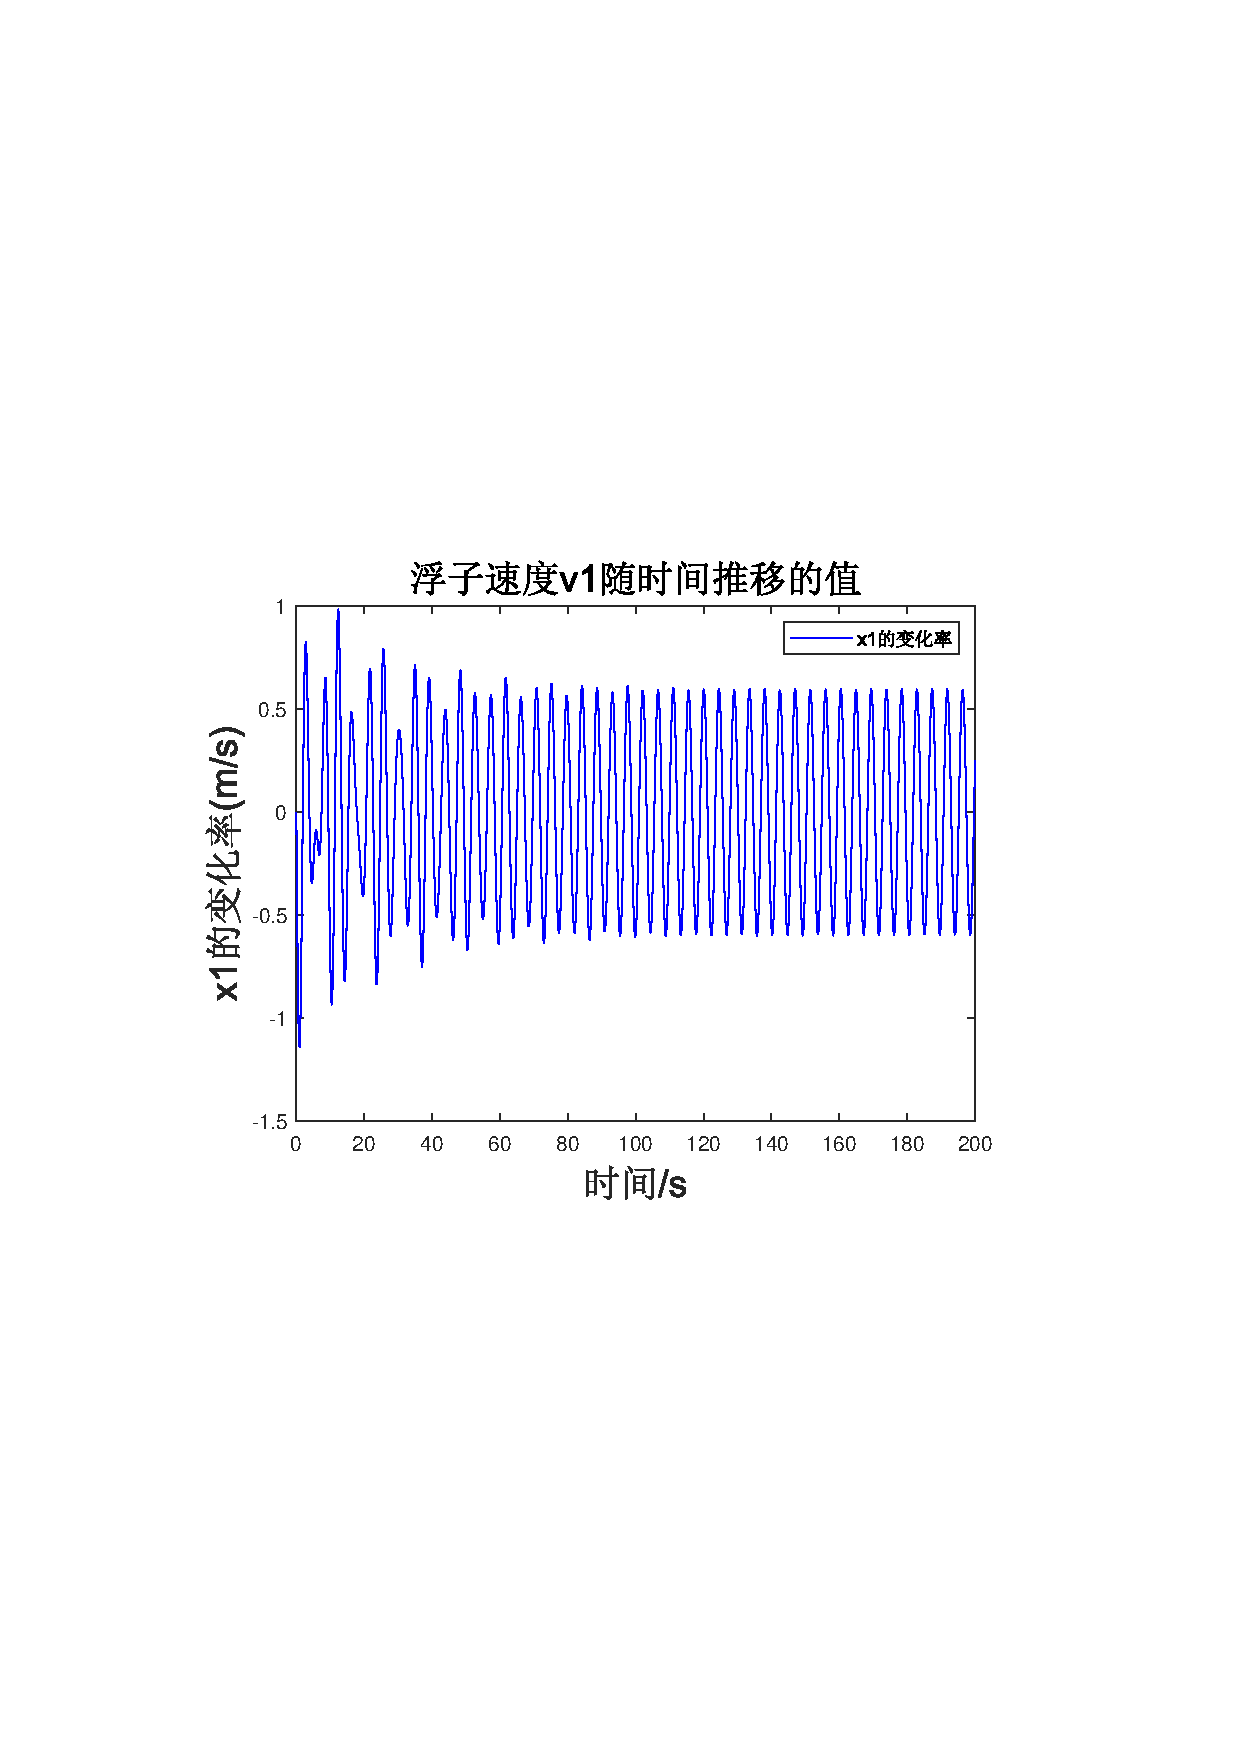
\includegraphics[width=0.9\linewidth]{figures/T1-1浮子速度v1.pdf}
		\label{chutian2}%文中引用该图片代号
	\end{minipage}
	%\qquad
	%让图片换行,
	\begin{minipage}{0.45\linewidth}
		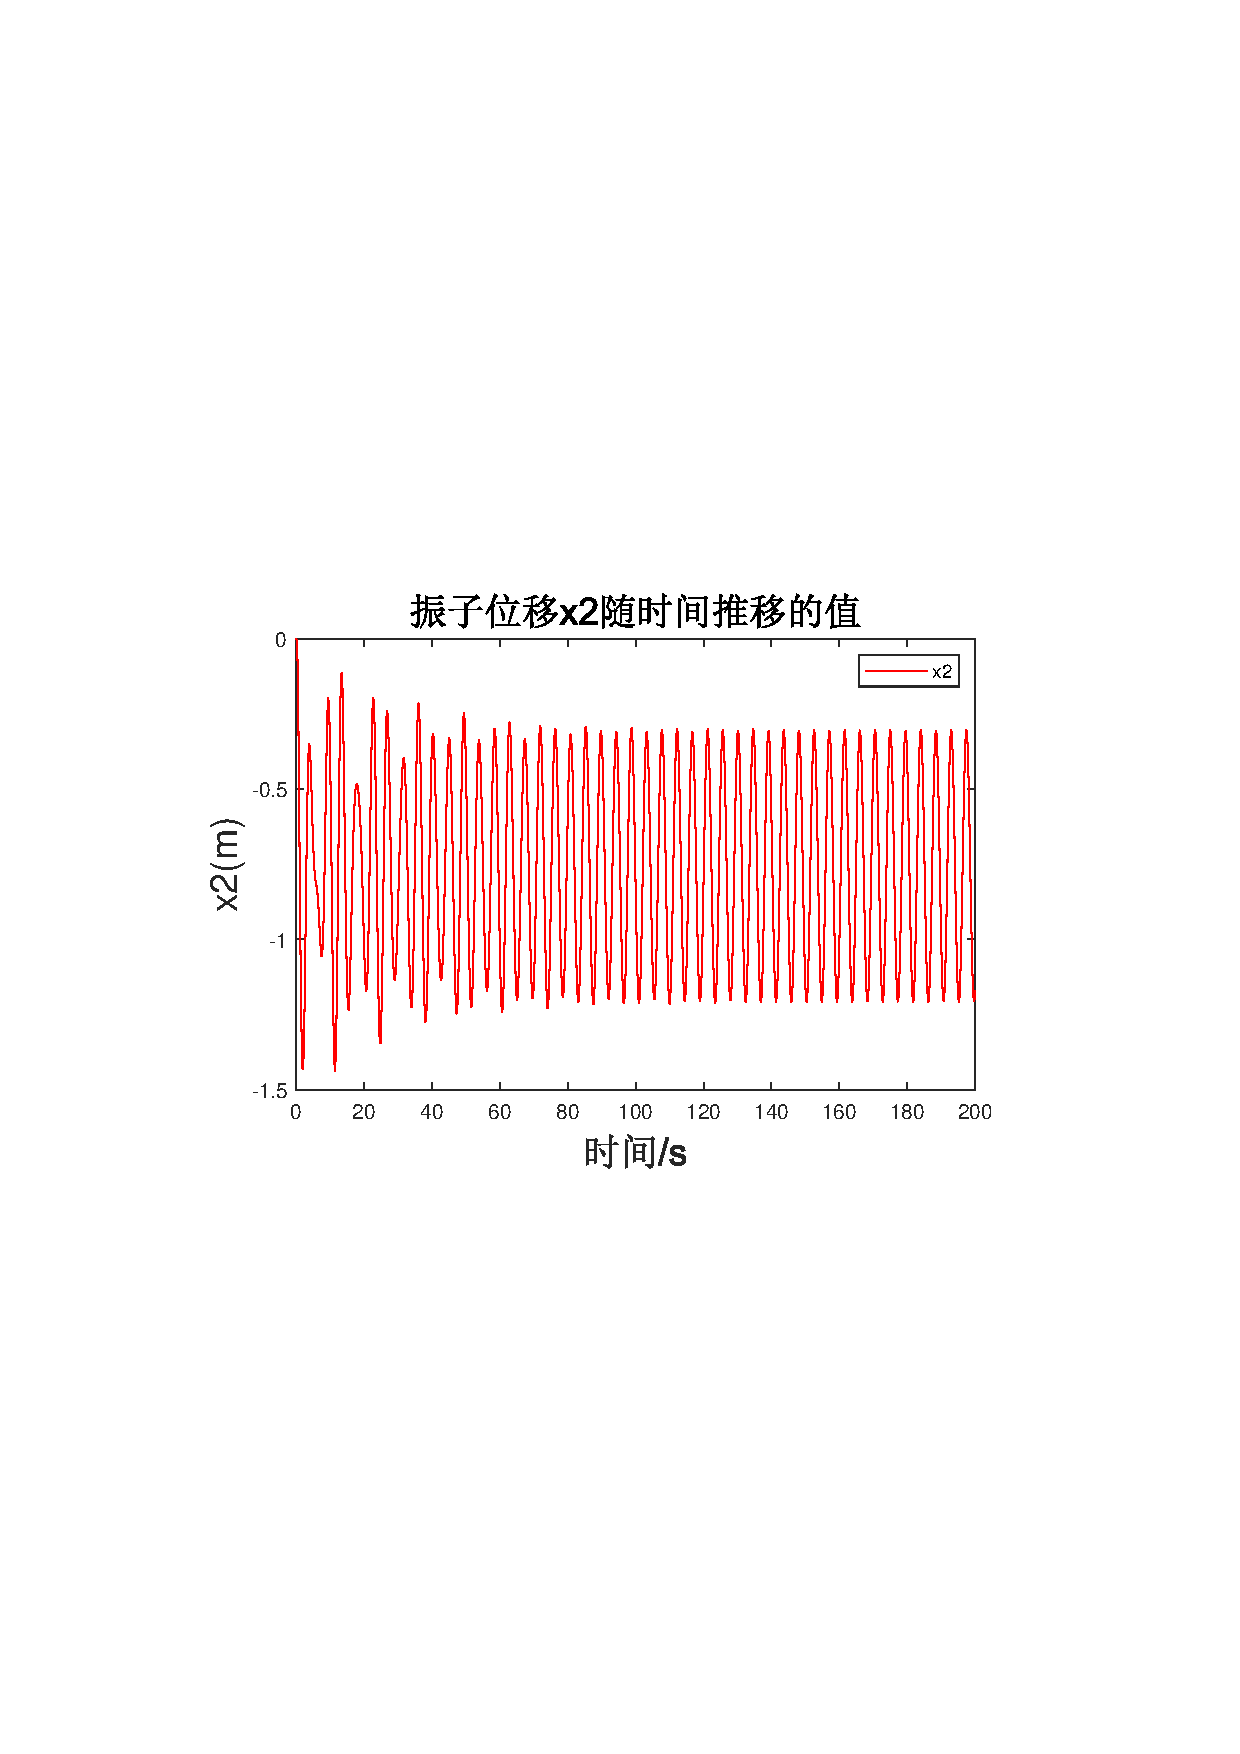
\includegraphics[width=0.9\linewidth]{figures/T1-1振子位移x2.pdf}
		\label{chutian3}%文中引用该图片代号
	\end{minipage}
	\begin{minipage}{0.45\linewidth}
		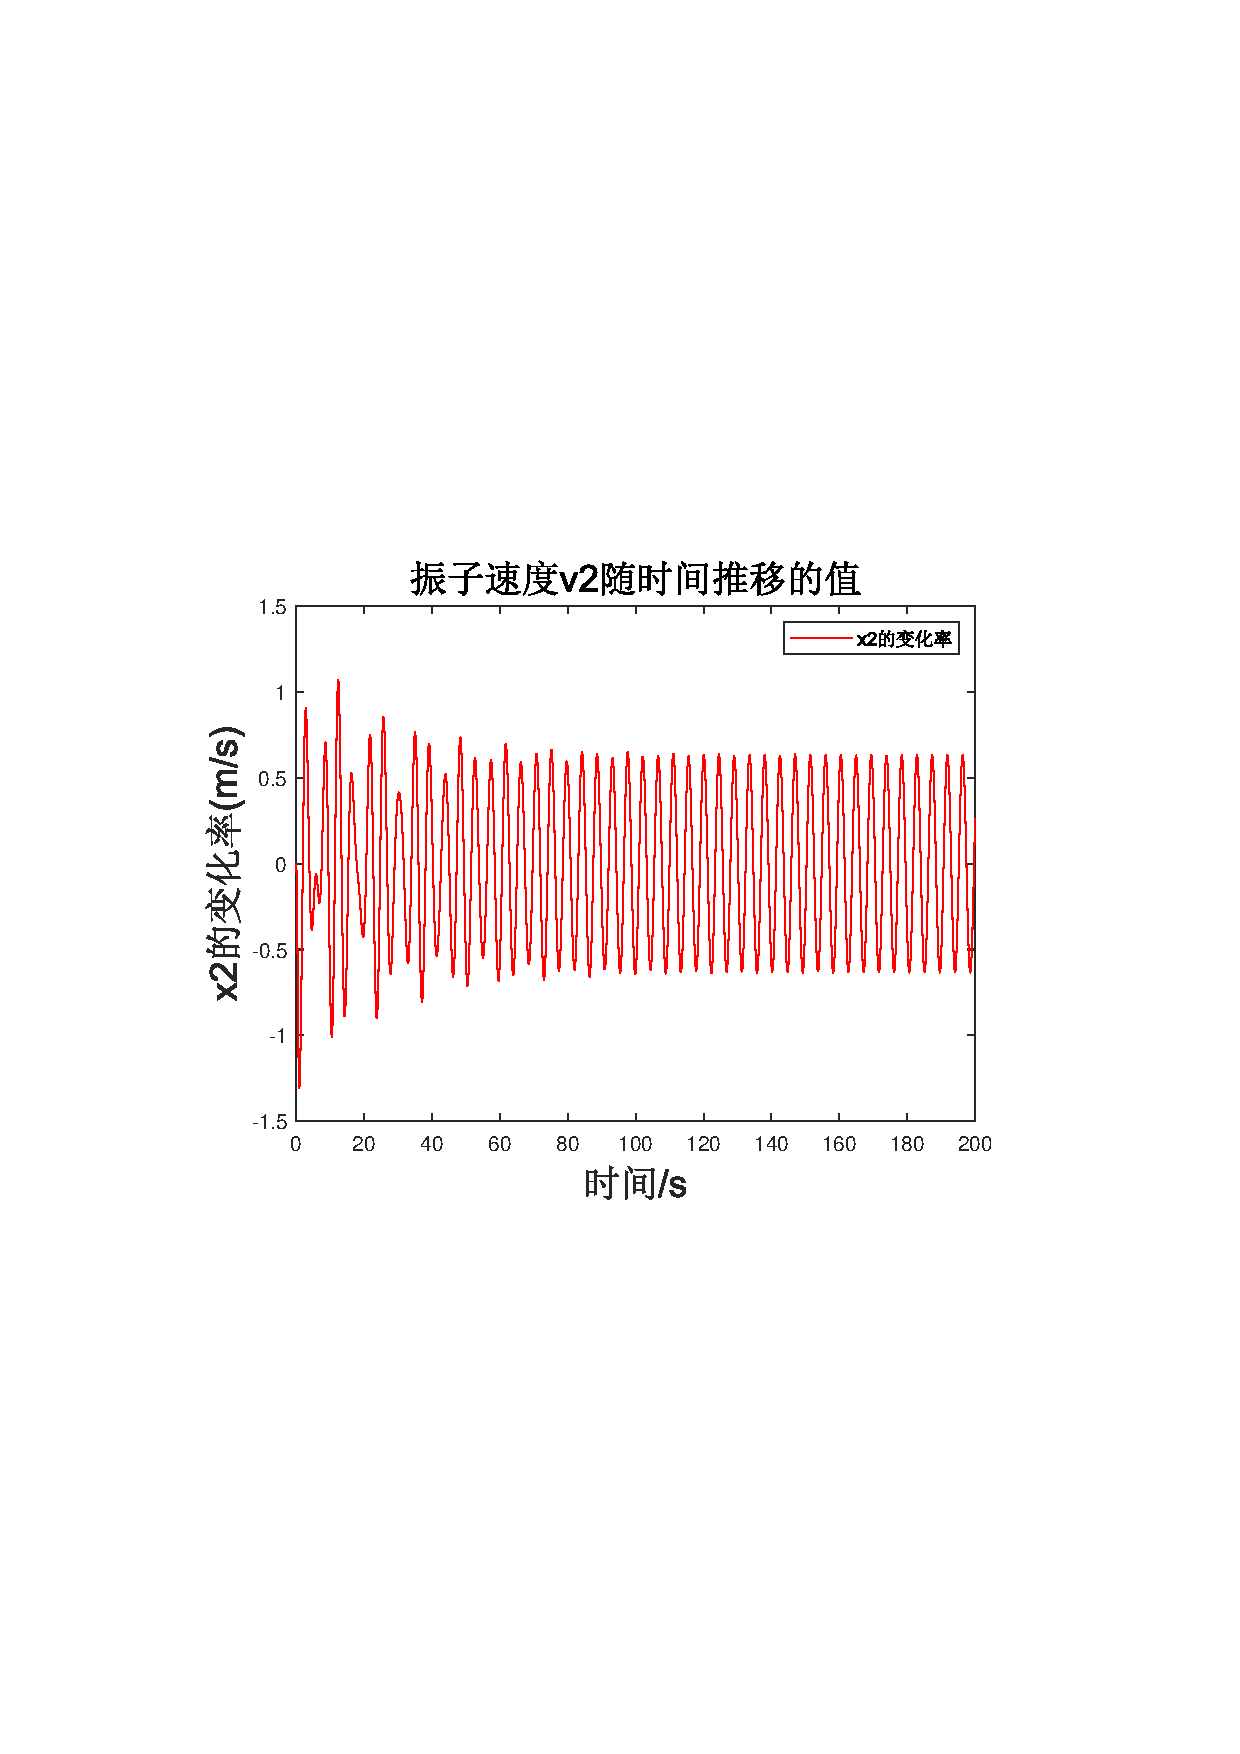
\includegraphics[width=0.9\linewidth]{figures/T1-1振子速度v2.pdf}
		\label{chutian4}%文中引用该图片代号
	\end{minipage}
\caption{阻尼系数恒定时各参数可视化表示}
\end{figure}

\begin{figure}[htbp]
	\centering
	\begin{minipage}{0.45\linewidth}
		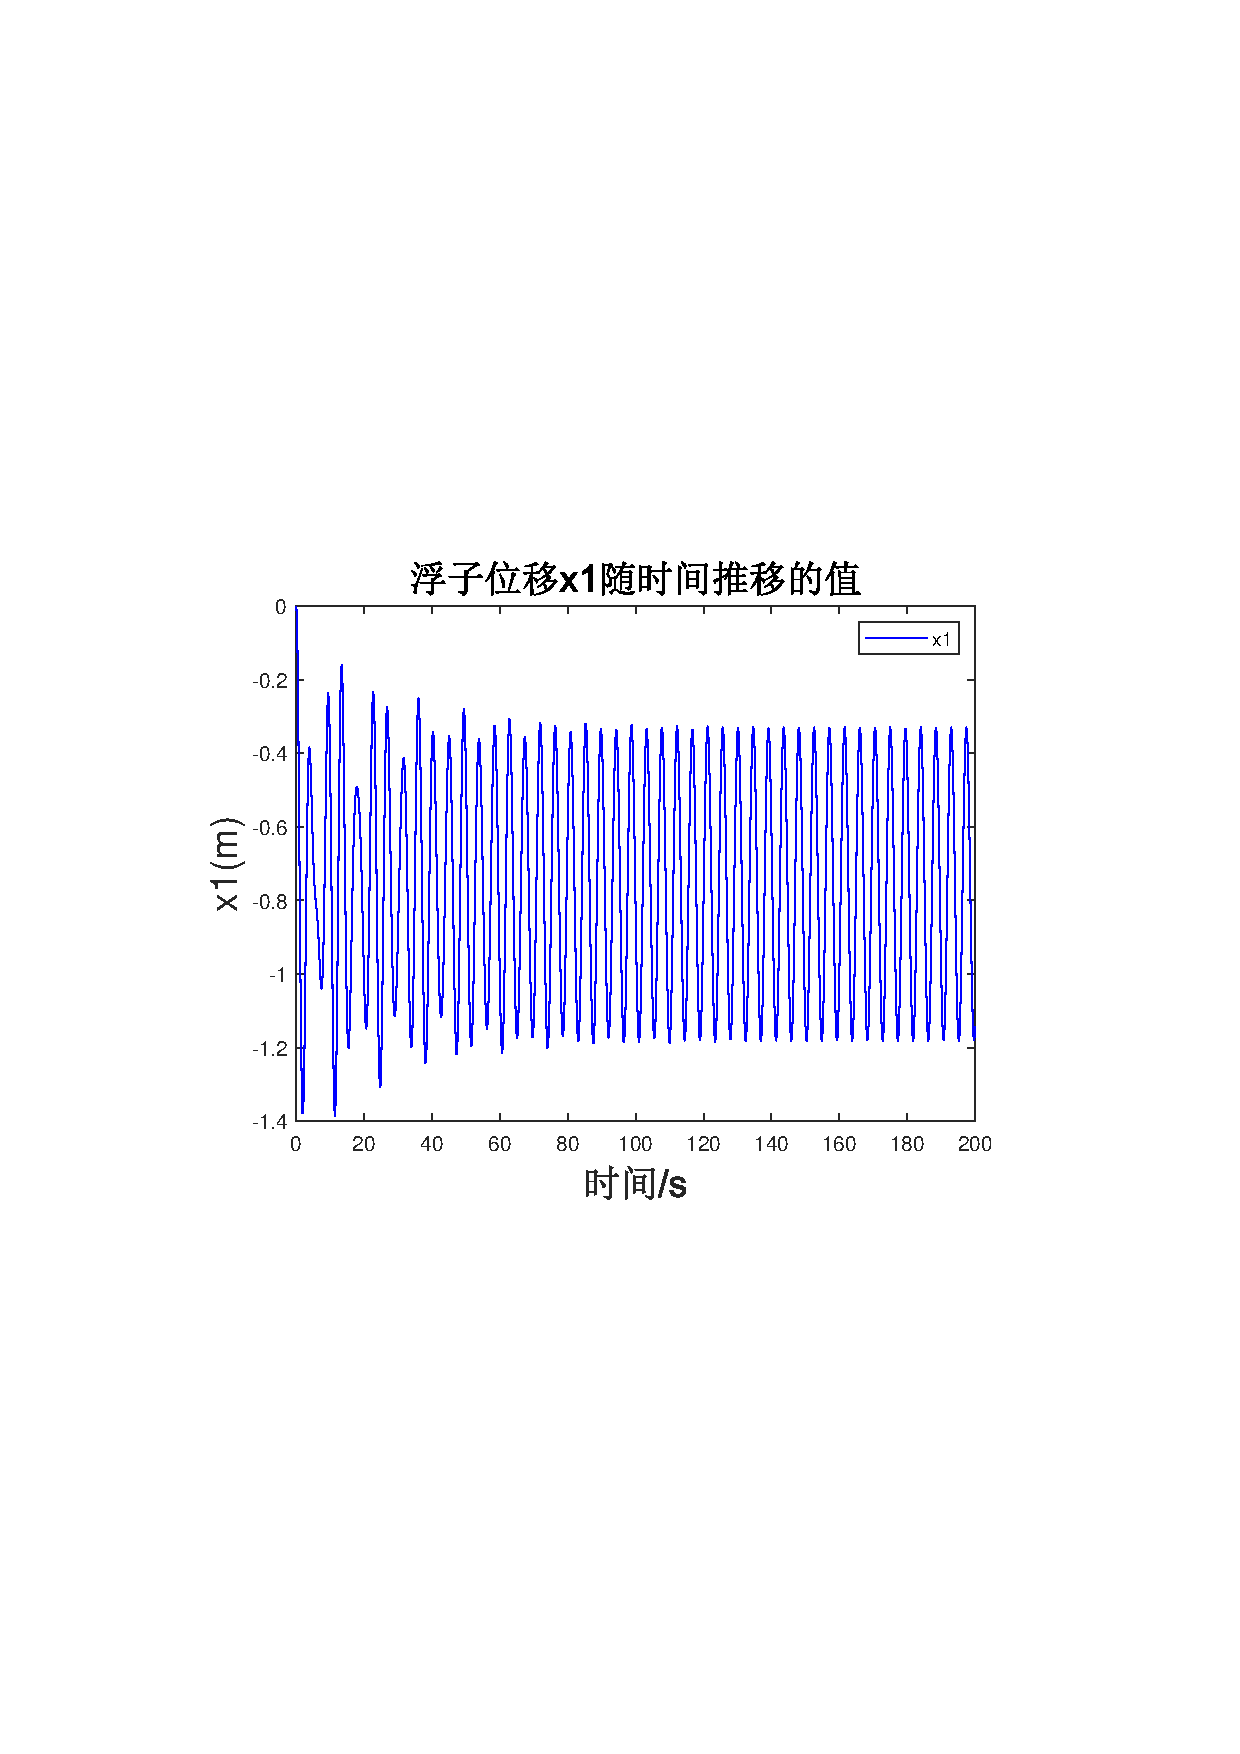
\includegraphics[width=0.9\linewidth]{figures/T1-2浮子位移x1.pdf}
		\label{chutian1}%文中引用该图片代号
	\end{minipage}
	\begin{minipage}{0.45\linewidth}
		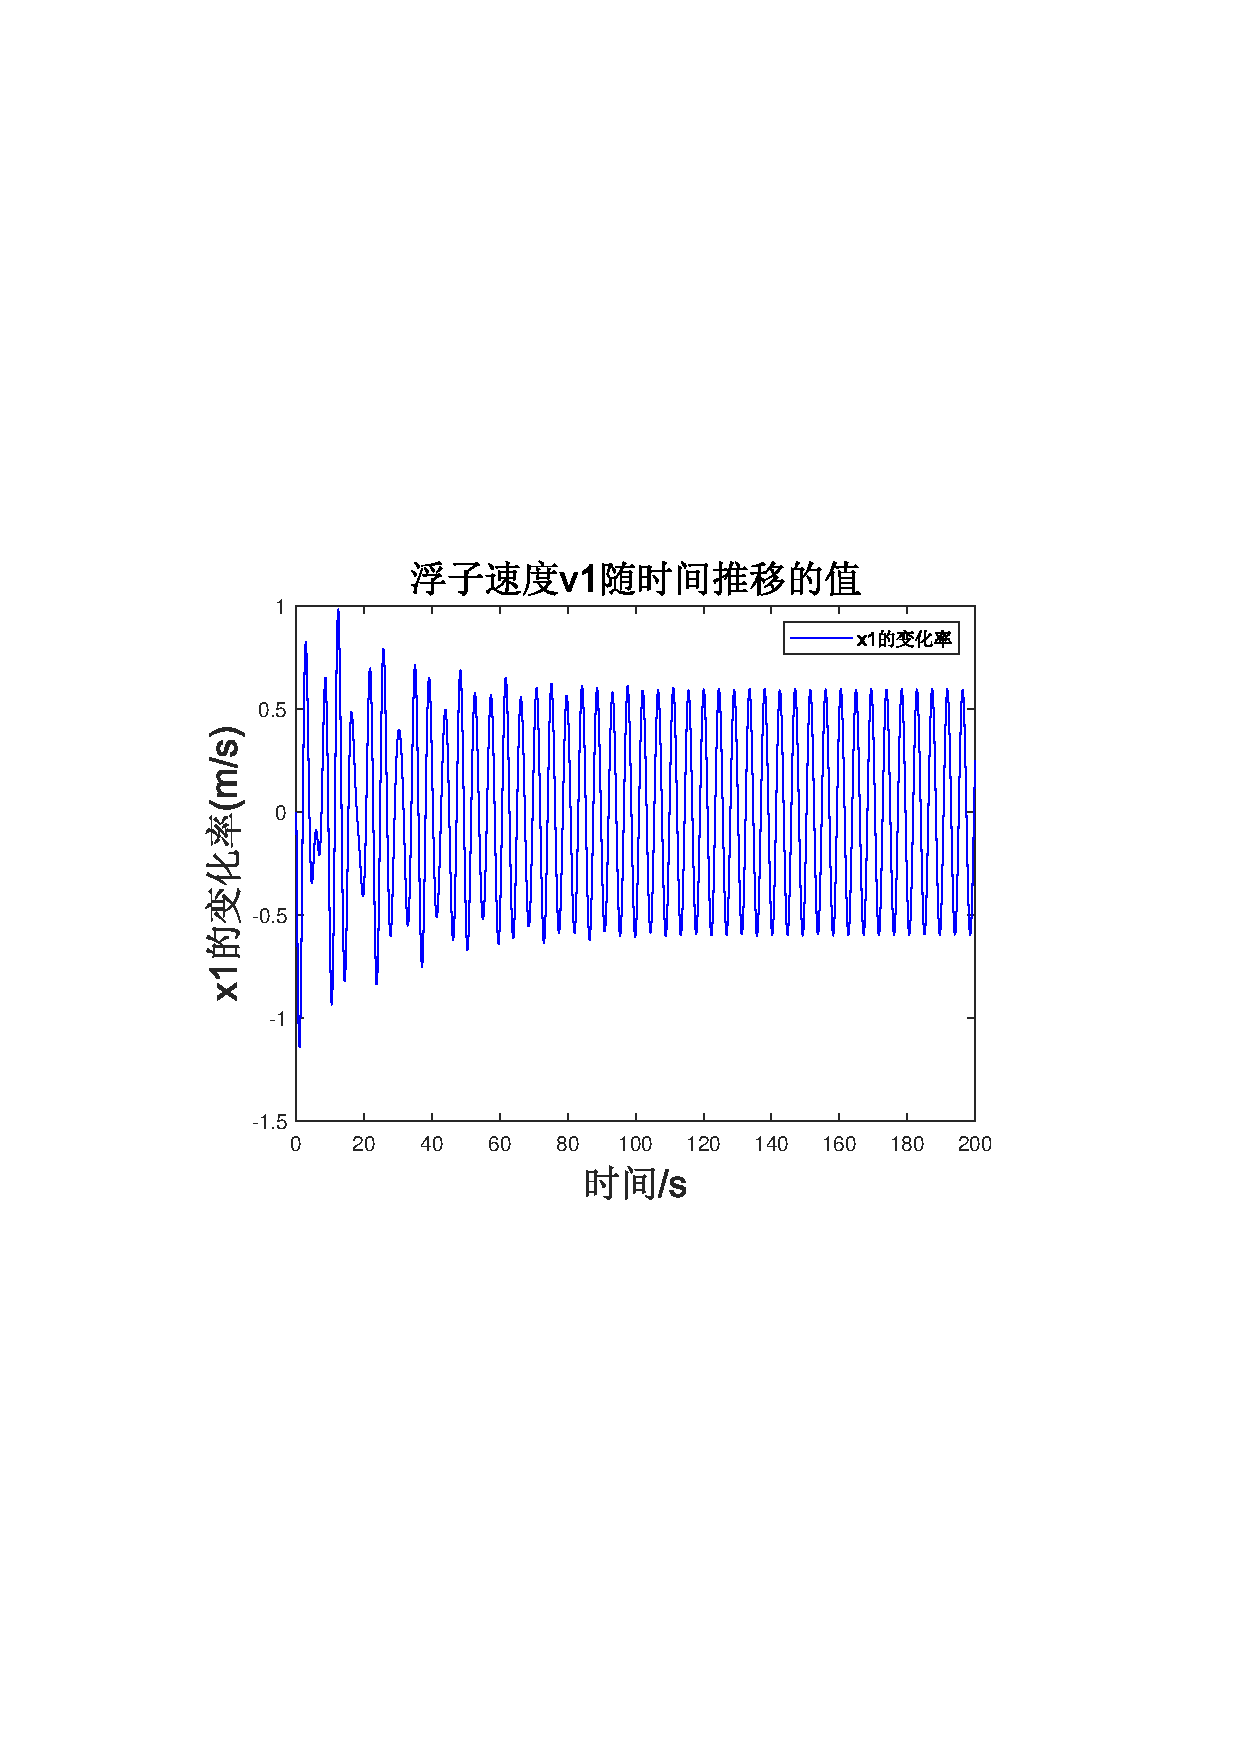
\includegraphics[width=0.9\linewidth]{figures/T1-2浮子速度v1.pdf}
		\label{chutian2}%文中引用该图片代号
	\end{minipage}
	%\qquad
	%让图片换行,
	\begin{minipage}{0.45\linewidth}
		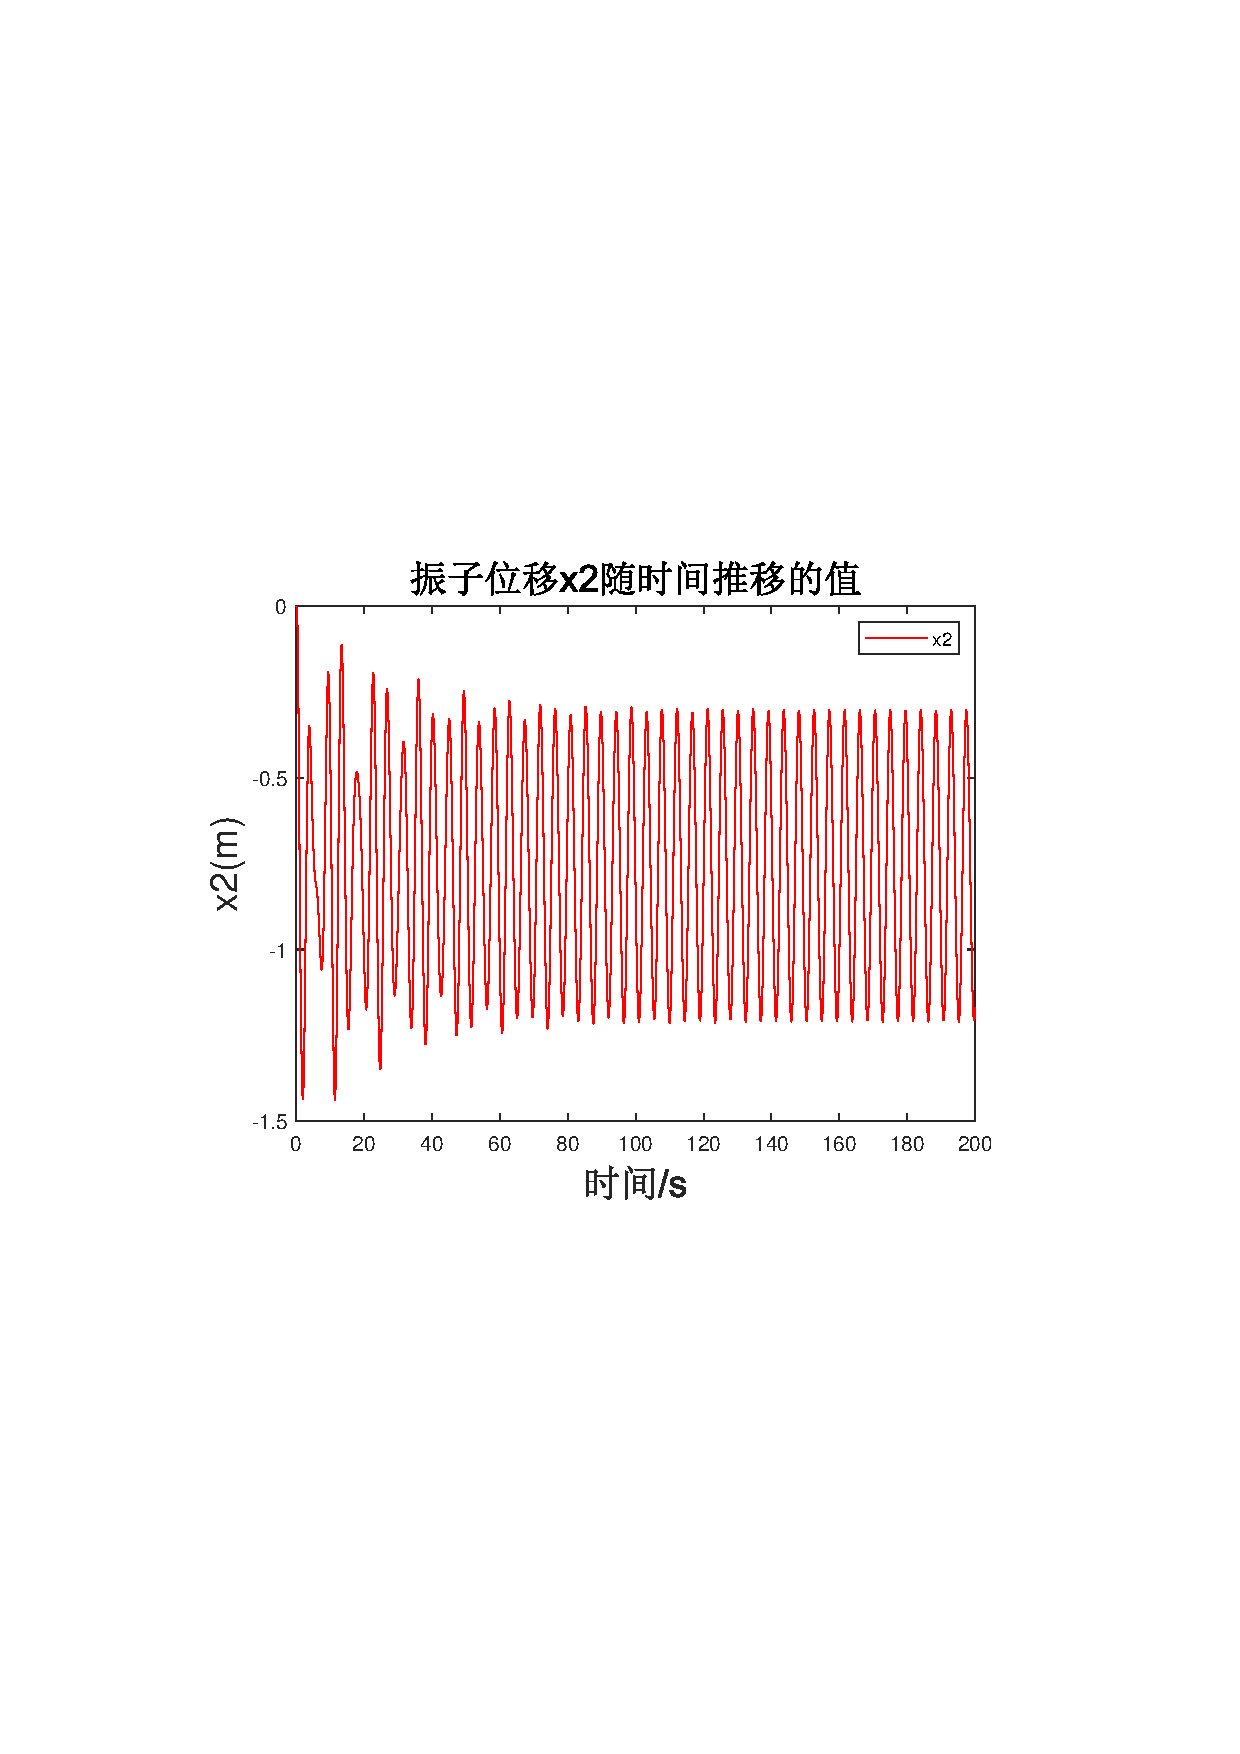
\includegraphics[width=0.9\linewidth]{figures/T1-2振子位移x2.pdf}
		\label{chutian3}%文中引用该图片代号
	\end{minipage}
	\begin{minipage}{0.45\linewidth}
		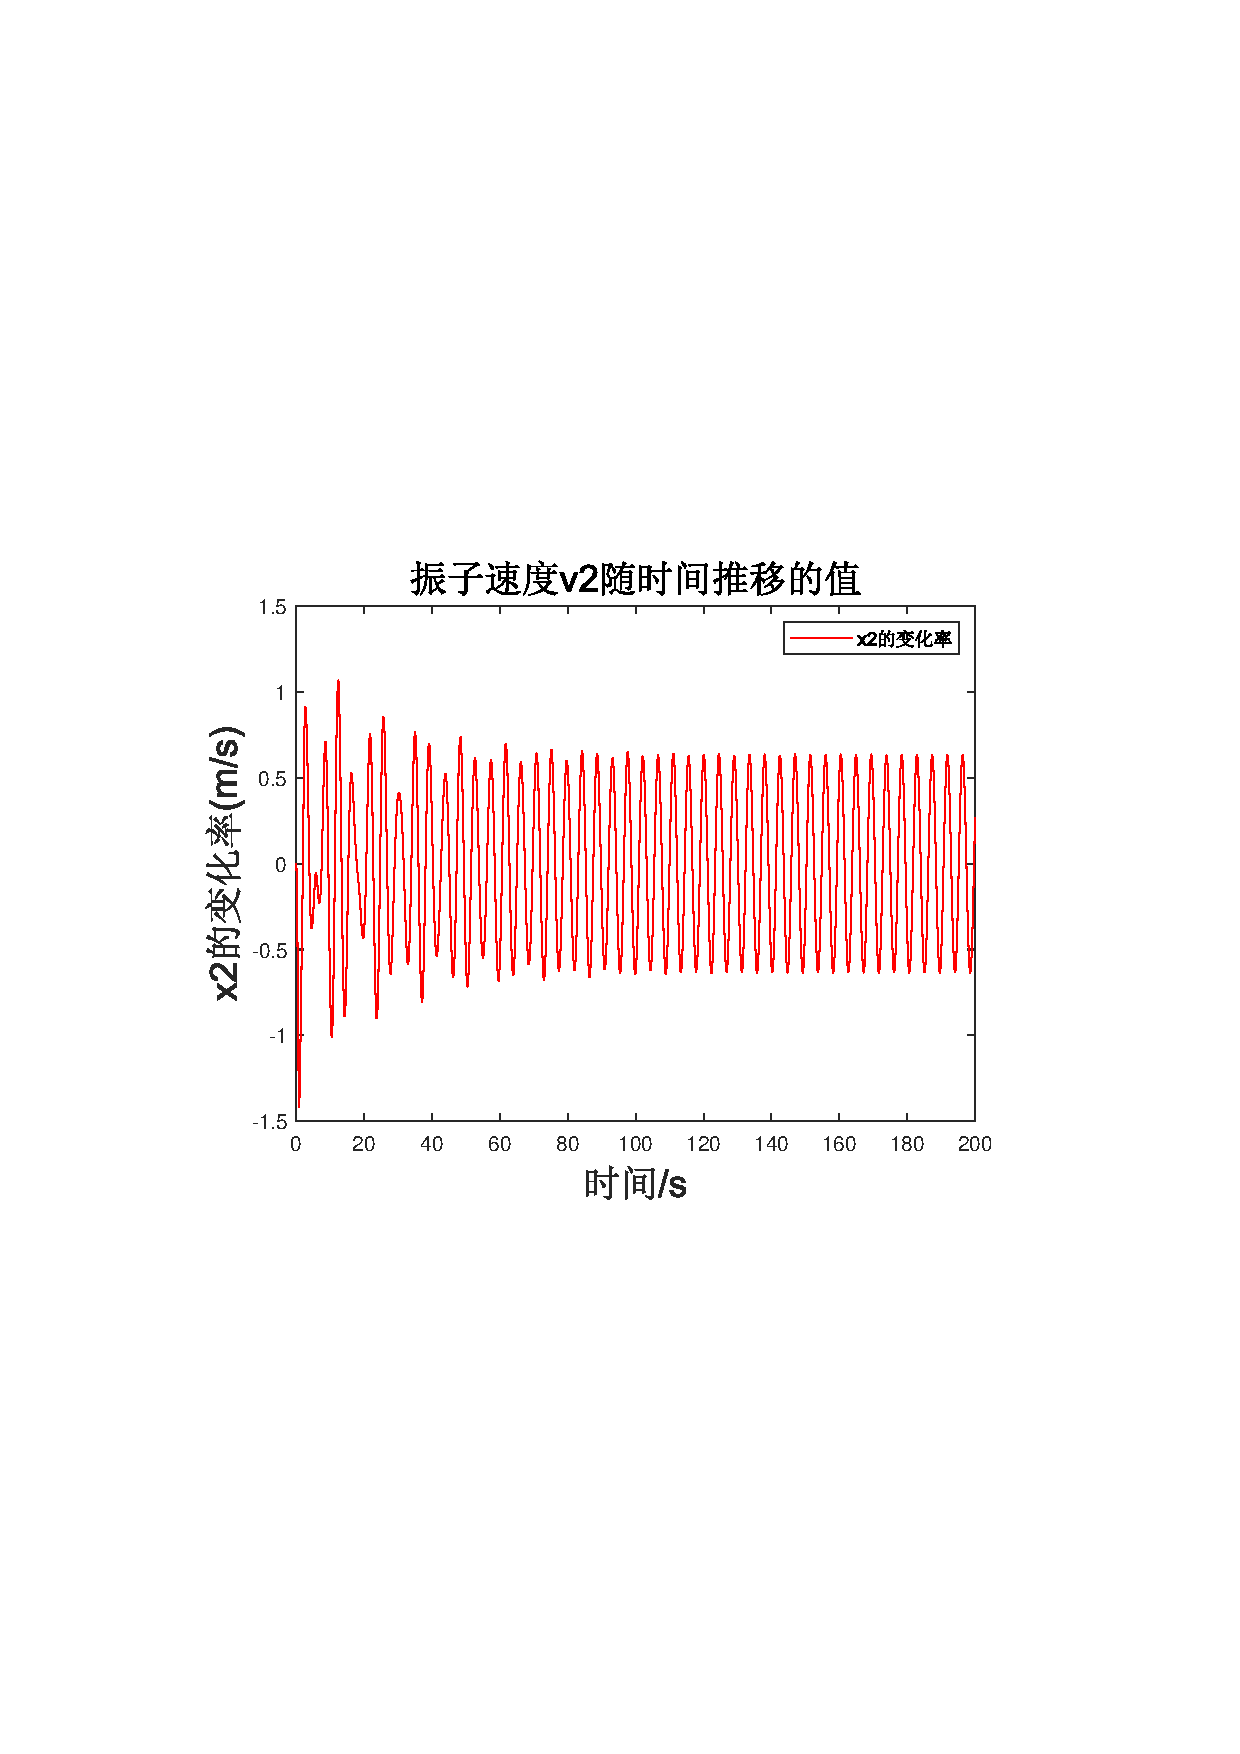
\includegraphics[width=0.9\linewidth]{figures/T1-2振子速度v2.pdf}
		\label{chutian4}%文中引用该图片代号
	\end{minipage}
	\caption{阻尼系数正比与浮子与振子相对速度的1/2次方时各参数可视化表示}
\end{figure}

通过观察图中震荡曲线,我们发现在波浪能装置刚刚开始震荡的时候振幅较大,在运动情况稳定后振幅大小趋同。在每一次震荡中,浮子都会出现完全浸没的情况(x1小于-1m时),势必会对波浪能系统所受到的浮力产生不确定性影响。根据流体力学知识,流体涡流产生的前提是出现速度剪切层。由于浮子快速来回往复运动,浮子与水面之间的相互作用必然会产生速度剪切层。根据本文以及题目中关于无旋环境的假设,我们决定将波浪能装置短时间完全浸没时也可以用公式$f_b(x) = -\rho g\pi R^2x$作为静水恢复力的表达式。

除此之外,我们还可以观察到,浮子与振子的位移在进行震荡运动时的中心位置与静止状态下的平衡位置并不相同。经过重复实验与数据分析,我们认为这一现象的成因在于波浪能装置处于不稳定平衡状态,即浮子与振子在一起进行震荡,造成了复杂的相互作用。我们计算出了浮子与振子的相对速度,如图所示。

\begin{figure}[htbp]
	\centering
	\subfloat[阻尼系数恒定情况]{
		\label{fig:improved1_subfig_a}
		\begin{minipage}[t]{0.5\textwidth}
			\centering
			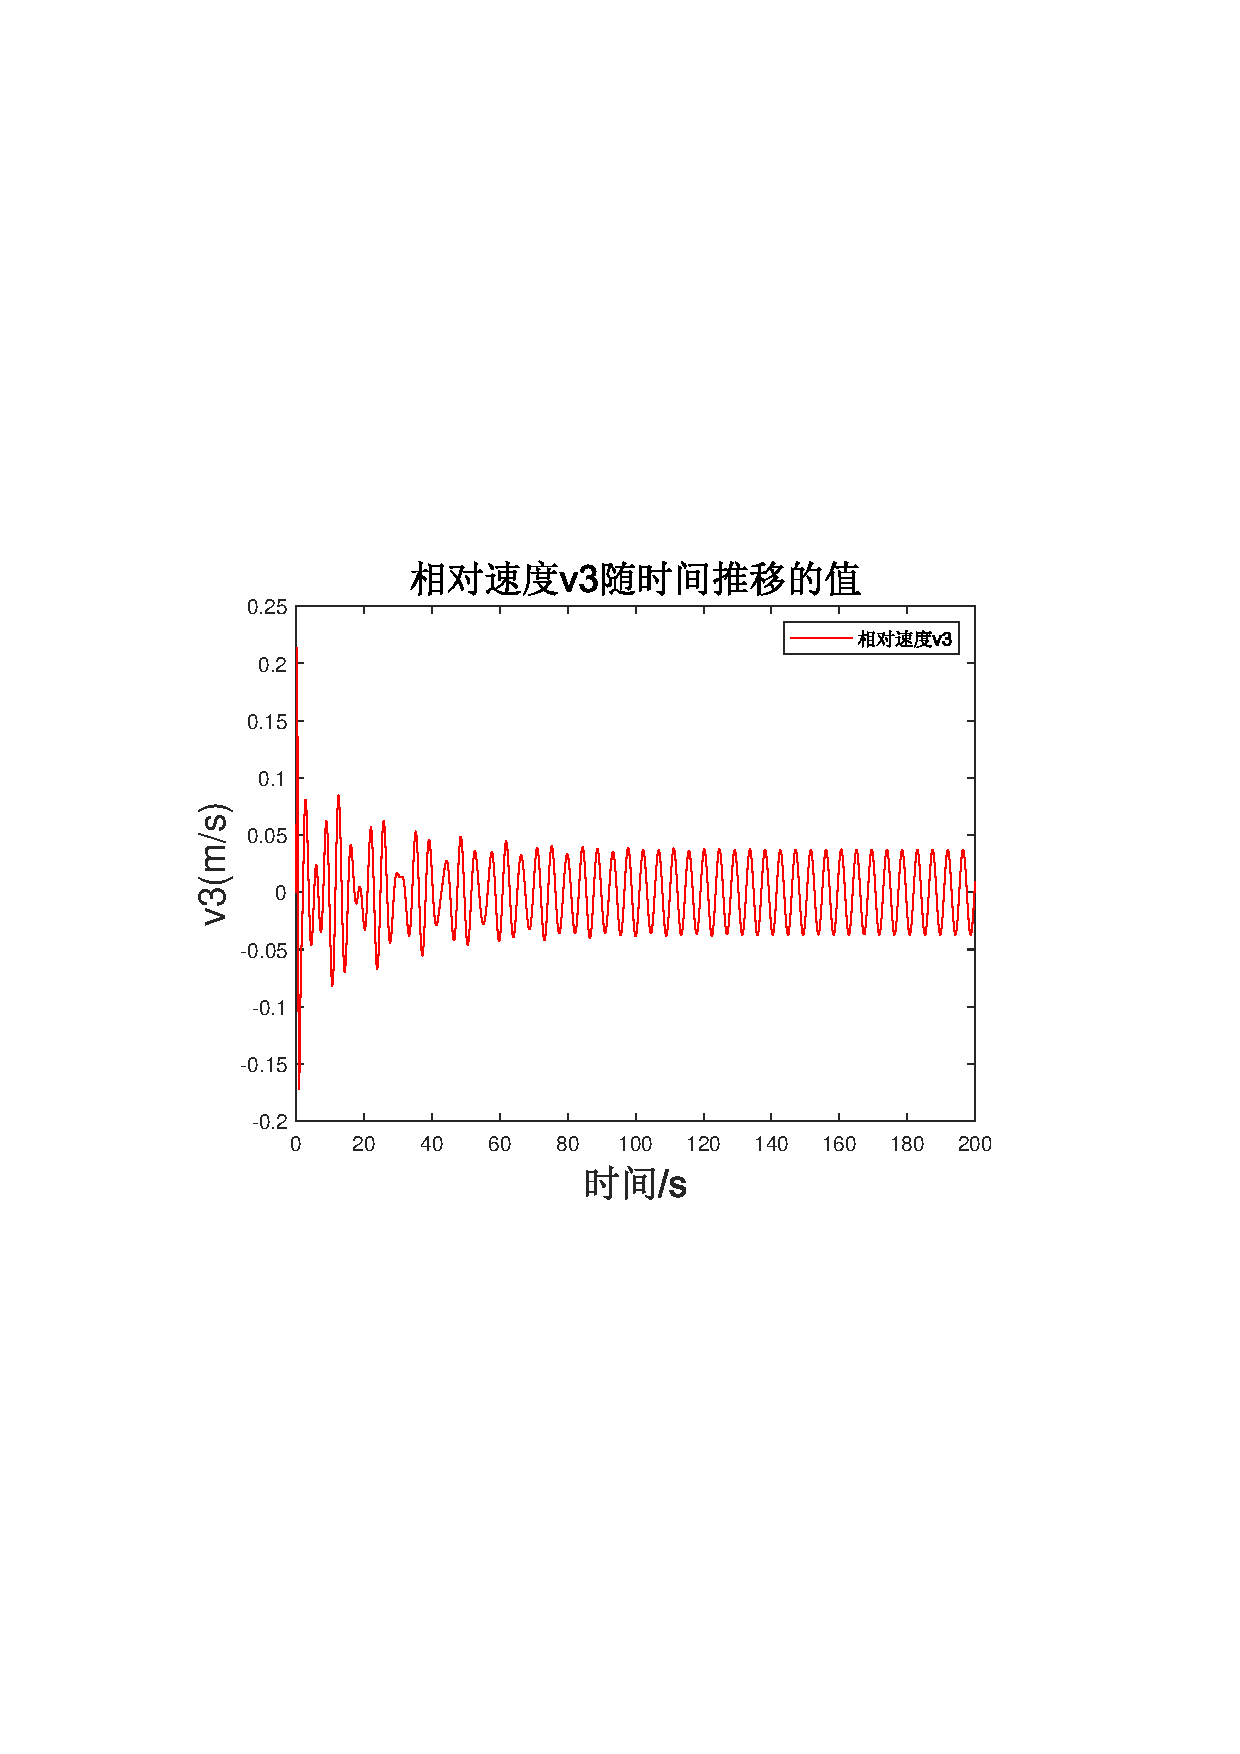
\includegraphics[width=0.8\linewidth]{figures/T1-1相对速度v3.pdf}
		\end{minipage}
	}
	\subfloat[阻尼系数变化情况]{
		\label{fig:improved1_subfig_b}
		\begin{minipage}[t]{0.5\textwidth}
			\centering
			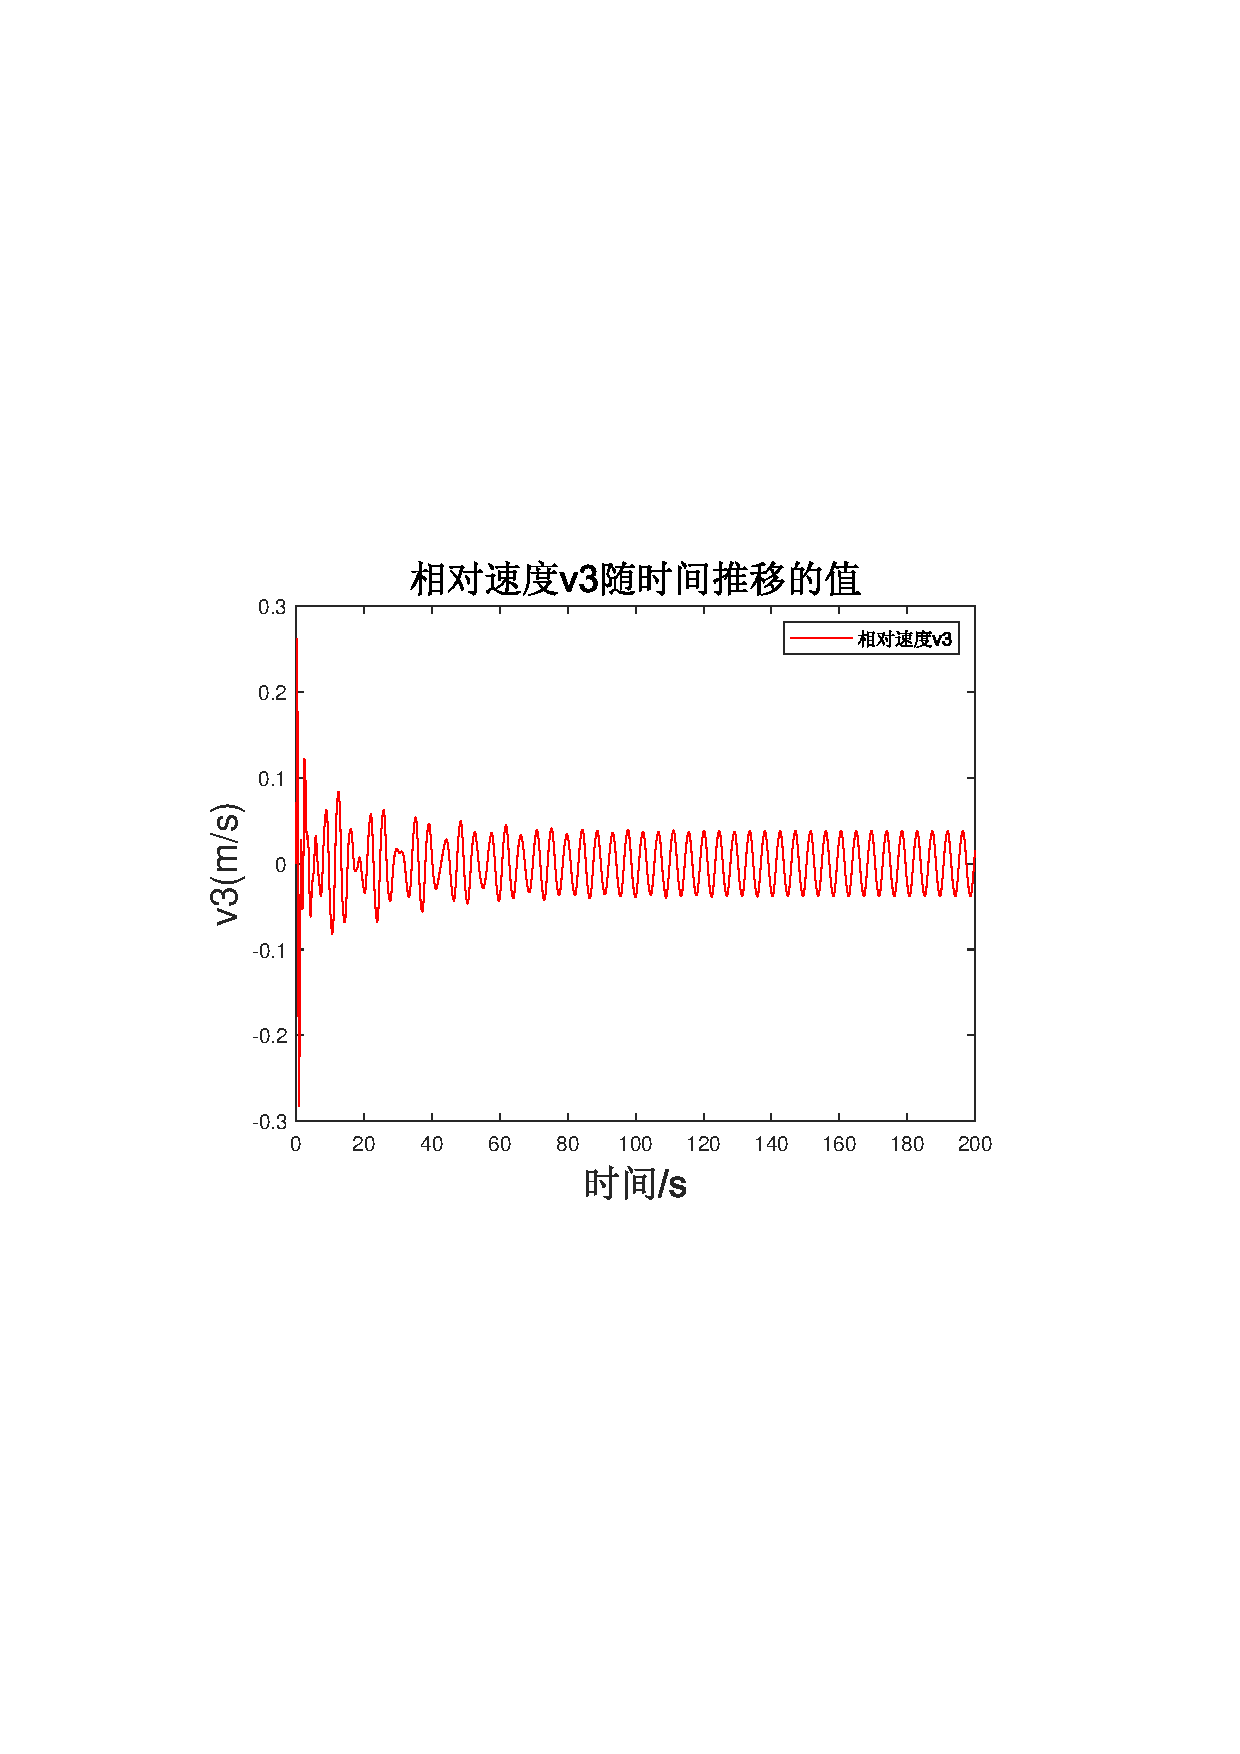
\includegraphics[width=0.8\linewidth]{figures/T1-2相对速度v3.pdf}
		\end{minipage}
	}
	\caption{浮子与振子相对运动速度可视化表示}
\end{figure}



\subsection{问题2模型的建立与求解}

\subsubsection{模型的建立}

问题二仍然针对仅做垂荡运动的波浪能装置展开研究,目的是求解波浪能装置所能获得的最大功率与其对应的最优阻尼系数。由于问题二物理情境与问题一相比无显著差别,故我们基于问题一中的波浪能装置垂荡物理模型求解最优情况下的输出功率与阻尼系数。

根据题目给定条件可知,输出的功率源自波浪能装置中的直线阻尼器。同时,根据假设条件,波浪鞥装置内部各处光滑无摩擦且装置中中轴、底座、各层、PTO质量均可忽略不计。在这种情况下,我们可以假定阻尼器内部无损耗,可以将浮子与振子相对运动对直线阻尼器所做的功全部有效转化。因此,问题等价于求解直线阻尼器阻尼系数与浮子-振子相对运动对阻尼器所做的功的功率之间的对应关系,并求解最优情况下两个变量的值。

当求解阻尼系数恒定情况(问题二第一小问)时,基于动力学知识,我们可以通过如下积分式表示浮子-振子相对运动对阻尼器所做的功:
\begin{equation}
	W_1 = \int f_zdy = \int_{t_0}^{t_1} f_z\dot{y(t)}dt = \int_{t_0}^{t_1}K_z[\dot{y(t)}]^2dt
\end{equation}

式中$f_z=-K_z\dot{y}$为阻尼对振子的作用,$t_0,t_1$分别为积分的起始时间和结束时间。根据第一问的结果,我们知道在波浪能系统起振的时候震荡状态并不稳定,数据并不能代表该装置正常状态的能量输出效果。更好的方式是将$t_0$定为系统进入稳定震荡后的某个时间。

当求解阻尼系数变化情况(问题二第二小问)时,我们需要对积分式的形式进行一定程度的修改:
\begin{equation}
	W_2 = \int f_zdy = \int_{t_0}^{t_1} f_z\dot{y(t)}dt = \int_{t_0}^{t_1}K_z|\dot{y}|^{\alpha} |\dot{y}|\dot{y}dt = \int_{t_0}^{t_1}K_z|\dot{y}|^{\alpha +2} dt
\end{equation}
式中$\alpha$为幂指数(题设条件:阻尼系数与浮子和振子的相对速度的绝对值的幂成正比)。此时阻尼对振子的作用方程变为$f_z=-K_z|\dot{y}|^{\alpha}\dot{y}$。

在求解问题二中的两小问时,我们使用平均功率作为波浪能装置输出功率的代表,其计算公式为:

\begin{equation}
	P_i = \frac{W_i}{t_1-t_0}\quad (i={1,2})
\end{equation}
式中$P_i$为在i情况下波浪能系统的输出功率,i=1表示阻尼系数恒定(求解第一小问),i=2表示阻尼系数变化(求解第二小问)。

\subsubsection{模型的求解}

对于问题二第一小问,问题处于单变量情况。由于遗传算法、二分法没有循环遍历法得出的结果精确,所以我们选定特定步长,采用最基本的循环遍历的方式找到阻尼恒定情况下的所能输出的最大功率表与对应的最优阻尼系数。

首先,我们进行粗略的计算,具体方法是将步长设定为1,对阻尼系数区间 [0,100000]进行全局遍历。遍历结果如图所示。我们在图中标定出了曲线的最大值点,当阻尼系数取31121时输出功率取得最大值298.2544W。


对于粗略计算所得结果附近的区域,我们换用更小的步长0.01,对阻尼系数区间[31000,32000] 进行遍历。遍历结果如图所示。我们在图中标定了曲线的最大值点,当阻尼系数取31120.10时输出功率取得最大值298.2580W。我们可以观察到图中出现了较为显著的波动情况,这是由于输出功率是根据浮子-振子相对运动速度求得,且该相对运动速度本身具有较强的波动性。



\begin{figure}[h]
	\centering
	\subfloat[阻尼系数恒定-粗略计算]{
		\begin{minipage}[t]{0.49\textwidth}
			\centering
			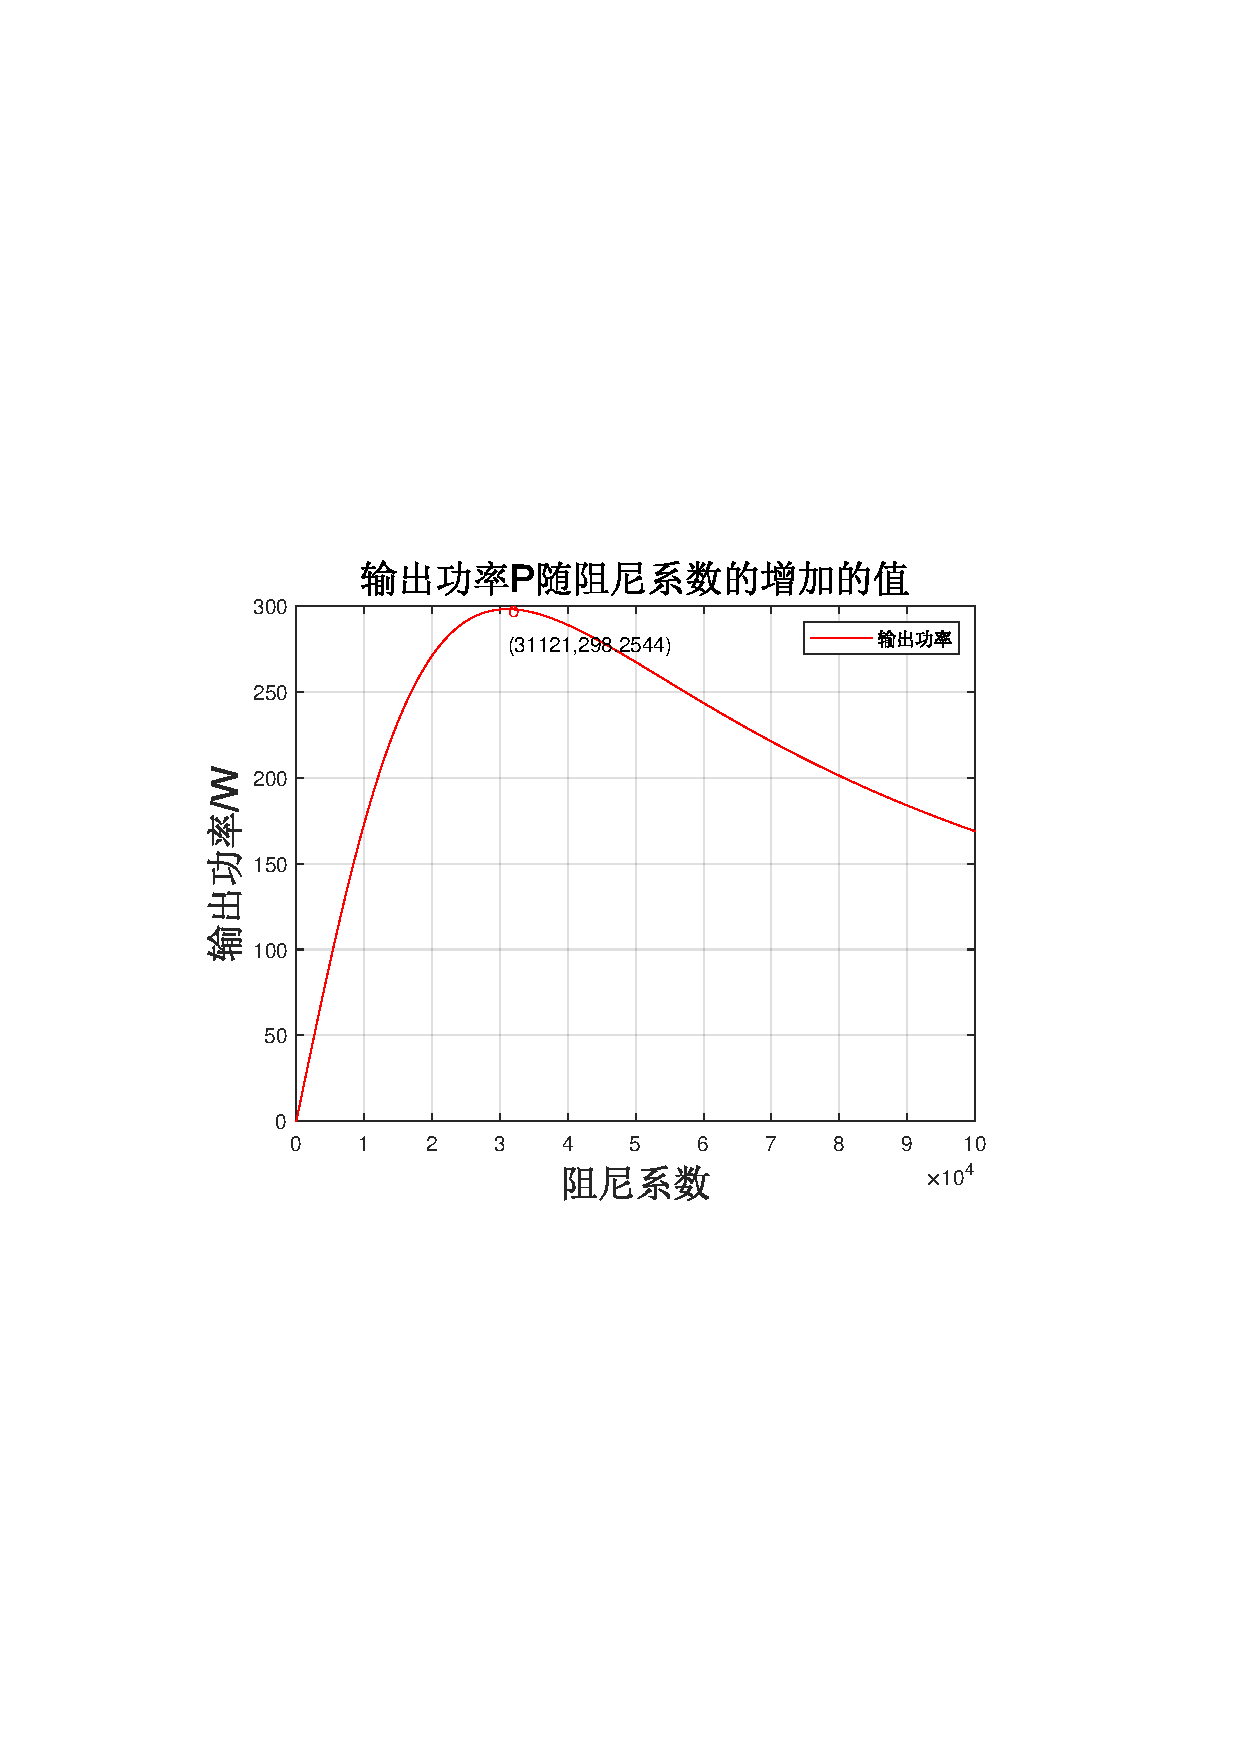
\includegraphics[width=0.8\linewidth]{figures/T2-1遍历步长为1.pdf}
		\end{minipage}
	}
	\subfloat[阻尼系数恒定-精细计算]{
		\begin{minipage}[t]{0.49\textwidth}
			\centering
			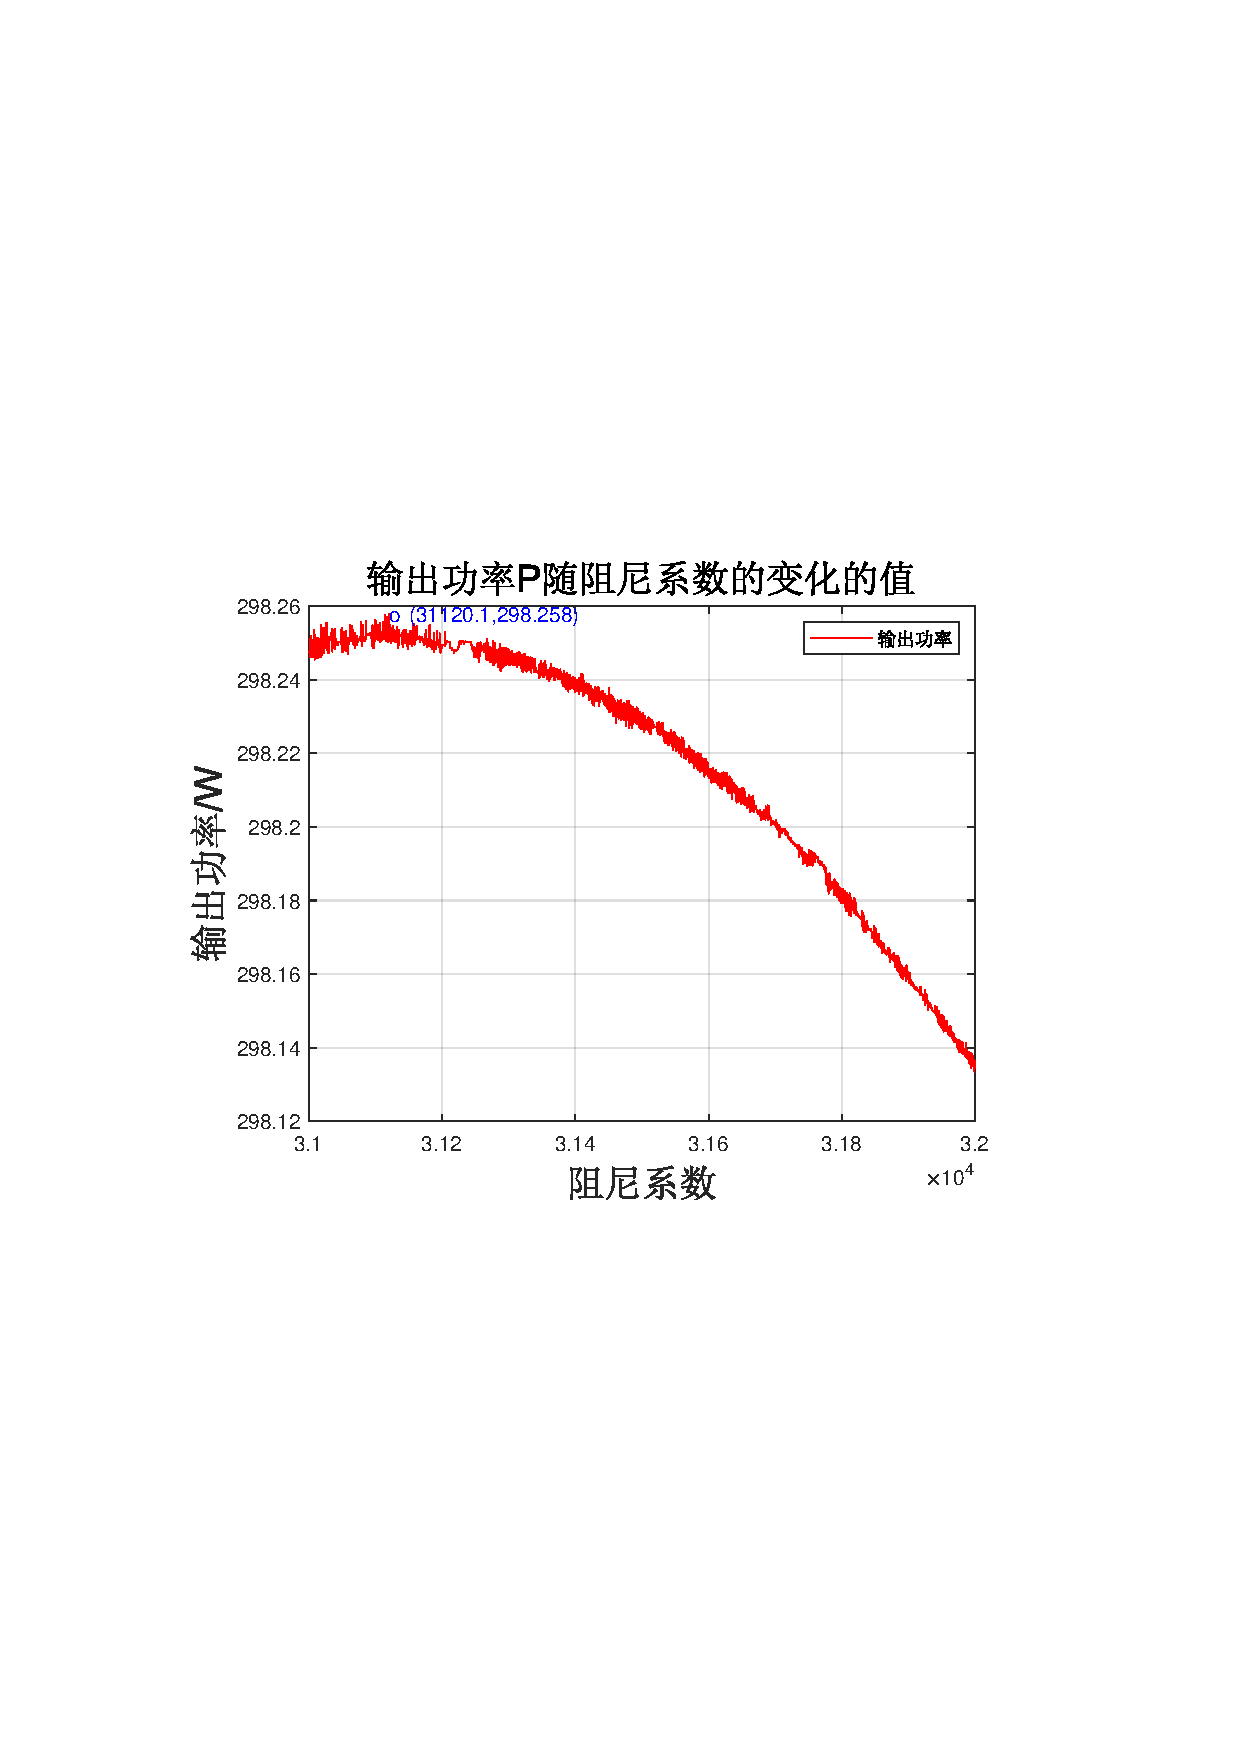
\includegraphics[width=0.8\linewidth]{figures/T2-1遍历步长为0.01.pdf}
		\end{minipage}
	}
	\caption{遍历法求解问题二第一小问的结果}
\end{figure}


除了遍历法外,我们还尝试使用二分法解决问题二第一小问,结果如图所示。可以发现使用不同算法所得出的结果几乎完全相同。但是经过我们多次重复测试,发现二分法在解决单变量优化问题时非常容易陷入局部最优解。这个现象产生的原因是所研究的目标曲线并非严格凸函数,而是包含了一定程度的震荡。


对于问题二第二小问,由于阻尼系数不再固定,问题变得更加复杂,使用遍历法会面临高昂的时间与空间复杂度,令人无法承受。因此,我们使用了遗传算法求解阻尼系数变化时的最大输出功率与相对应的阻尼系数。遗传算法的主要原理是模仿生物界自然选择的方式,通过“选择”、“变异”、“交叉”的方式积累数据优化的“性状”,最后求解优化问题。该算法的优点是相比传统优化算法运行更加迅速的向优化目标收敛,缺点是该算法存在一定的随机性,存在一定的陷入局部最优解的风险。

在有关波浪能装置输出功率的求解中“选择”函数为优化目标函数,即装置输出功率;“变异”与“交叉”函数包括两个重要参数:突变概率pm与交叉概率pc,通常pc处于0.6左右,保证通过交叉及时保存变异出来的被“选择”函数选择的解;pm处于0.001左右,pm过高会导致被“选择”的解还未来得及进行交换保存就被突变毁坏掉了。

本题我们选择使用matlab中的GA方法进行求解。GA方法将目标函数值作为个体适应度,其中选择操作计算每个个体的适应度,并通过0-1随机序列选择被选中的个体;交叉操作对群体中的个体进行随机配队,随机选择个体中的部分数据段进行交换;变异操作随机选定变异位置,根据变异概率阈值pm将变异位置处的数据取反。根据matlab的GA方法,我们进行多次重复实验后选取最佳情况,绘制三维立体图和等高线图将结果可视化如图9所示。得出最大平均输出功率为300.2583W,对应的比例系数为93644.8967,幂指数为0.5239。

\begin{figure}[htbp]
	\centering
	\subfloat[等高线图]{
		\begin{minipage}[t]{0.5\textwidth}
			\centering
			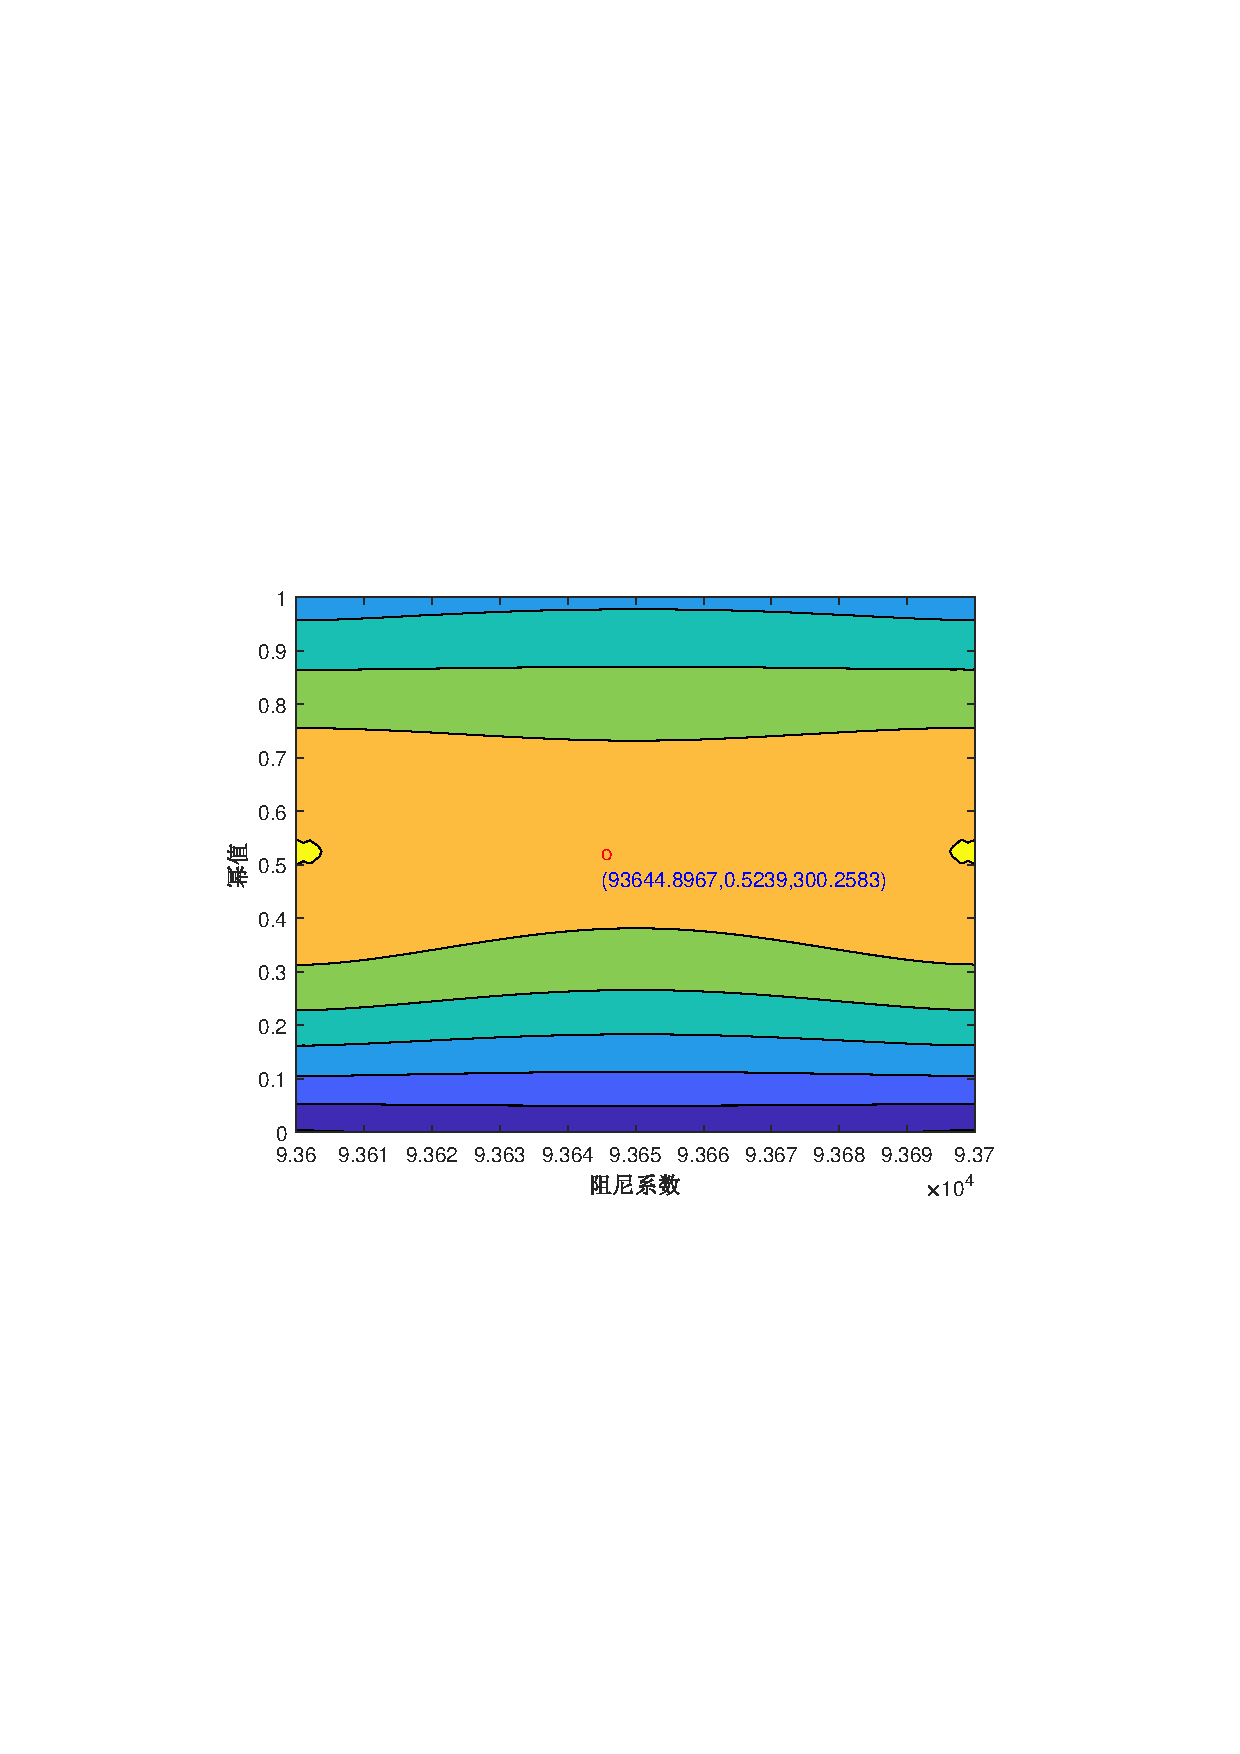
\includegraphics[width=0.8\linewidth]{figures/平面等高线.pdf}
		\end{minipage}
	}
	\subfloat[三维立体图]{
		\begin{minipage}[t]{0.5\textwidth}
			\centering
			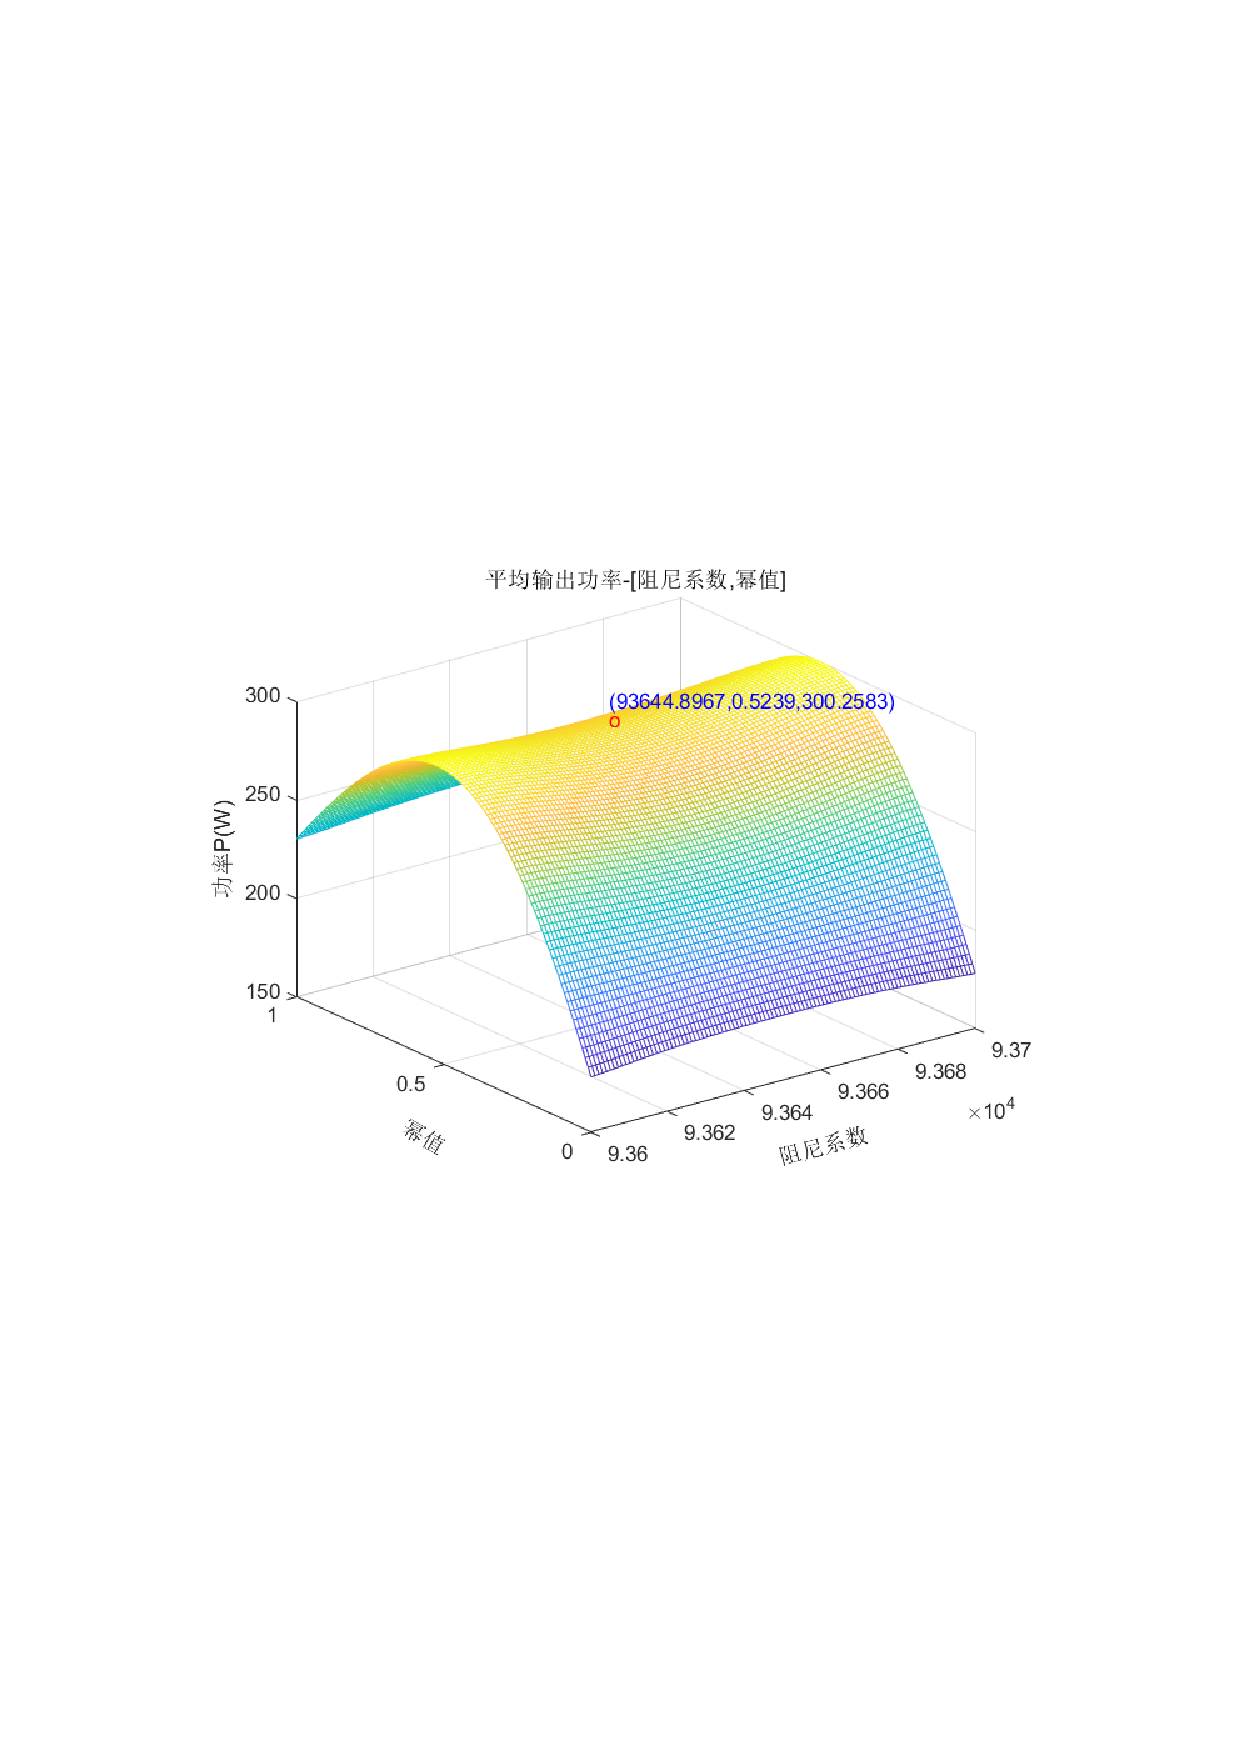
\includegraphics[width=0.8\linewidth]{figures/三维.pdf}
		\end{minipage}
	}
	\caption{遗传算法求解问题二第二小问结果}
\end{figure}


\subsection{问题3模型的建立与求解}

\subsubsection{模型的拆分}

对于问题三,我们很难直接写出浮子与振子的运动方程。根据我们对于浮子在运动过程中o点仅在竖直方向上运动的假设,我们可以分别讨论浮子与振子的转动与平动情况,并通过转动与平动的叠加刻画浮子与振子同时进行垂荡与纵摇的运动状态。

在开始分析之前,为了减少读者不必要的困惑,我们需要简要介绍平面转动参考系非惯性动力学分析与平行轴定理这两个物理分析工具,以减少读者在阅读本文时不必要的困惑。

\textbf{在分析平面转动参考系时},我们有:[3]
$$
	a'=a-\dot{\omega}\times r+\omega^2r-2\omega\times v'
$$
如果质量为m的质点所受到的合外力为F,即$ma=F$,故将上式等号两边同时乘以m得到:
$$
	ma'=F-m\dot{\omega}\times r+m\omega^2r-2m\omega\times v'
$$
式中描述了三种惯性力:$-m\dot{\omega}\times r$,$m\omega^2r$,$-2m\omega\times v$。惯性力$-m\dot{\omega}\times r$由参考系做变角速度引发;惯性力$m\omega^2r$(惯性离心力)由参考系的转动所引起;惯性力$-2m\omega\times v$(科里奥利力)是由于参考系转动与质点对转动参考系又具有相对运动引起的。

\textbf{在分析物体转动惯量时},[3]我们一方面需要确定物体的形状(质量分布情况),另一方面需要确定转动轴的位置。平行轴定理告诉我们物体对某一轴线的转动惯量等于对通过质心的平行轴的转动惯量加上物体质量与两轴间垂直距离平方的乘积,即:
$$
	I = I_c+md^2
$$
式中I是对某轴线的转动惯量,$I_c$是对通过质心的平行轴的转动惯量,d为量平行轴线间的垂直距离。

为了叙述的简便性,在以下分析中使用上述两条规则时不再呈现详细推导过程。我们可以绘制示意图如图10所示。


\begin{figure}[htbp]
	\centering
	\subfloat[浮子转动分析]{
	\begin{minipage}{0.3\linewidth}
		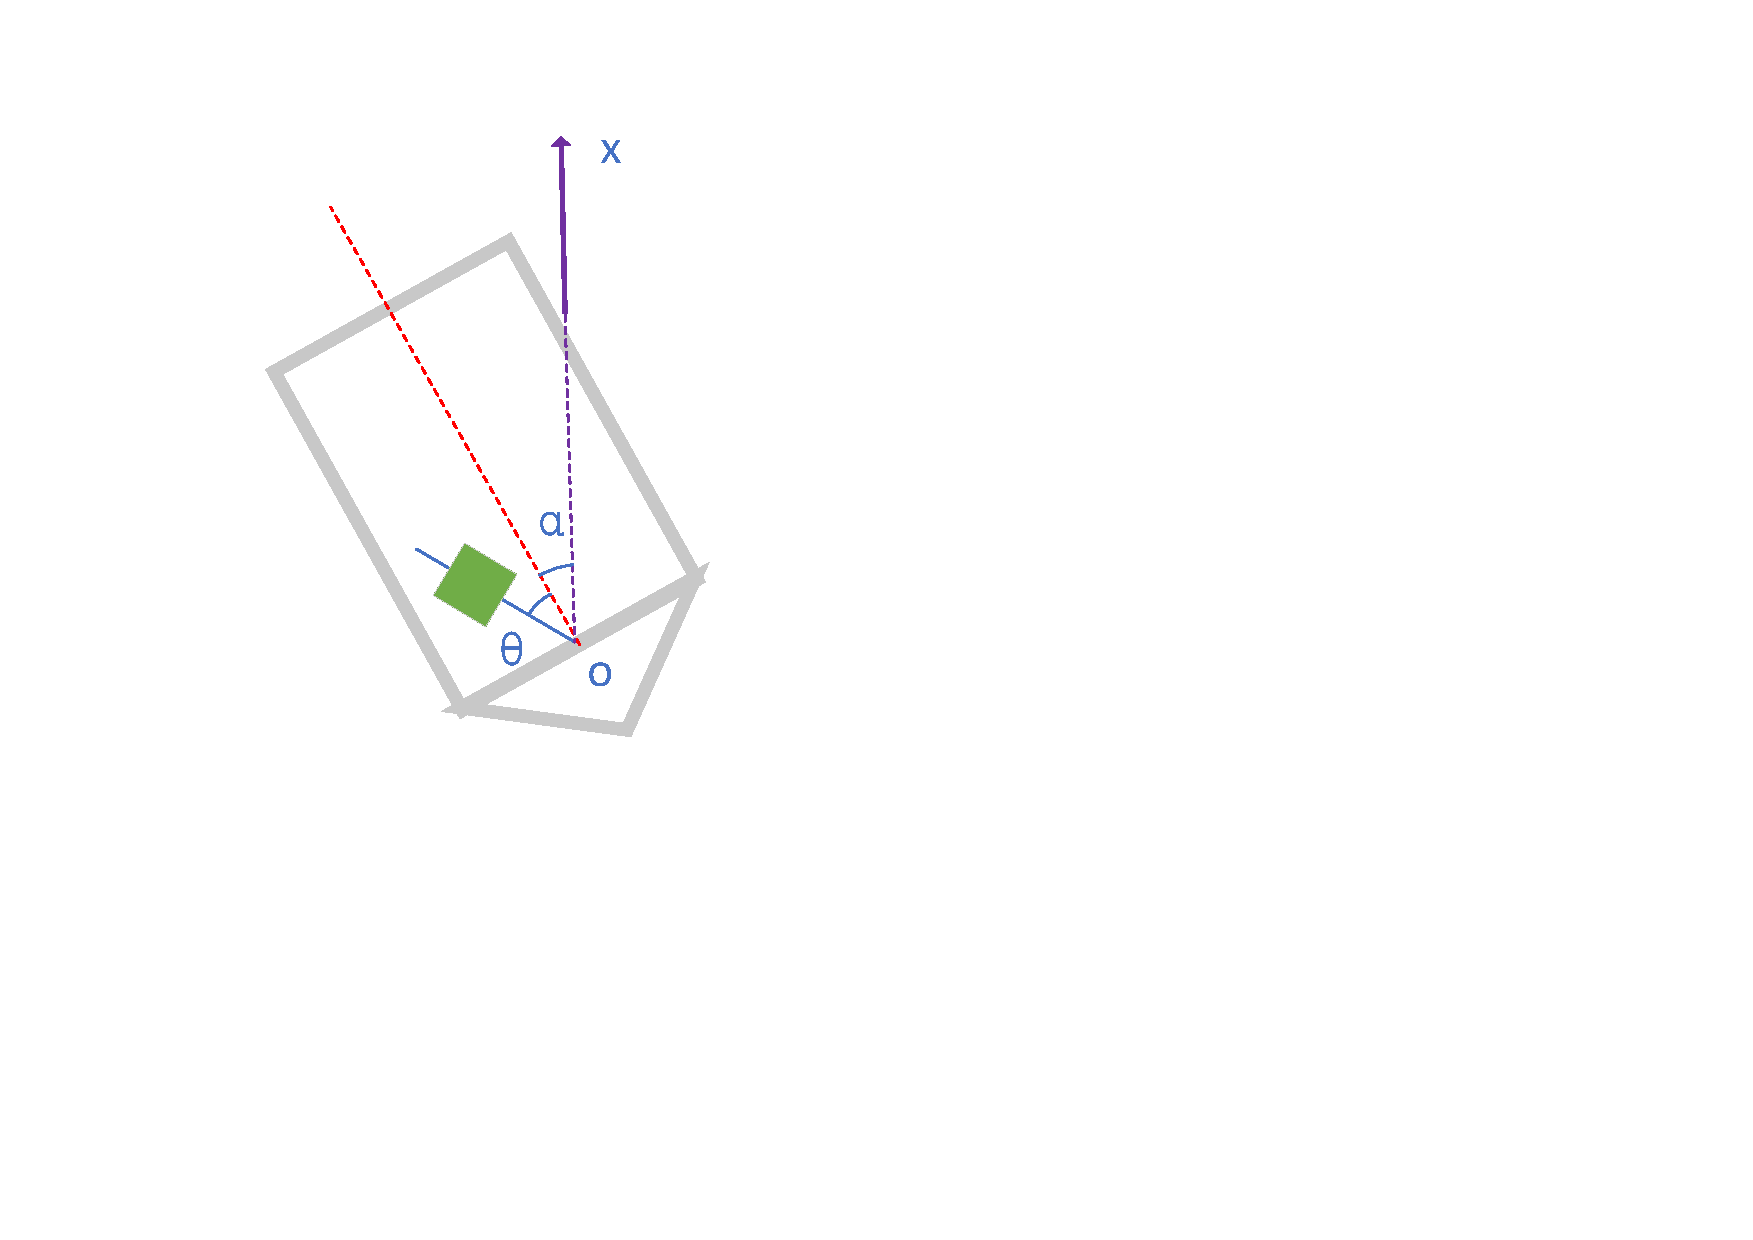
\includegraphics[width=0.9\linewidth]{figures/Q3对浮子转动分析.pdf}
	\end{minipage}
	}
	\subfloat[真实力示意图]{
		\begin{minipage}{0.3\linewidth}
			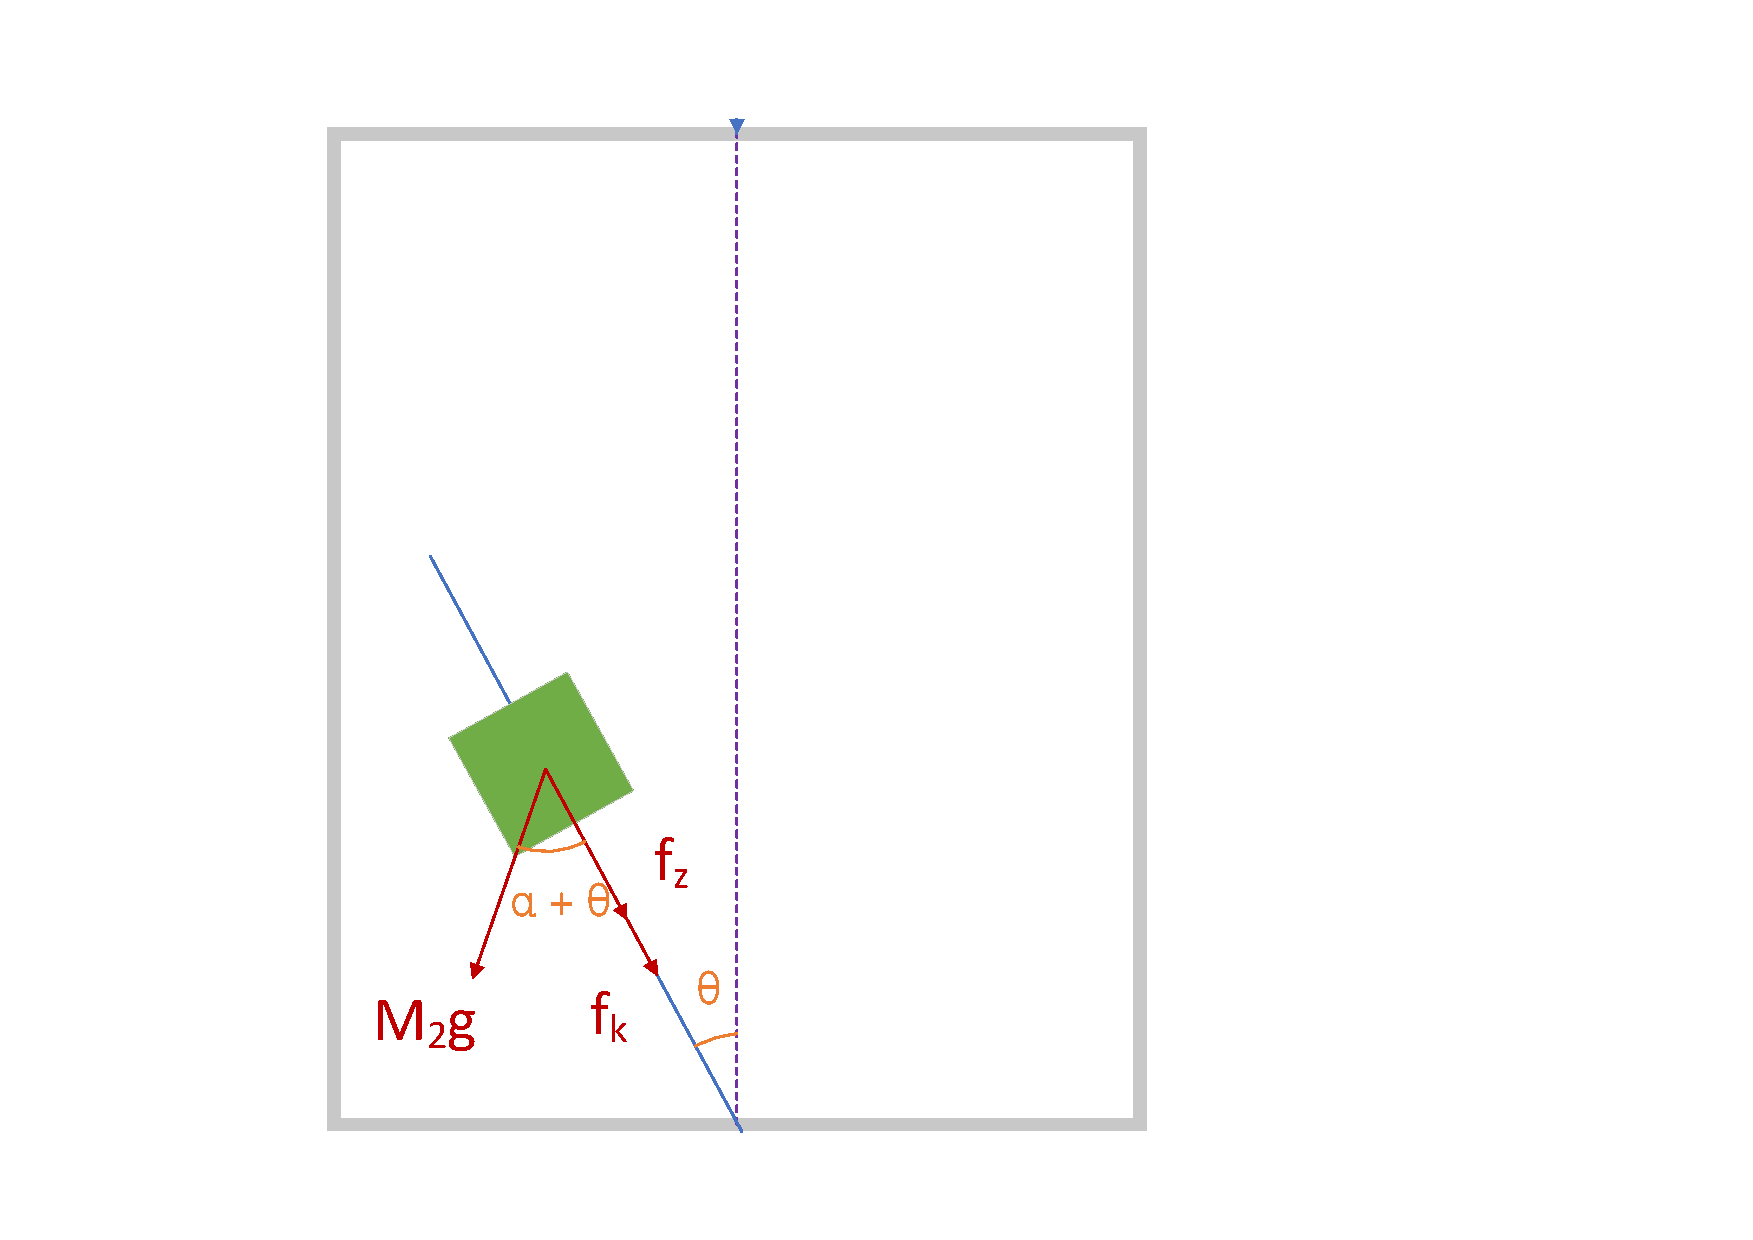
\includegraphics[width=0.9\linewidth]{figures/真实力.pdf}
		\end{minipage}
	}
	\subfloat[惯性力示意图]{
		\begin{minipage}{0.3\linewidth}
			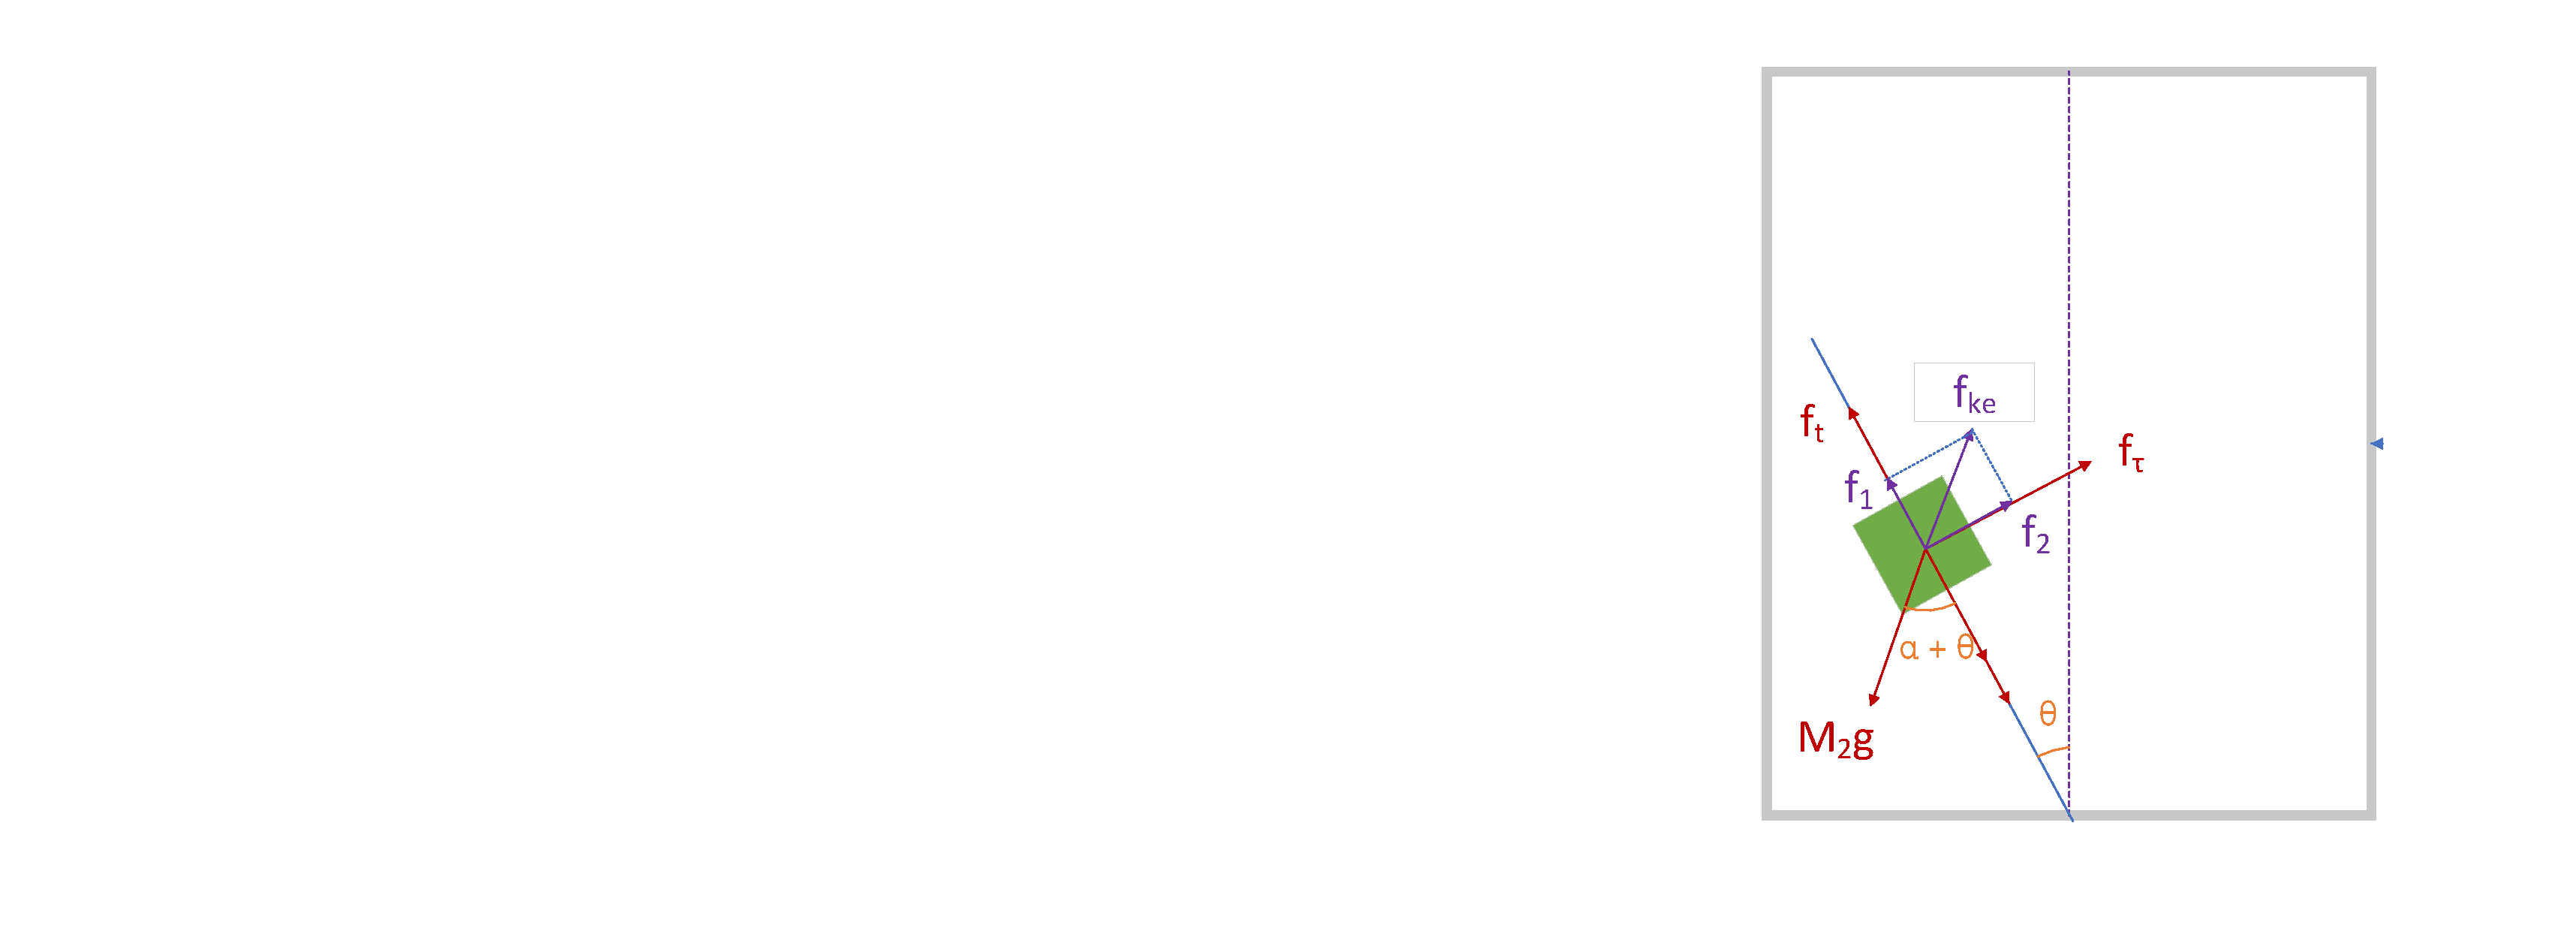
\includegraphics[width=0.9\linewidth]{figures/惯性力.pdf}
		\end{minipage}
	}
\caption{波浪能装置垂荡与纵摇示意图}
\end{figure}

图中$f_t$为惯性离心力;$f_{ke}$为科里奥利力;$f_\tau$为切向惯性力;$f_p$为由浮子平动引起的惯性力;$f_z$为直线阻尼器阻力;$f_k$为弹簧弹力。其中科里奥利力被分解为$f_1$和$f_2$。
$$f_{ke}=2\overrightarrow{v}\times\overrightarrow{\omega}M_2$$
$$f_1 = 2r\dot{\theta}\dot{\alpha}M_2$$
$$f_2 = 2\dot{r}\dot{\alpha}M_2$$

浮子的转动方程为:
\begin{equation}
	\begin{cases}
		I_1\ddot{\alpha} =M_b + M_r + M_\epsilon + M_t \\
		M_r = -I_a\ddot{\alpha} - c_1\dot{\alpha} \\
		M_b = -K_m\alpha \\
		M_\epsilon = L\cos(\omega t) \\
		M_t = K_1\theta + K_2\dot{\theta}
		
	\end{cases}
\end{equation}
式中$I_1$为浮子对轴的转动惯量,数值为16882;$M_r$为辐射力矩,包括附加惯性力矩和兴波阻尼力矩;$M_b$为静水恢复力矩;$M_\epsilon$为波浪激励力矩;$M_t$为扭转弹簧与旋转阻尼力矩;$I_a$为骨架转动惯量;$K_1$为扭转弹簧刚度;$K_2$为旋转阻尼弹性系数;$c_1$为纵摇兴波阻尼系数。




振子转动方程为:(此时我们以浮子为参考系建立极坐标系,振子质心位置可以表示为$(r,\theta)$)
\begin{equation}
	\begin{cases}
		I_2\ddot{\theta} = M_z - M_t + M_\tau + M_k + M_p \\
		M_z = M_2 g r \sin\theta \\
		-M_t = -K_1\theta + -K_2\dot{\theta} \\
		M_\tau = f_\tau r = -\ddot{\alpha}rM_2r \\
		M_k = f_2 r = -2\dot{\alpha}\dot{r}M_2r \\
		M_p = f_p r\sin\theta = M_2\ddot{x}r\sin\theta \\
		
		
	\end{cases}
\end{equation}

式中$M_z$为重力力矩;$M_t$为扭转弹簧与旋转阻尼力矩;$M_\tau$为转动引起的切向惯性力矩;$M_k$为科氏惯性力矩;$M_p$为平动引起的力矩;$f_\tau=-\ddot{\alpha}rM_2$为惯性切向力;$f_2=-2\dot{\alpha}\dot{r}M_2$为科里奥利力沿切向的分力;$f_p = M_2\ddot{x}$为由浮子平动所引起的惯性力。$I_2$为$M_2$的转动惯量,应用平行轴定理和微积分计算后得到:
\begin{equation}
	I_2 = (\frac{1}{2}R_2^2h+\frac{1}{12}h^3+\frac{1}{4}R_2^3 + \frac{1}{4}R_2h^2)\frac{M_2}{R_2+h}+M_2R_2^2
\end{equation}


浮子平动方程为:
\begin{equation}
	\begin{cases}
		M_1\ddot{x} = f_h +f_T+f_z\\
		f_h = f_b + f_r + f_\epsilon = -\rho g\pi xR_1^2-M_a\ddot{x}-C_{rd}\dot{x}+f\cos\omega t\\
		f_T = K_t(r-L)\cos(\alpha+\theta) \\
		f_z = K_z\dot{r}\cos(\alpha+\theta)
		
	\end{cases}
\end{equation}
式中各变量含义与问题一模型中同名变量相同

振子径向运动方程为:

\begin{equation}
	\begin{cases}
		M_2\ddot{r} = f_t +M_2g\cos\theta+f_p\cos\theta+F_z+f_1\\
		f_t = \dot{\alpha}^2 r M_2 \\
		f_p = -\ddot{x}M_2 \\
		F_z = -K_T(r-L)-K_z\dot{r}
		f_1=2r\dot{\theta}\dot{\alpha}M_2
	\end{cases}
\end{equation}
式中$f_p$为由浮子平动引起的惯性力;$f_t$为惯性离心力;$F_z$为弹簧与阻尼器的合力;$f_1$为科里奥利力沿径向方向的分力。惯性切向力$f_\tau$与科里奥利力$f_k$与振子沿中轴平动方向垂直,在此处无作用。

\subsubsection{模型的建立}

综合上述四种情况,我们可以得到一个由四个二元二阶微分方程组成的方程组。

\begin{equation}
	\begin{cases}
		I_1\ddot{\alpha} = -K_m\alpha-I_a\alpha-c_1\dot{\alpha} + L\cos\omega t + K_1\theta + K_2\theta \\
		I_2\ddot{\theta}  = M_2gr\sin\theta-K_1\theta-K_2\dot{\theta}-\ddot{\alpha}r^2M_2-2\dot{\alpha}\dot{r}M_2-M_2\ddot{x}r\sin\theta \\
		M_1\ddot{x} = -\rho g\pi x-M_a\ddot{x}-C_{rd}\dot{x}+f\cos\omega t+K_T(r-L_0)\cos(\alpha+\theta) + K_z\dot{r}\cos(\alpha+\theta) \\
		M_2\ddot{r} = \dot{\alpha}rM_2-M_2g\cos\theta - \ddot{x}M_2\cos\theta - K_T(r-L_0)-K_z\dot{r}+2r\dot{\theta}\dot{\alpha}M_2
	\end{cases}
\end{equation}

\subsubsection{模型的求解}

问题三所采用的求解工具与问题一相同,但在细节处理上有一些差别。通过求解方程组我们可以直接求得$x(t)$,$\dot{x}(t)$,$\alpha(t)$, $\dot{\alpha}(t)$,即可以直接求解出浮子的各项参数。对于振子,由于在建立方程时以浮子为坐标系,所以振子实际的计算结果应该从浮子参考系更换到地面参考系之中。经过计算后,更换方程如表1所示。

\begin{table}[!ht]
	\centering
	\caption{方程求解结果与题目所求结果转换关系}
	\begin{tabular}{|c|c|c|c|c|} \hline
		& 垂荡位移 & 速度 & 纵摇角位移 & 角速度 \\ \hline
		浮子 & $x(t)$ & $\dot{x}(t)$ & $\alpha(t)$ & $\dot{\alpha}(t)$ \\ \hline
		振子 & $x(t)+r(t)\cos(\theta+\alpha)$ & $\dot{x}(t)+\dot{r}\cos(\theta+\alpha) - r\sin(\theta+\alpha)(\dot{\theta}+\dot{\alpha})$ & $\theta(t)+\alpha(t)$ & $\dot{\theta}(t)+\dot{\alpha}(t)$ \\ \hline
	\end{tabular}
\end{table}

我们使用基于matlab的ode45方法将方程求解过后 ,得出了问题三中浮子与振子在10 s、
20 s、40 s、60 s、100 s 时的垂荡位移与速度和纵摇角位移与角速度如图11 。详细结果请参考“支撑材料”文件夹->“T3”文件夹->result3.xlsx.

\begin{figure}[h]
	\centering
	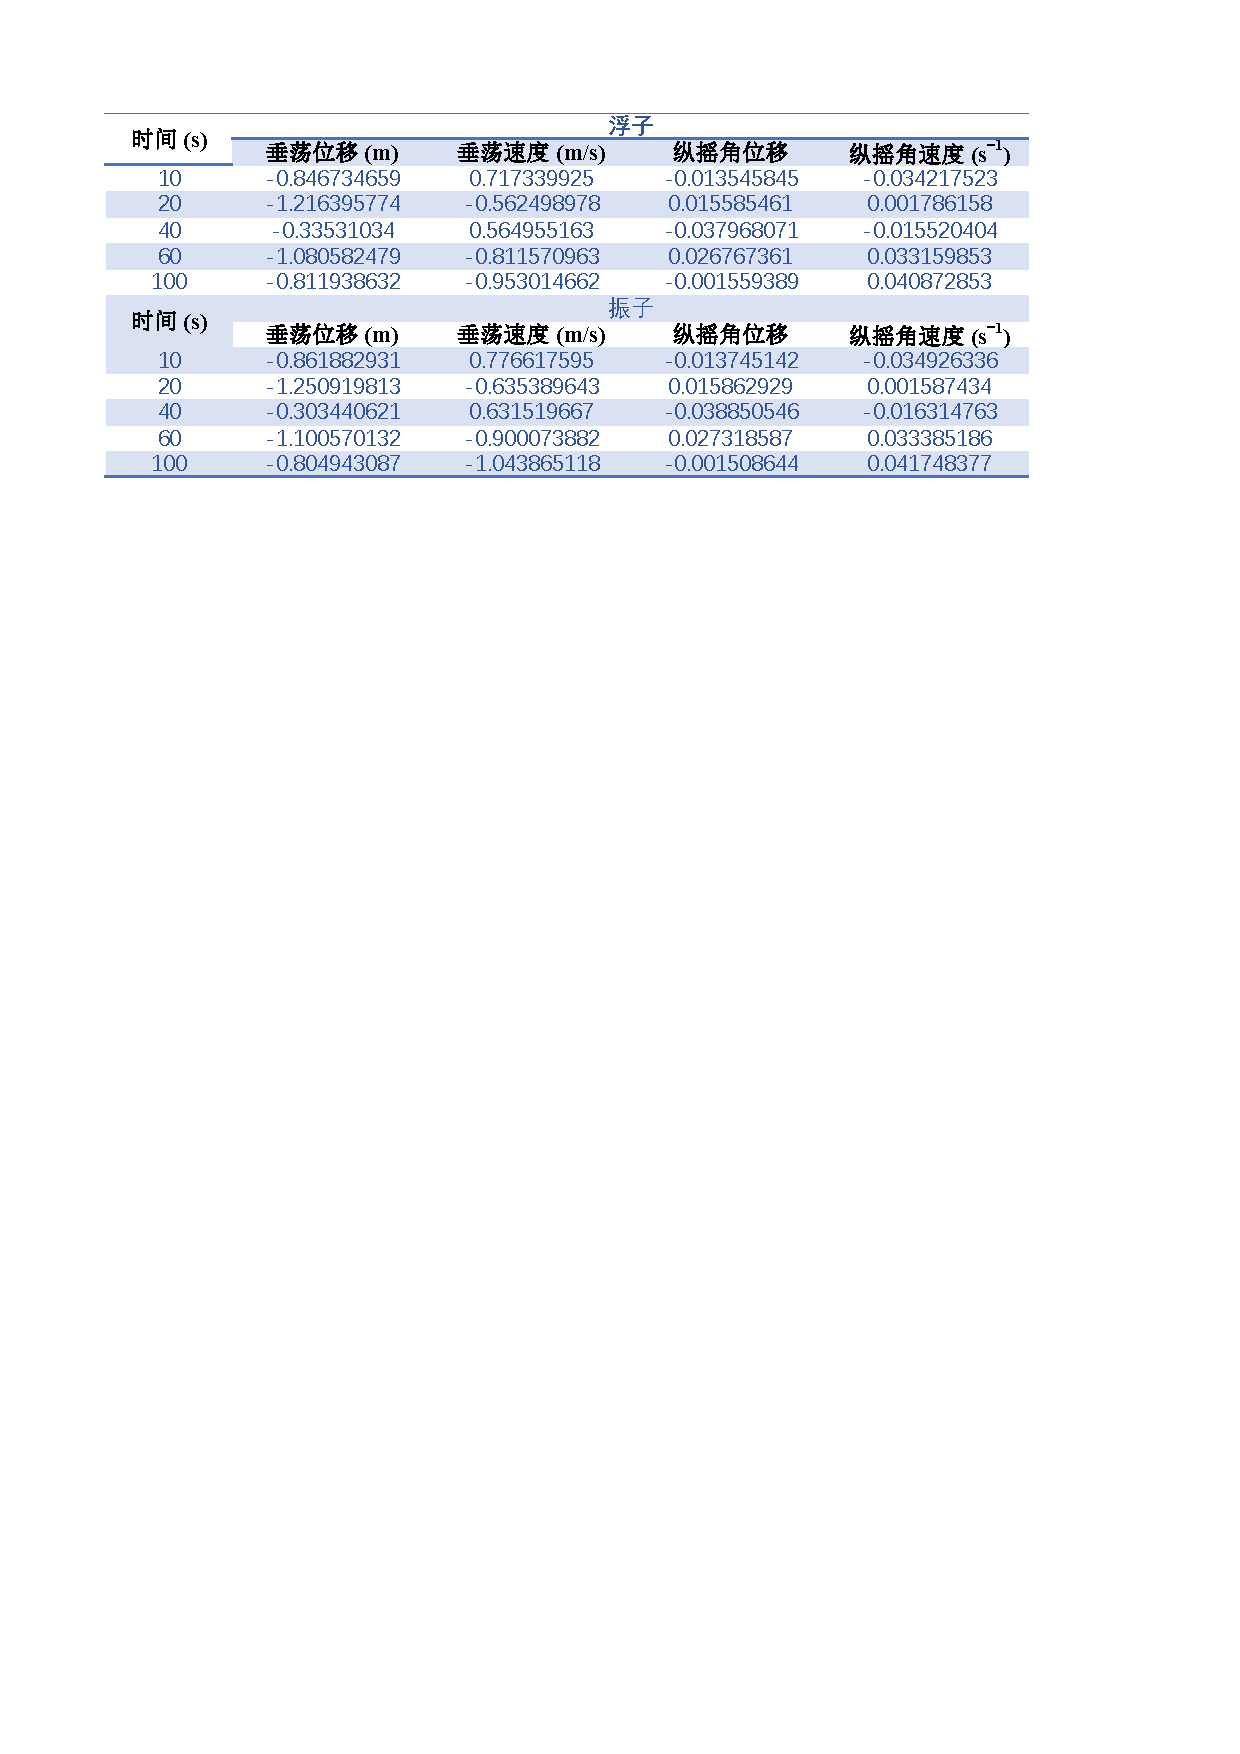
\includegraphics[width=0.7\linewidth]{figures/result3.pdf}
	\caption[]{阻尼系数恒定时模型计算结果}
	\label{fig:result1-1}
\end{figure}

将计算结果通过matlab进行可视化表示,我们得到了如图12的曲线。从曲线图中我们发现浮子的角位移非常小,且旋转阻尼器的输出功率远小于直线阻尼器的输出功率。但同时我们也发现纵摇的加入使得直线阻尼器的输出功率较单纯的垂荡运动功率增加了一倍左右。经过分析,我们猜测原因可能是考虑纵摇的情况后,在振子的运动轨道中轴的径向上多了科里奥利力和惯性离心力。由于这两个惯性力的作用,振子相对于浮子的径向振动振幅增大,导致其输出功率显著上升。

\begin{figure}[htbp]
	\centering
	\begin{minipage}{0.45\linewidth}
		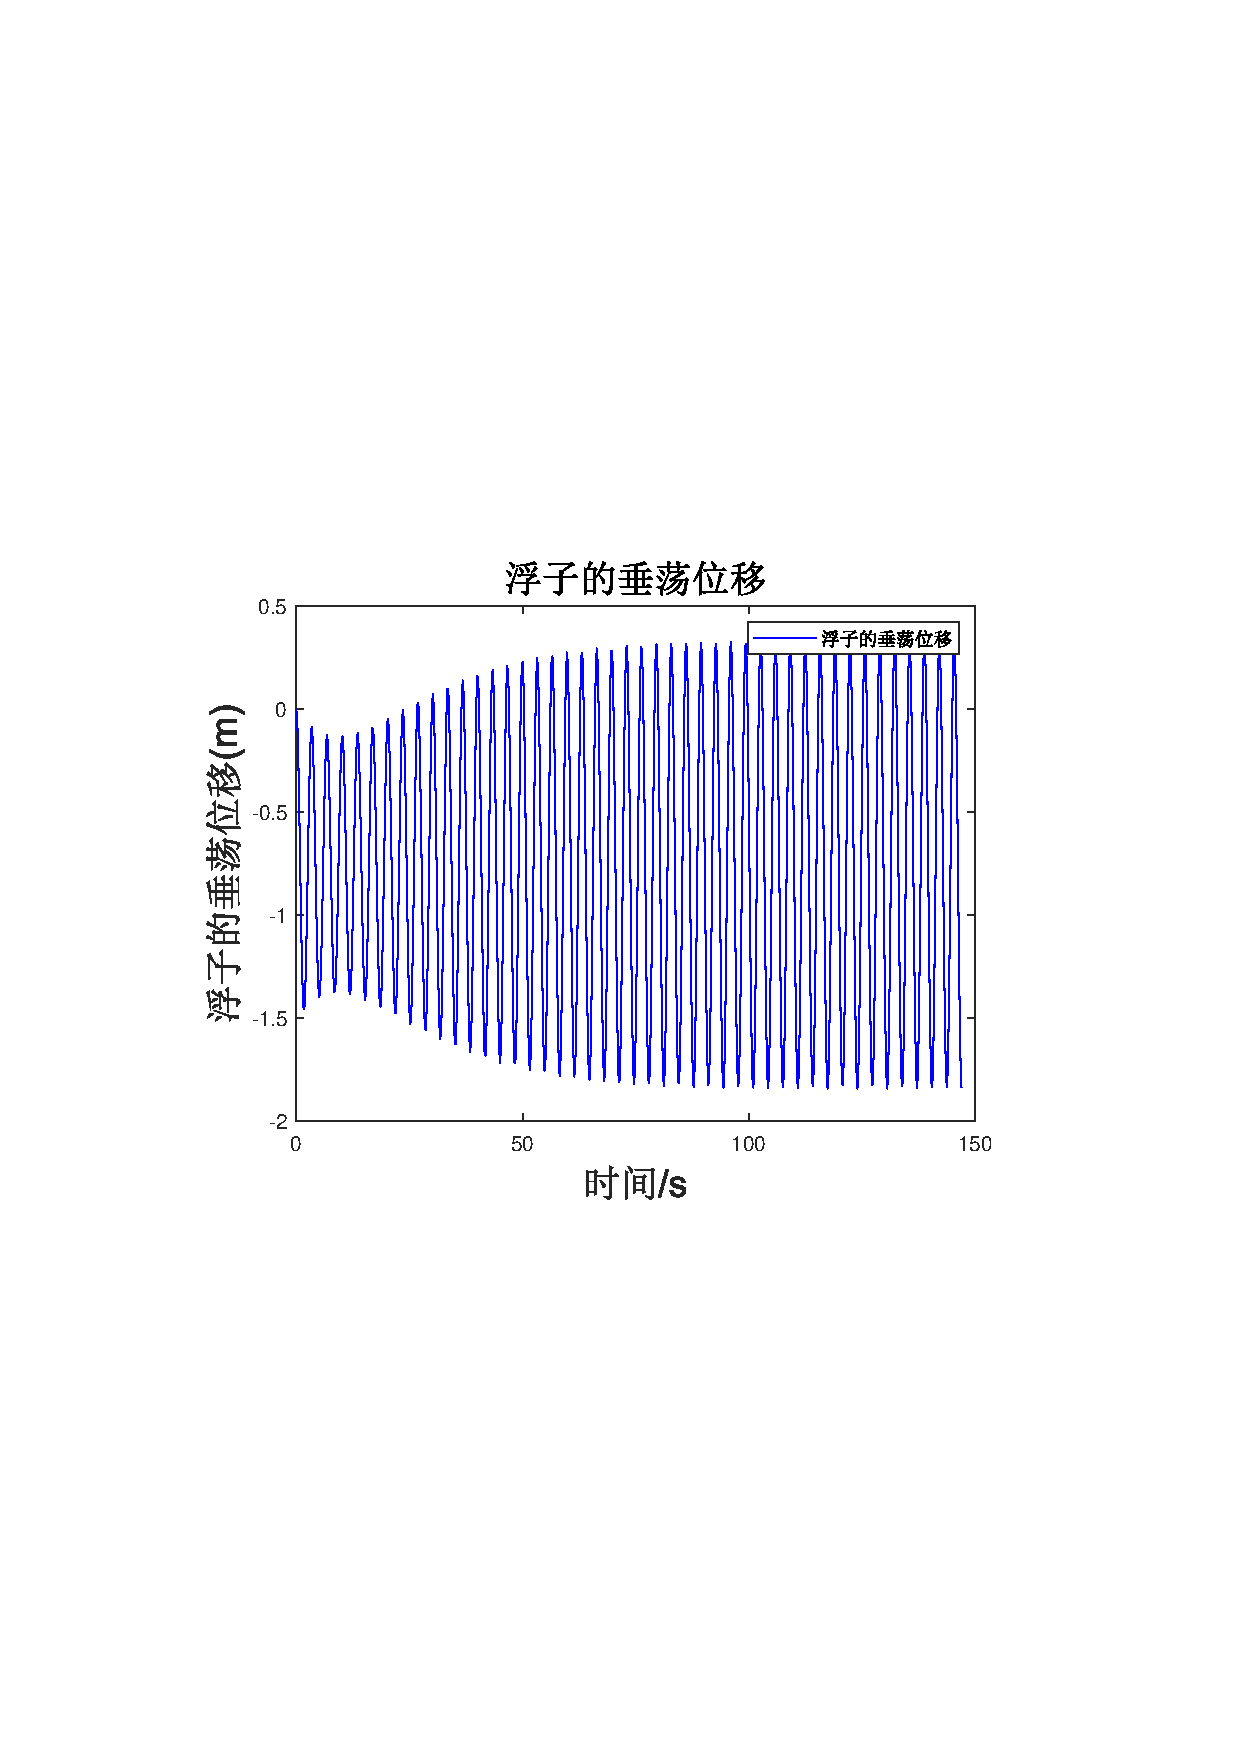
\includegraphics[width=0.9\linewidth]{figures/浮子垂荡位移.pdf}
	\end{minipage}
	\begin{minipage}{0.45\linewidth}
		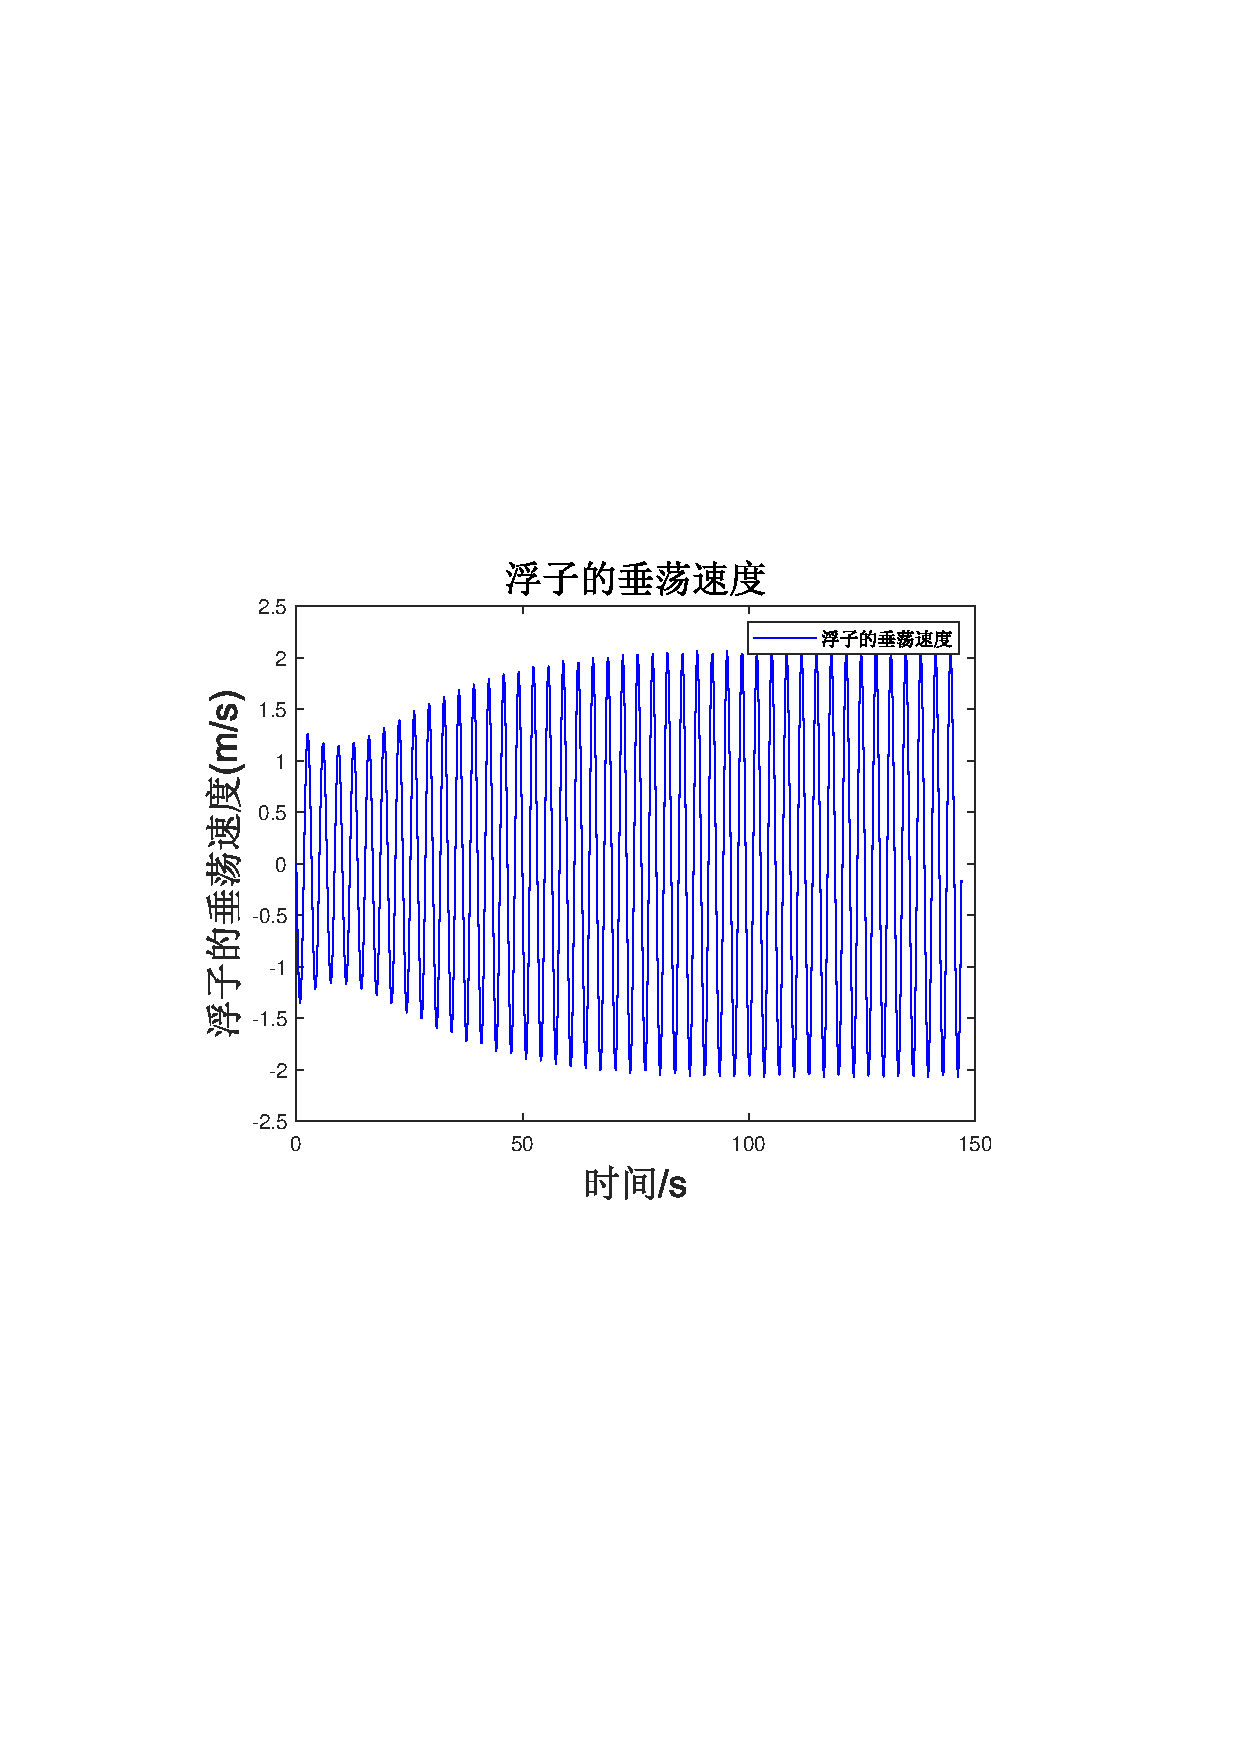
\includegraphics[width=0.9\linewidth]{figures/浮子的垂荡速度.pdf}
	\end{minipage}
	%\qquad
	%让图片换行,
	\begin{minipage}{0.45\linewidth}
		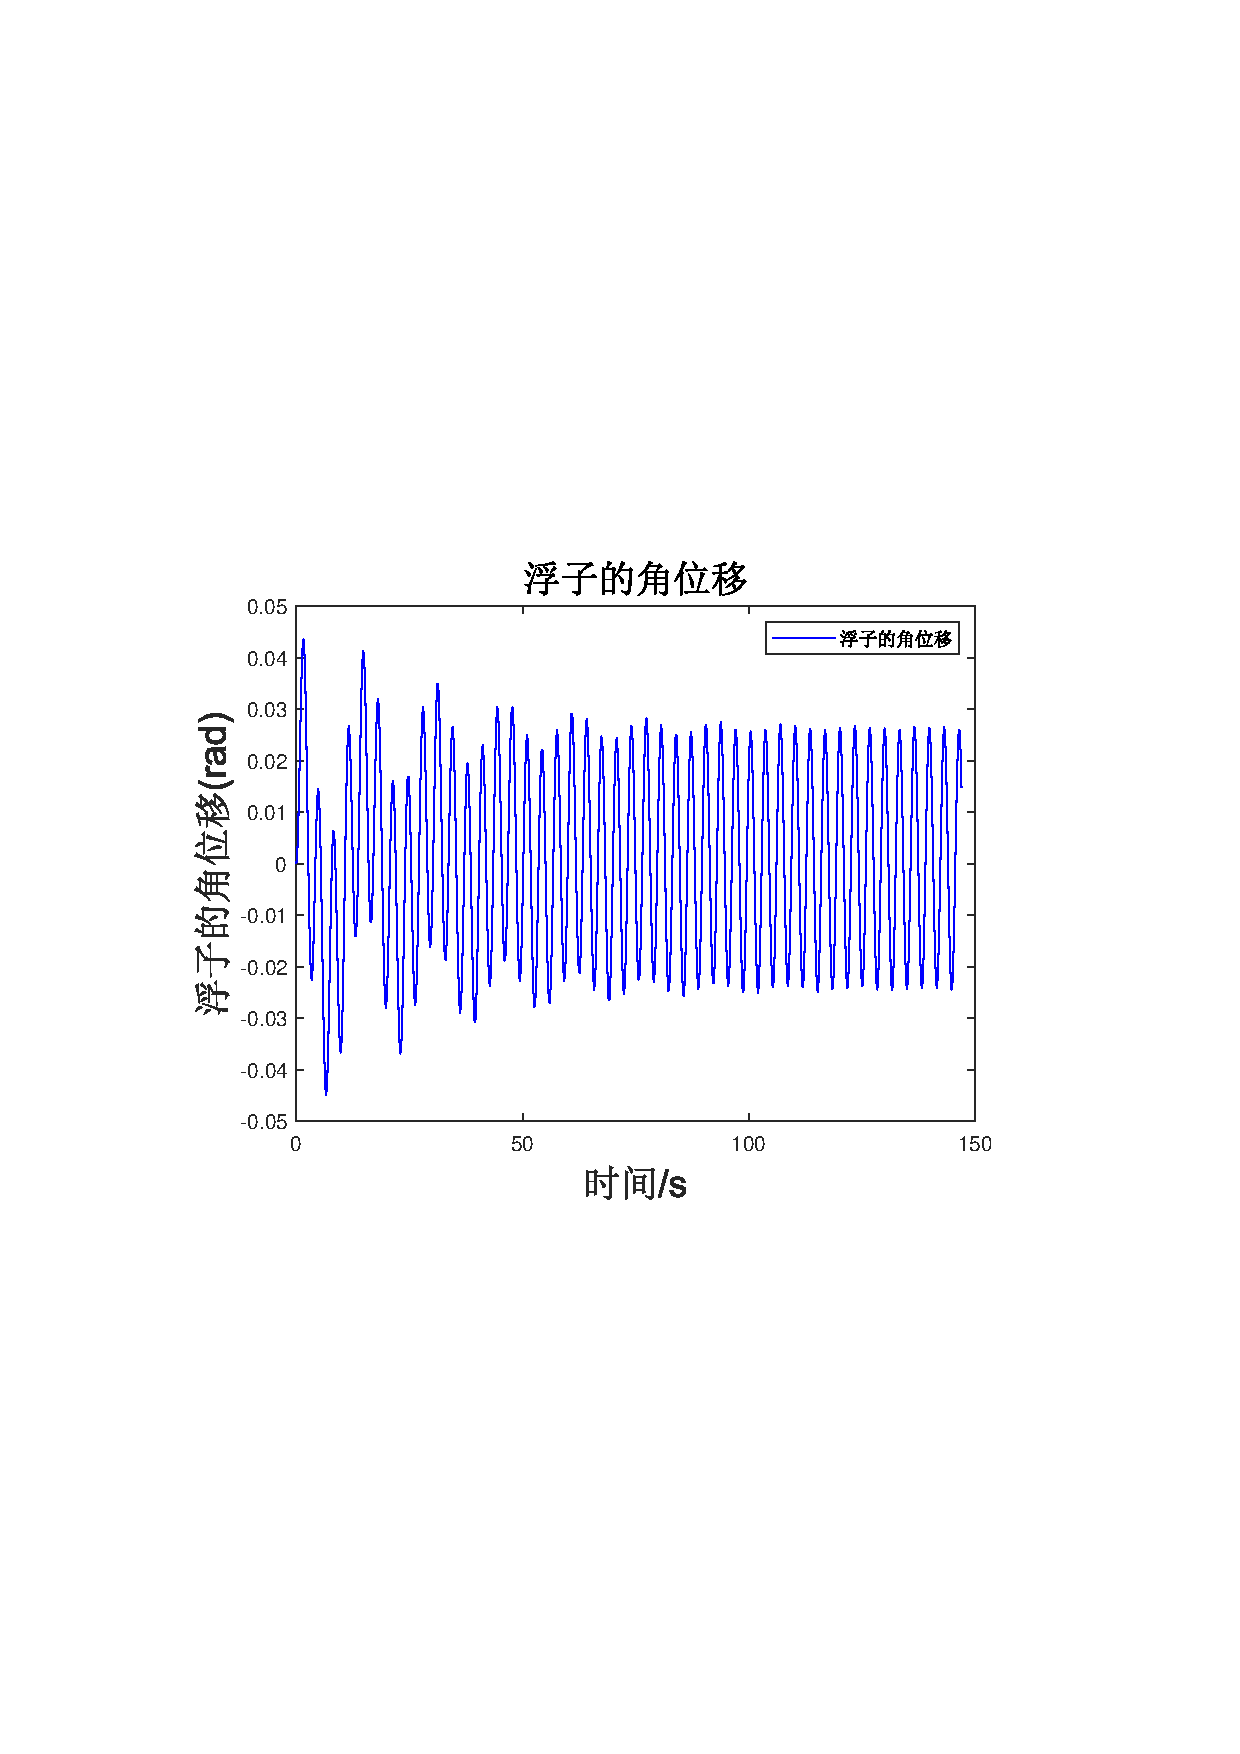
\includegraphics[width=0.9\linewidth]{figures/浮子的角位移.pdf}
	\end{minipage}
	\begin{minipage}{0.45\linewidth}
		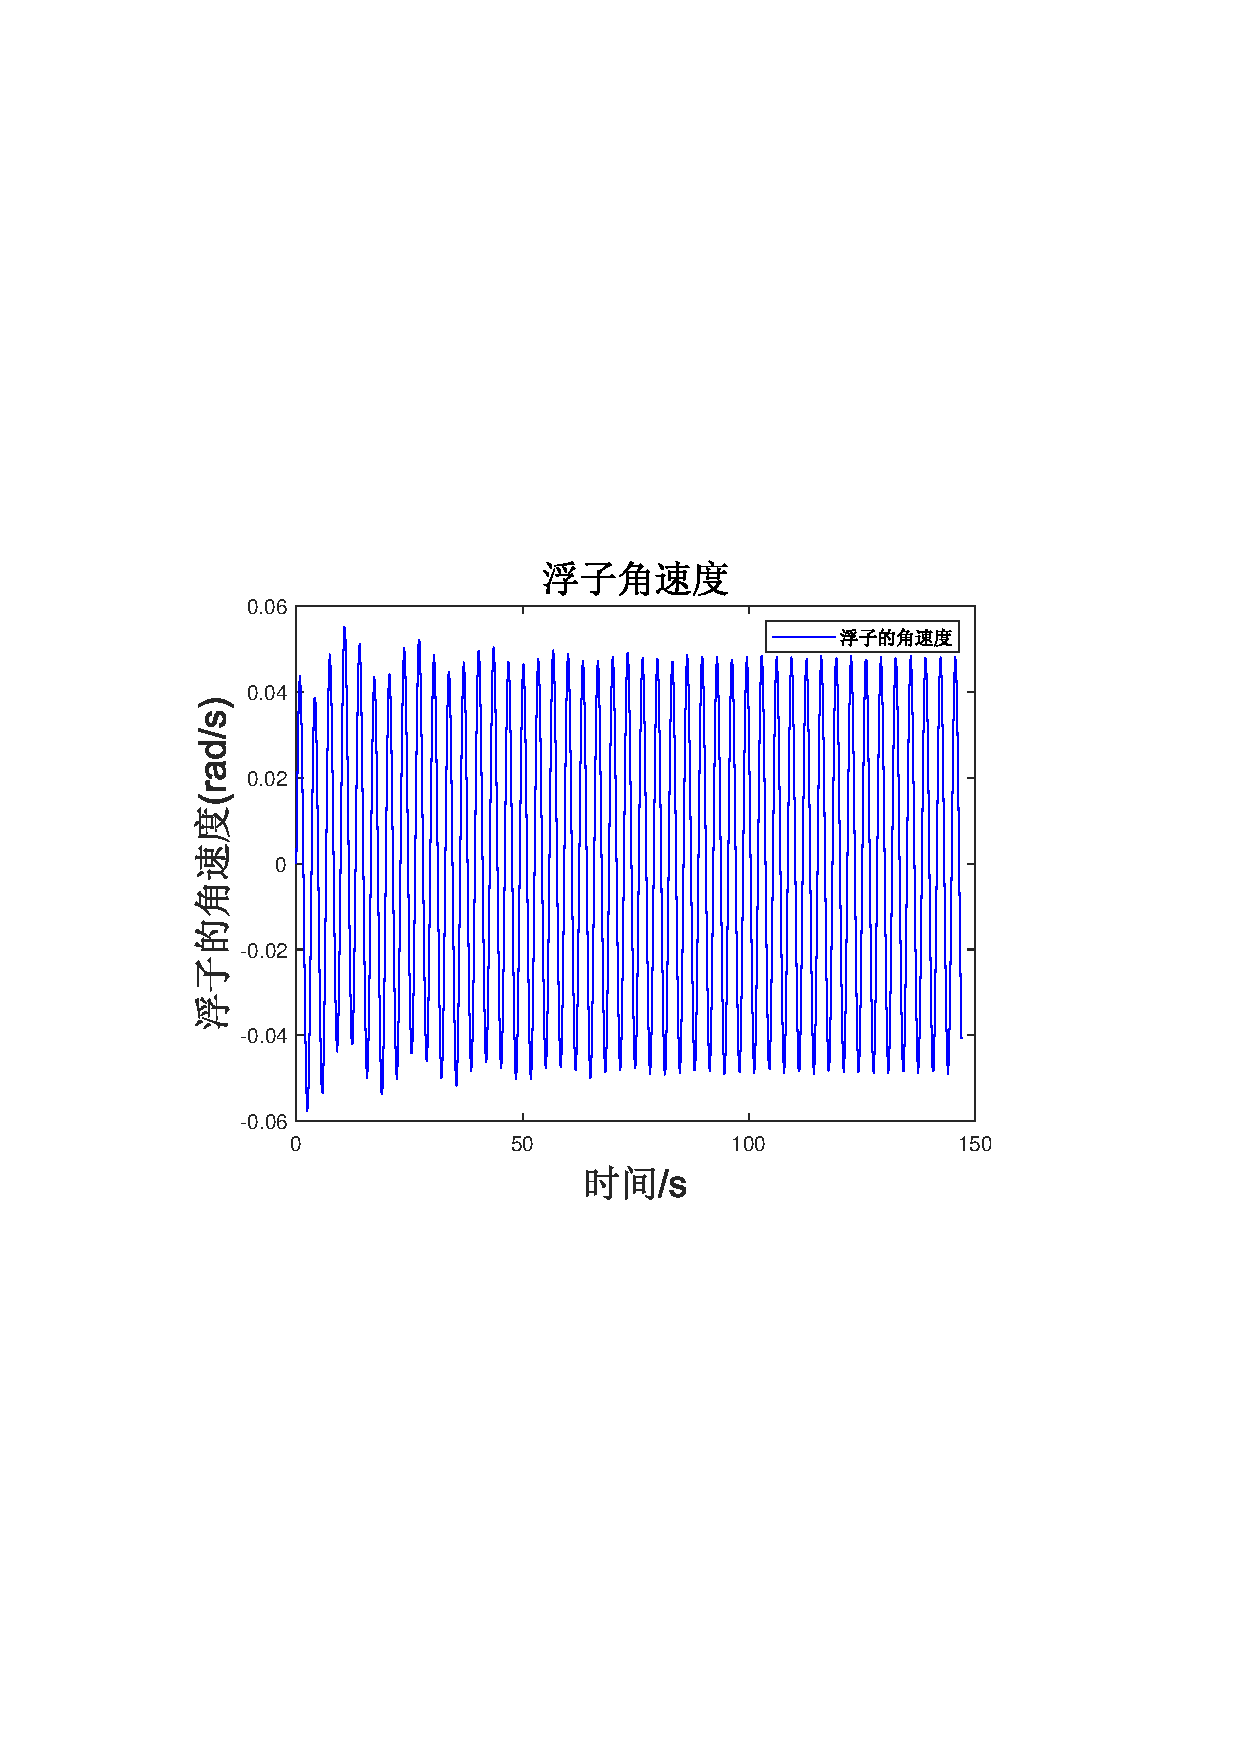
\includegraphics[width=0.9\linewidth]{figures/浮子角速度.pdf}
	\end{minipage}
	\begin{minipage}{0.45\linewidth}
		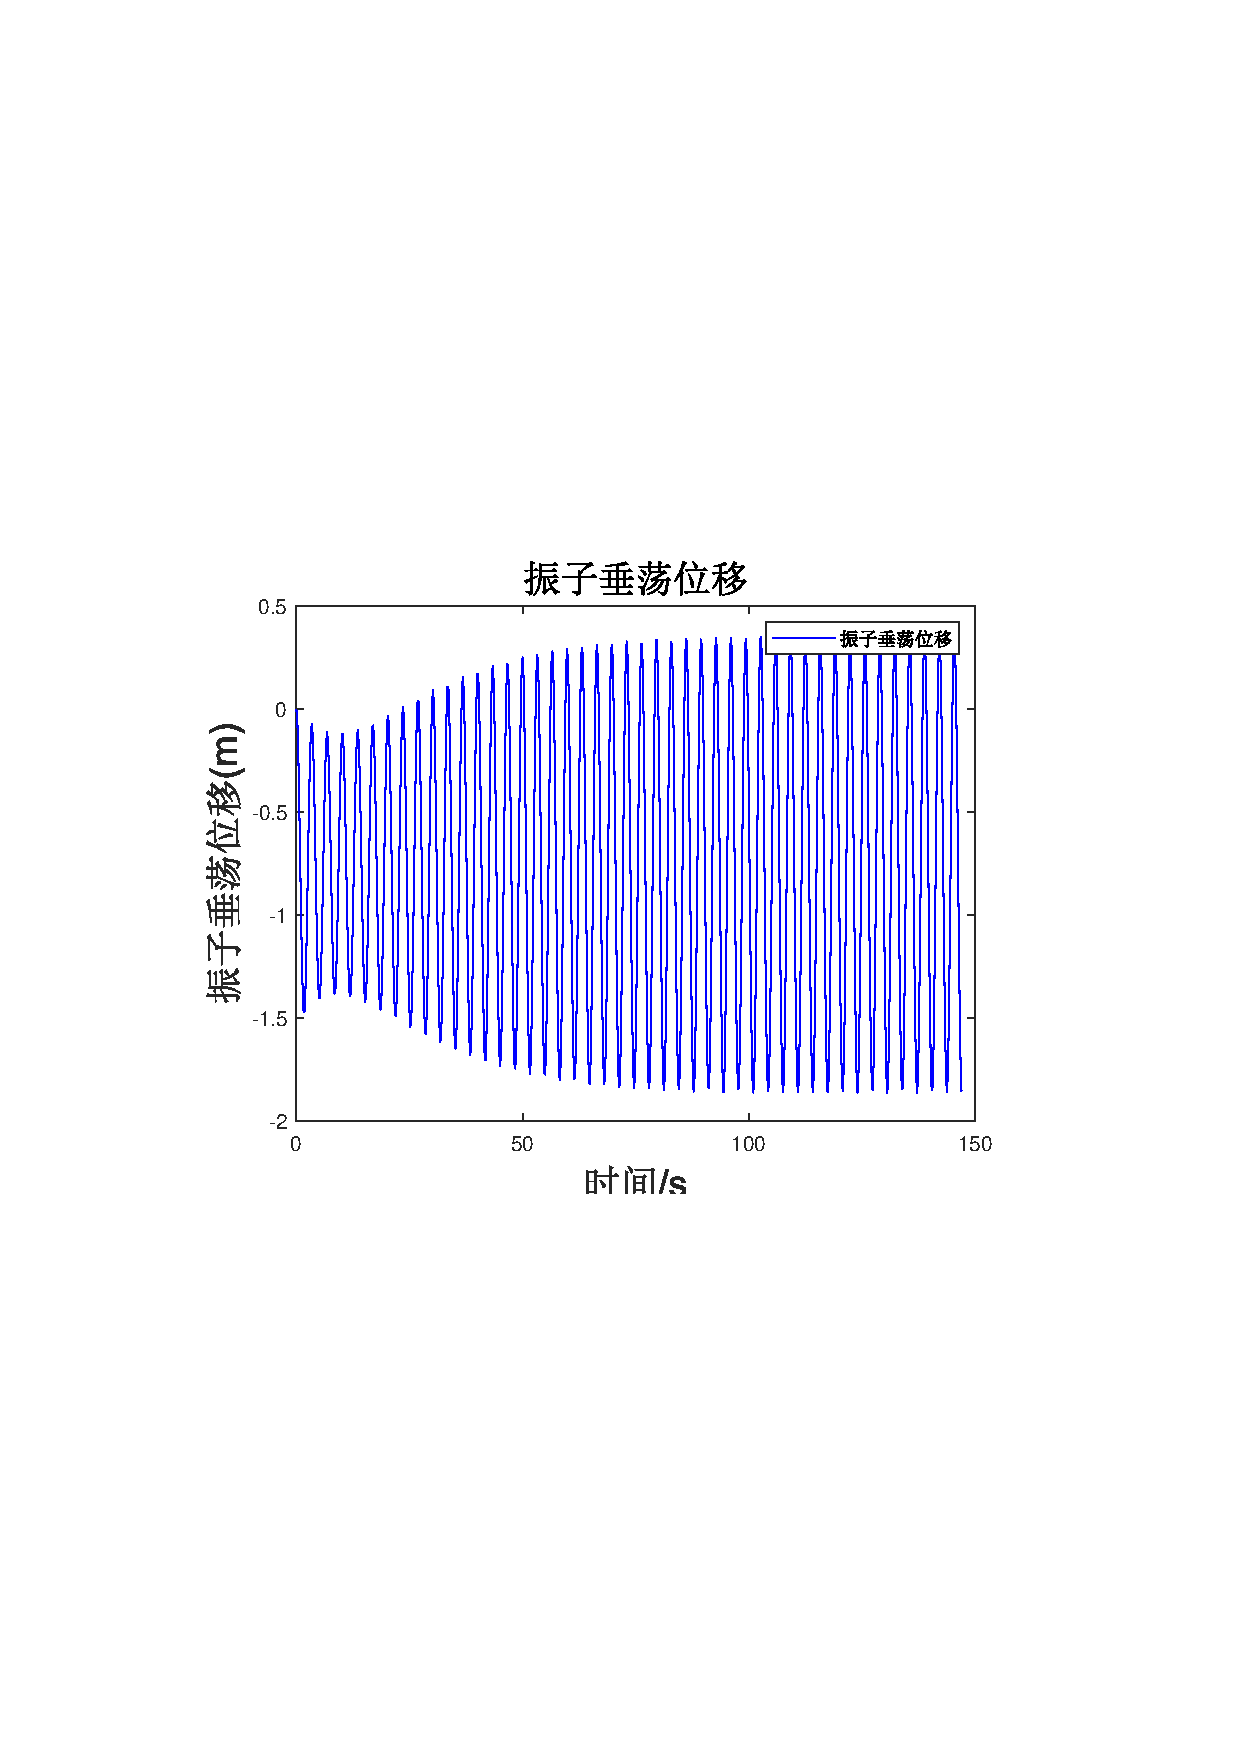
\includegraphics[width=0.9\linewidth]{figures/振子垂荡位移.pdf}
	\end{minipage}
	\begin{minipage}{0.45\linewidth}
		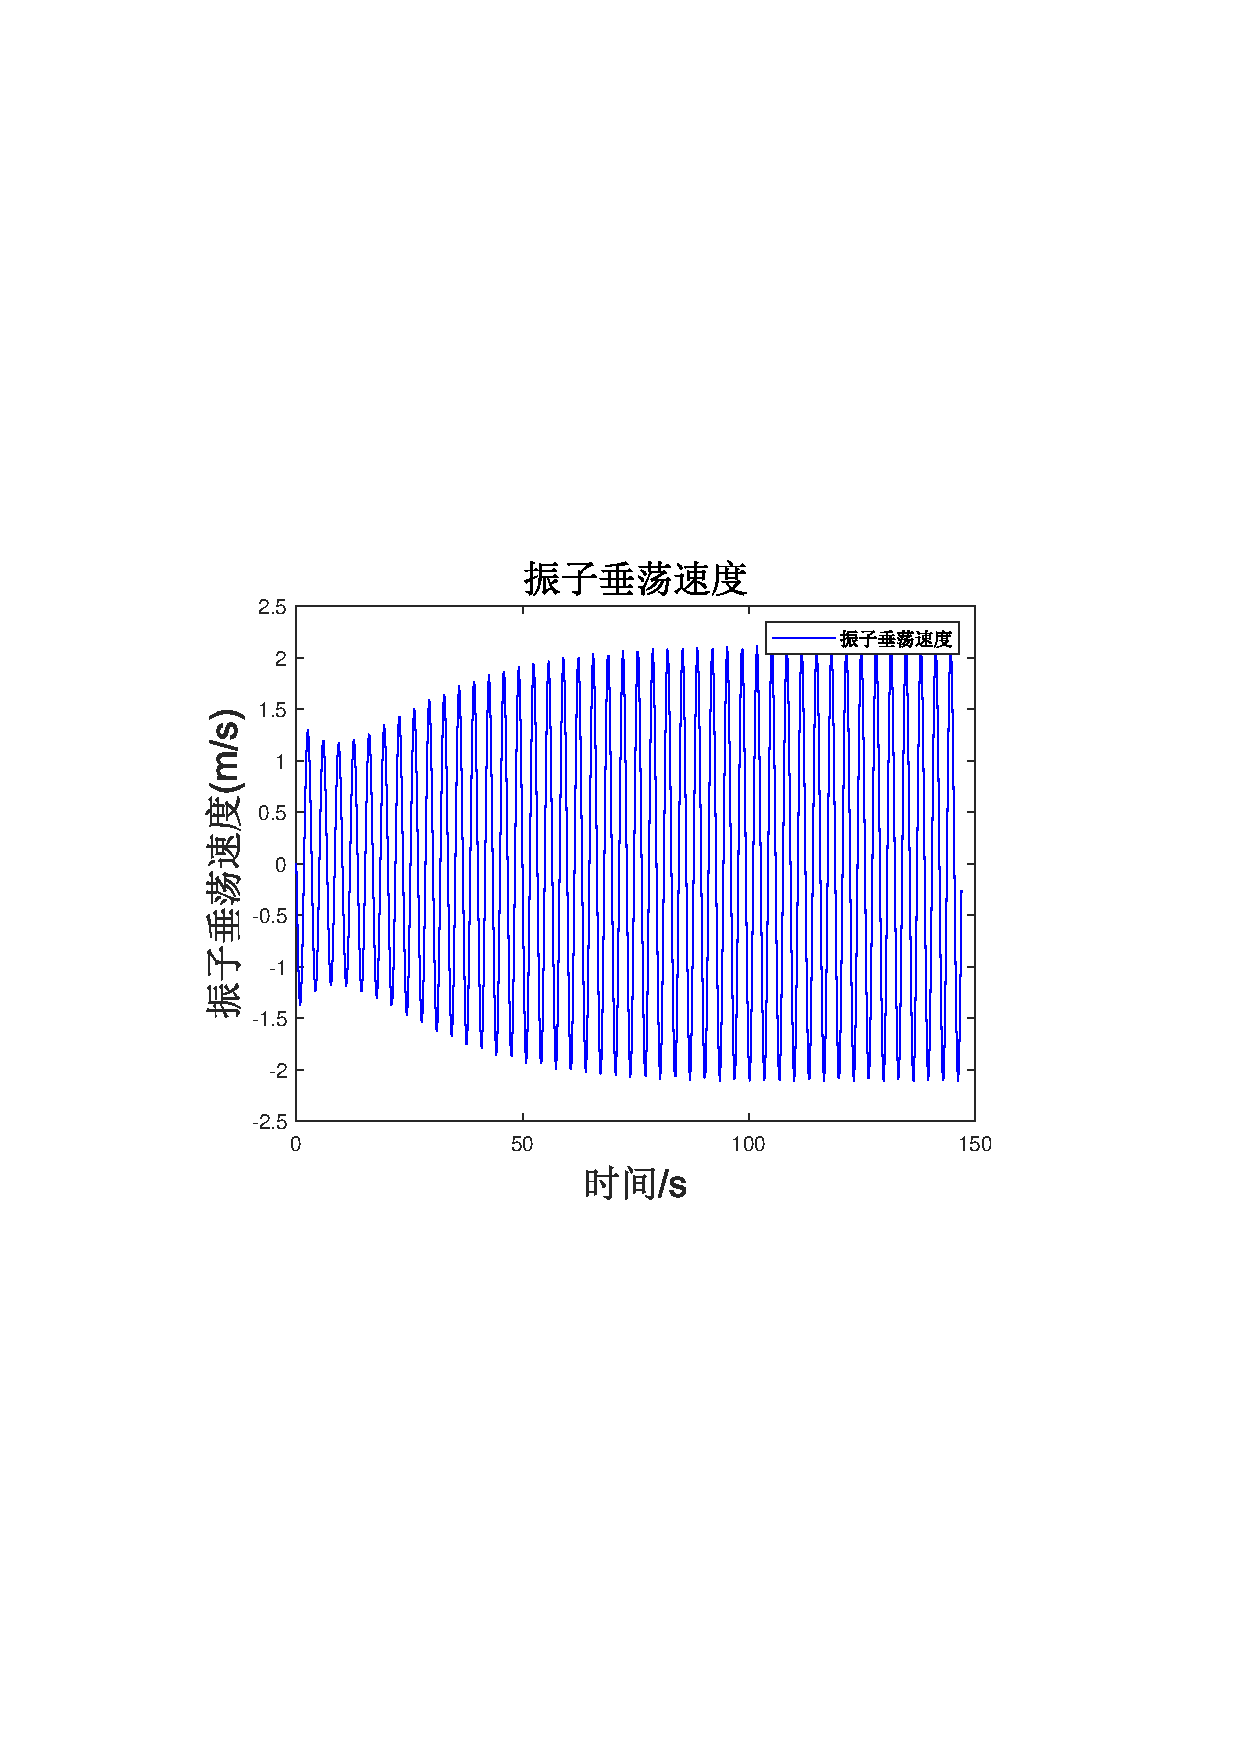
\includegraphics[width=0.9\linewidth]{figures/振子垂荡速度.pdf}
	\end{minipage}
	%\qquad
	%让图片换行,
	\begin{minipage}{0.45\linewidth}
		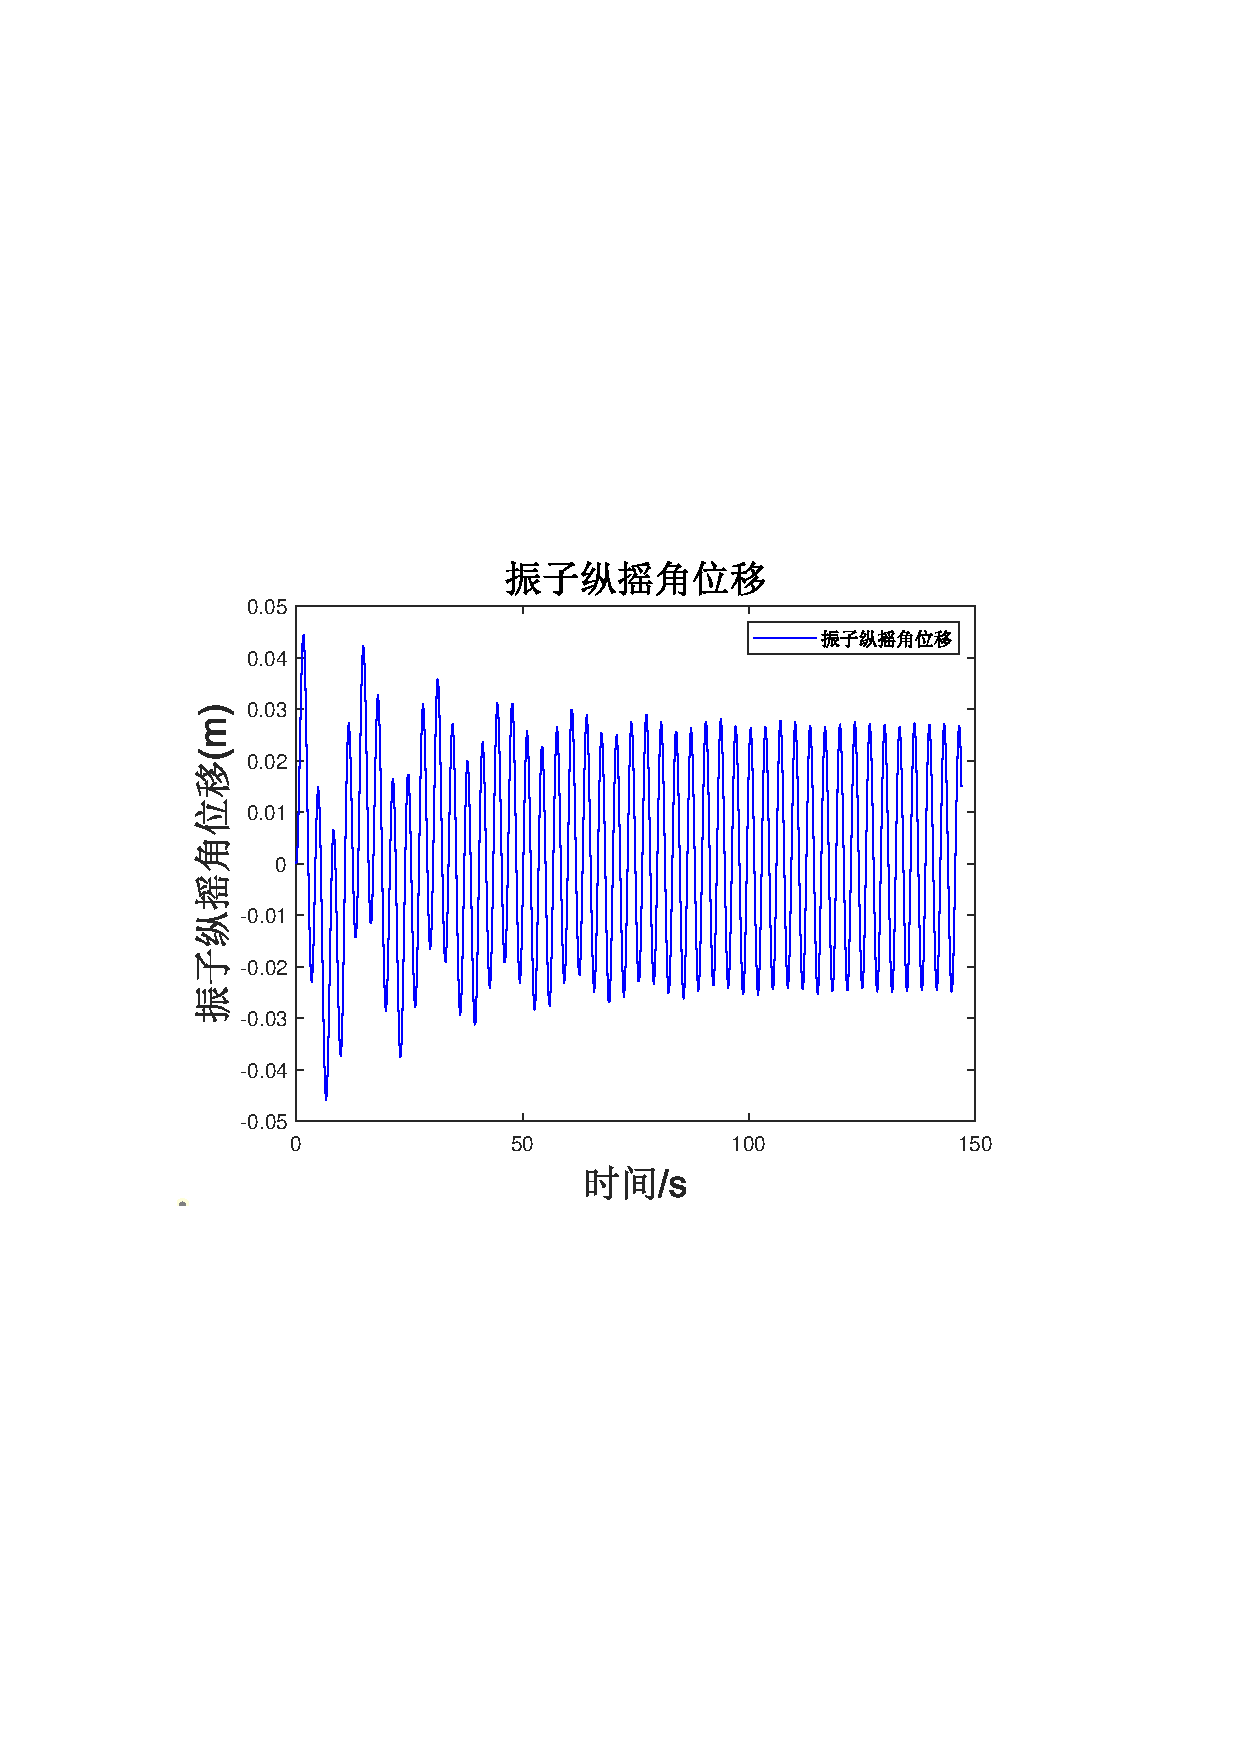
\includegraphics[width=0.9\linewidth]{figures/振子纵摇角位移.pdf}
	\end{minipage}
	\begin{minipage}{0.45\linewidth}
		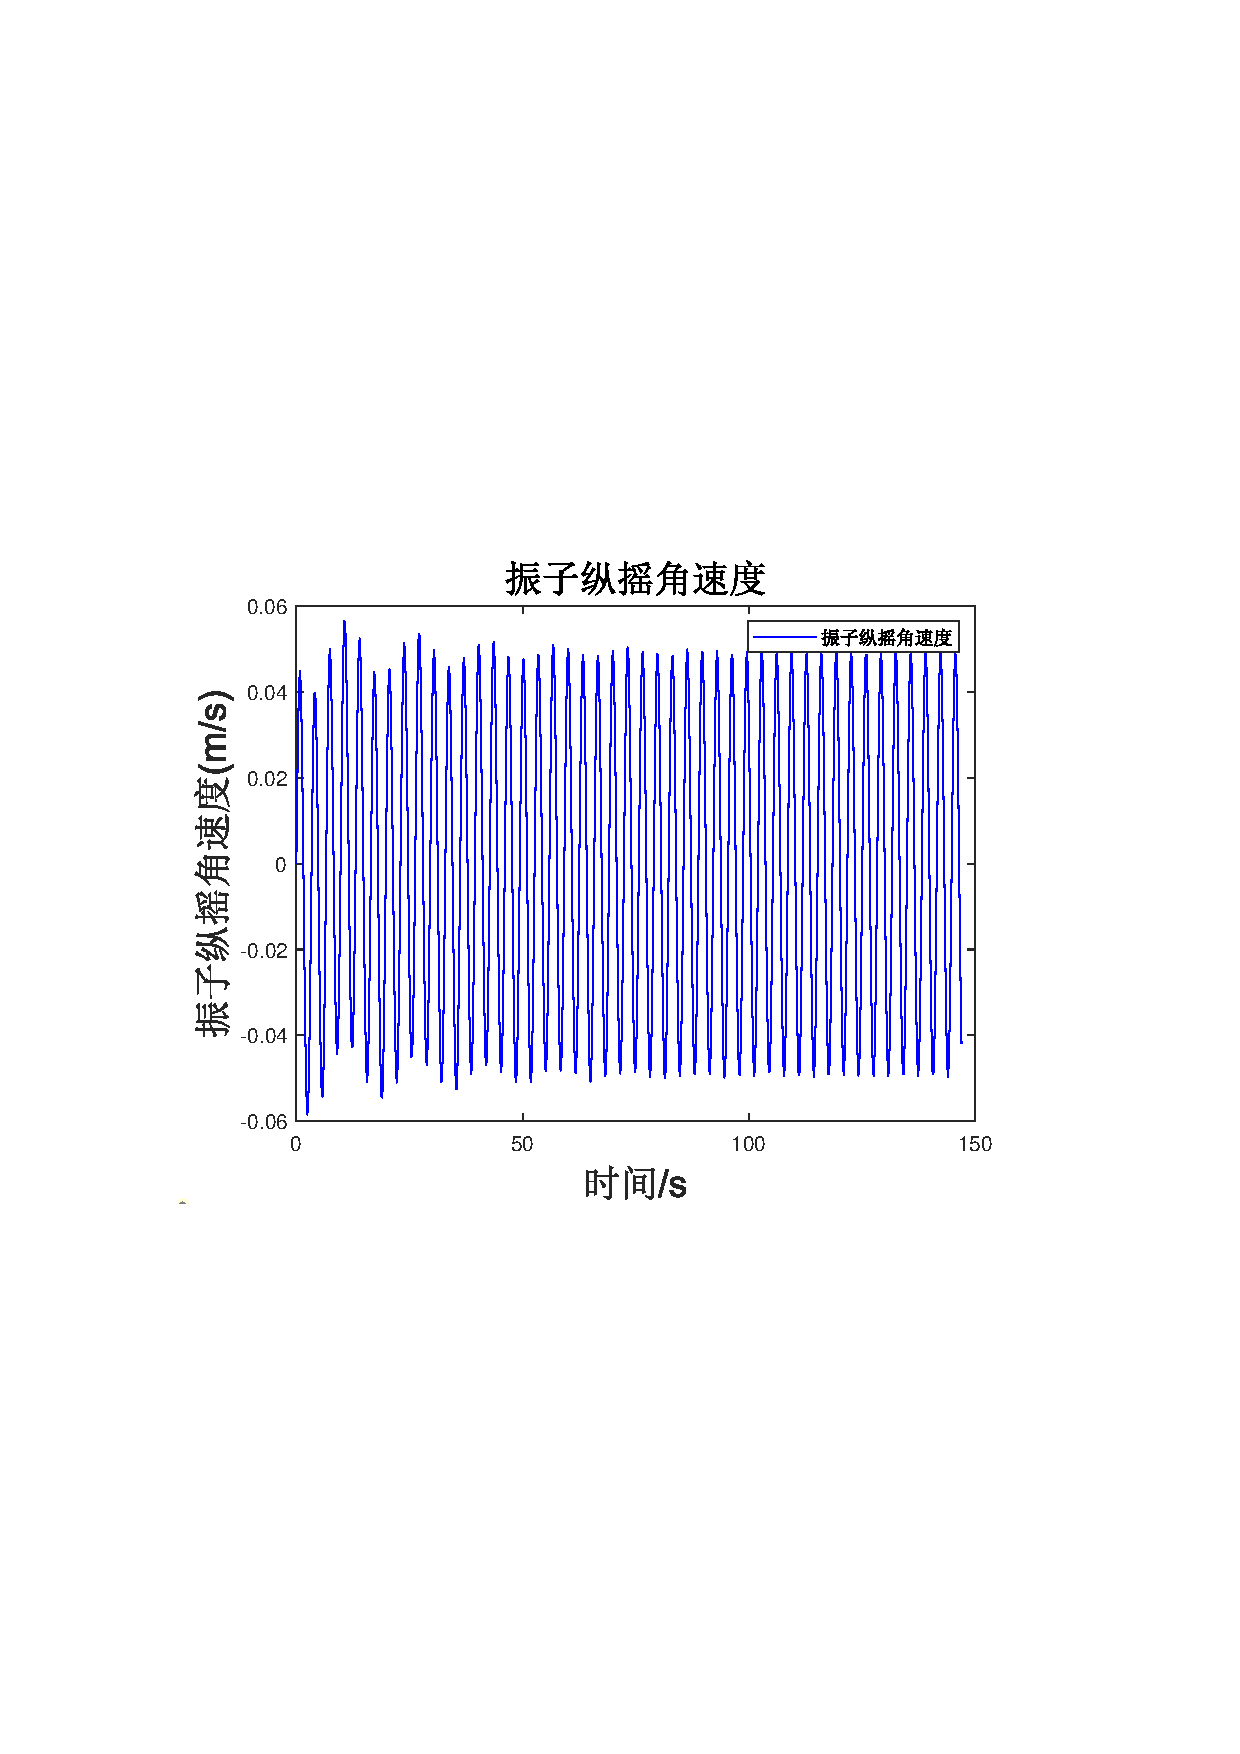
\includegraphics[width=0.9\linewidth]{figures/振子纵摇角速度.pdf}
	\end{minipage}
	\caption{浮子与振子垂荡与纵摇联合运动求解可视化展示}
\end{figure}




\subsection{问题4模型的建立与求解}

\subsubsection{模型的建立}

问题四的物理模型情境与问题三没有太大差别,我们可以基于问题三所建立的浮子-振子垂荡纵摇联合运动模型来求解问题四。问题四的主要探讨在特定直线阻尼系数和旋转阻尼系数情况下寻找最大化输出功率与对应的阻尼系数。因此,优化目标方程为浮子-振子垂荡纵摇联合运动模型中的输出功率函数。

基于先前对模型的分析,我们可以分别列出直线阻尼器输出功率与旋转阻尼器输出功率如下:
\begin{equation}
	\begin{cases}
		W_1 = \int_{t_0}^{t_1}K_z\dot{r}dr = \int_{t_0}^{t_1}K_z(\dot{r})^2dr \\
		W_2 = \int_{t_0}^{t_1} K_2\dot{\theta}d\theta = \int_{t_0}^{t_1}K_2(\theta)^2dt
	\end{cases}
\end{equation}

我们使用平均功率代表波浪能装置输出功率的能力,计算方法如下:
\begin{equation}
	P = \frac{W_1+W_2}{t_1-t_0}
\end{equation}

\subsubsection{模型的求解}

我们使用遗传算法对于输出功率进行优化。由于遗传算法具有一定的不确定性,我们进行了多次重复实验,所得到的最高结果为当旋转阻尼器阻尼系数为91132.8979、直线阻尼器阻尼系数为26977.6055时,所获得的最大功率为643.9142W。在此基础上为了得到更精确的解,我们在最优解范围内进行3D绘图,我们可以得到比初始解更为精确的最优解如图13所示。我们最终得出结论:

当旋转阻尼器阻尼系数为91149.5、直线阻尼器阻尼系数为26999.5时,波浪能装置获得最大平均输出功率644.024W。

\begin{figure}
	\centering
	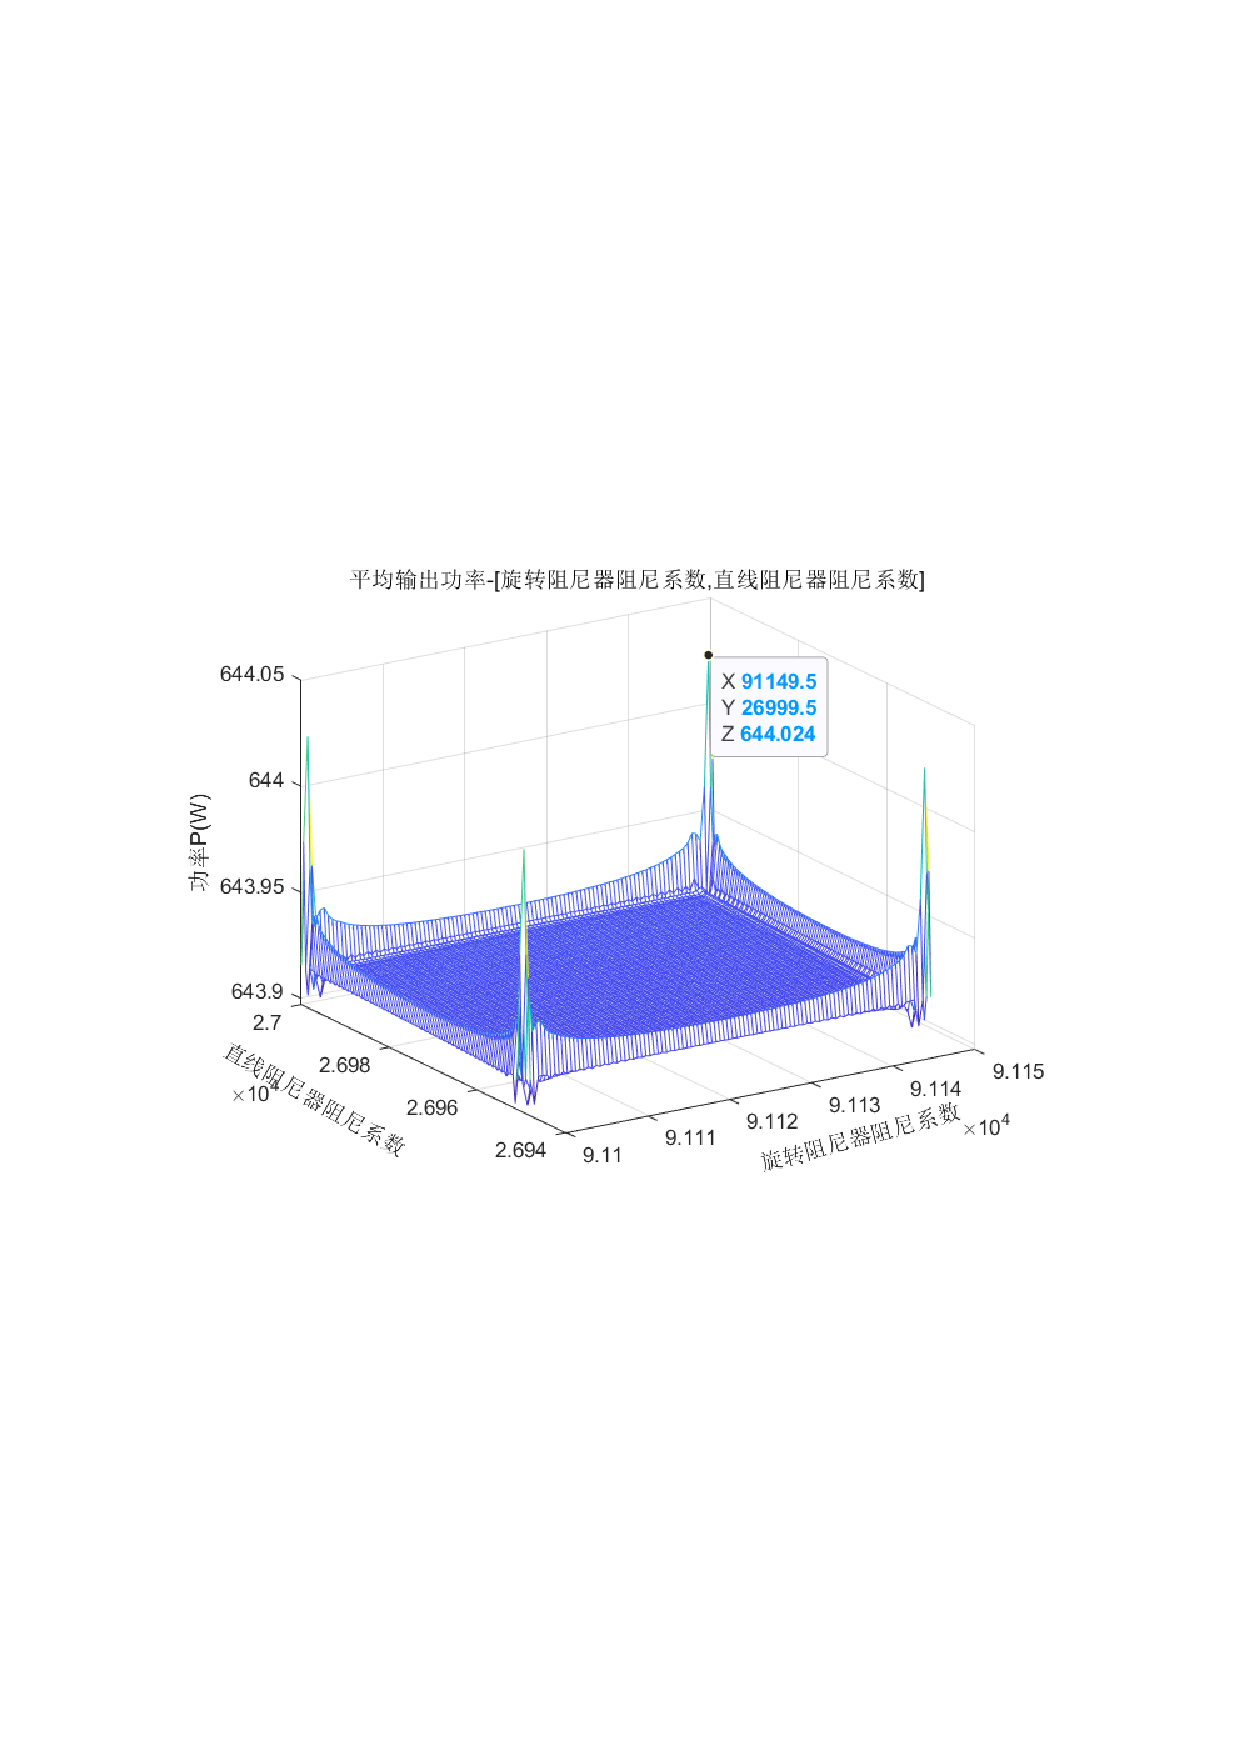
\includegraphics[width=0.7\linewidth]{figures/更为精确的最优解.pdf}
	\caption{问题四更为精确的最优解}
	\label{fig:}
\end{figure}



% chap 6
\section{模型的检验与误差分析/灵敏度分析}


\subsection{模型的检验}

首先我们验证模型的合理性。第一,我们认为系统能量来源在于波浪激励力对波浪能装置做功,因此预期是在不受外力的影响下,系统最终应当趋于稳定状态。我们对模型进行检验,在排除波浪激励力的作用下,波浪能装置的振荡幅度不断减小直至趋近于0(如图14所示),与预期相符,说明模型是合理的。

第二,我们认为在波浪激励力的作用下,系统稳定后,浮子的振动频率应和波浪激励力的振动频率一致。经过对模型的测试后,我们得出稳定后浮子和振子的垂荡频率为1.3998与题目波浪激励力频率1.4005十分接近。因此我们认为该模型具有一定的合理性。

接下来我们验证模型的鲁棒性。我们认为系统应当在一定输入范围内保持模型的一致性。经过对模型的测试,我们发现给定浮子一定范围内的不同初速度,浮子都能在一段时间后达到相同的稳定状态,在大部分情况下,模型在200s以内都能够实现结果的收敛。



\begin{figure}[htbp]
	\centering
	\subfloat[无波浪激励力浮子速度]{
		\begin{minipage}[t]{0.5\textwidth}
			\centering
			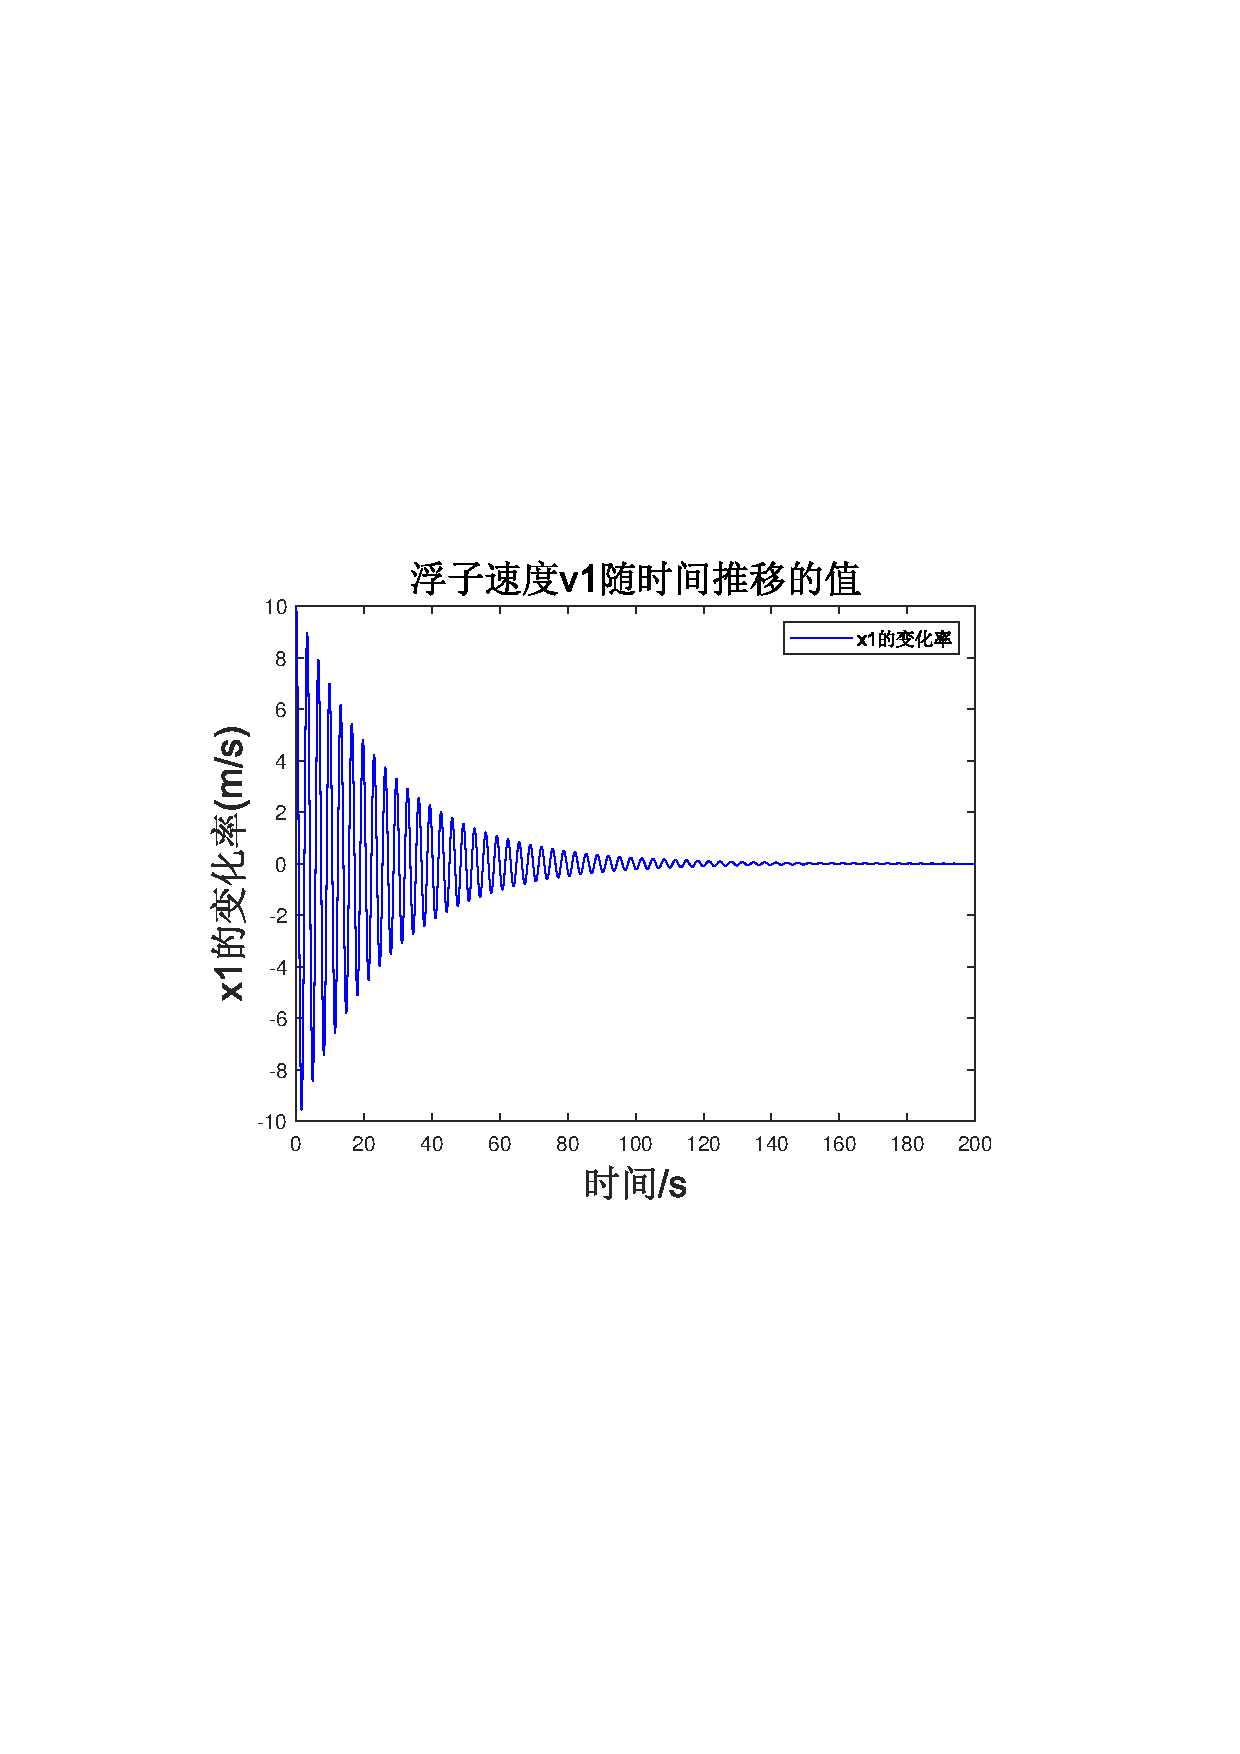
\includegraphics[width=0.8\linewidth]{figures/无波浪激励力浮子速度v1.pdf}
		\end{minipage}
	}
	\subfloat[无波浪激励力振子速度]{
		\begin{minipage}[t]{0.5\textwidth}
			\centering
			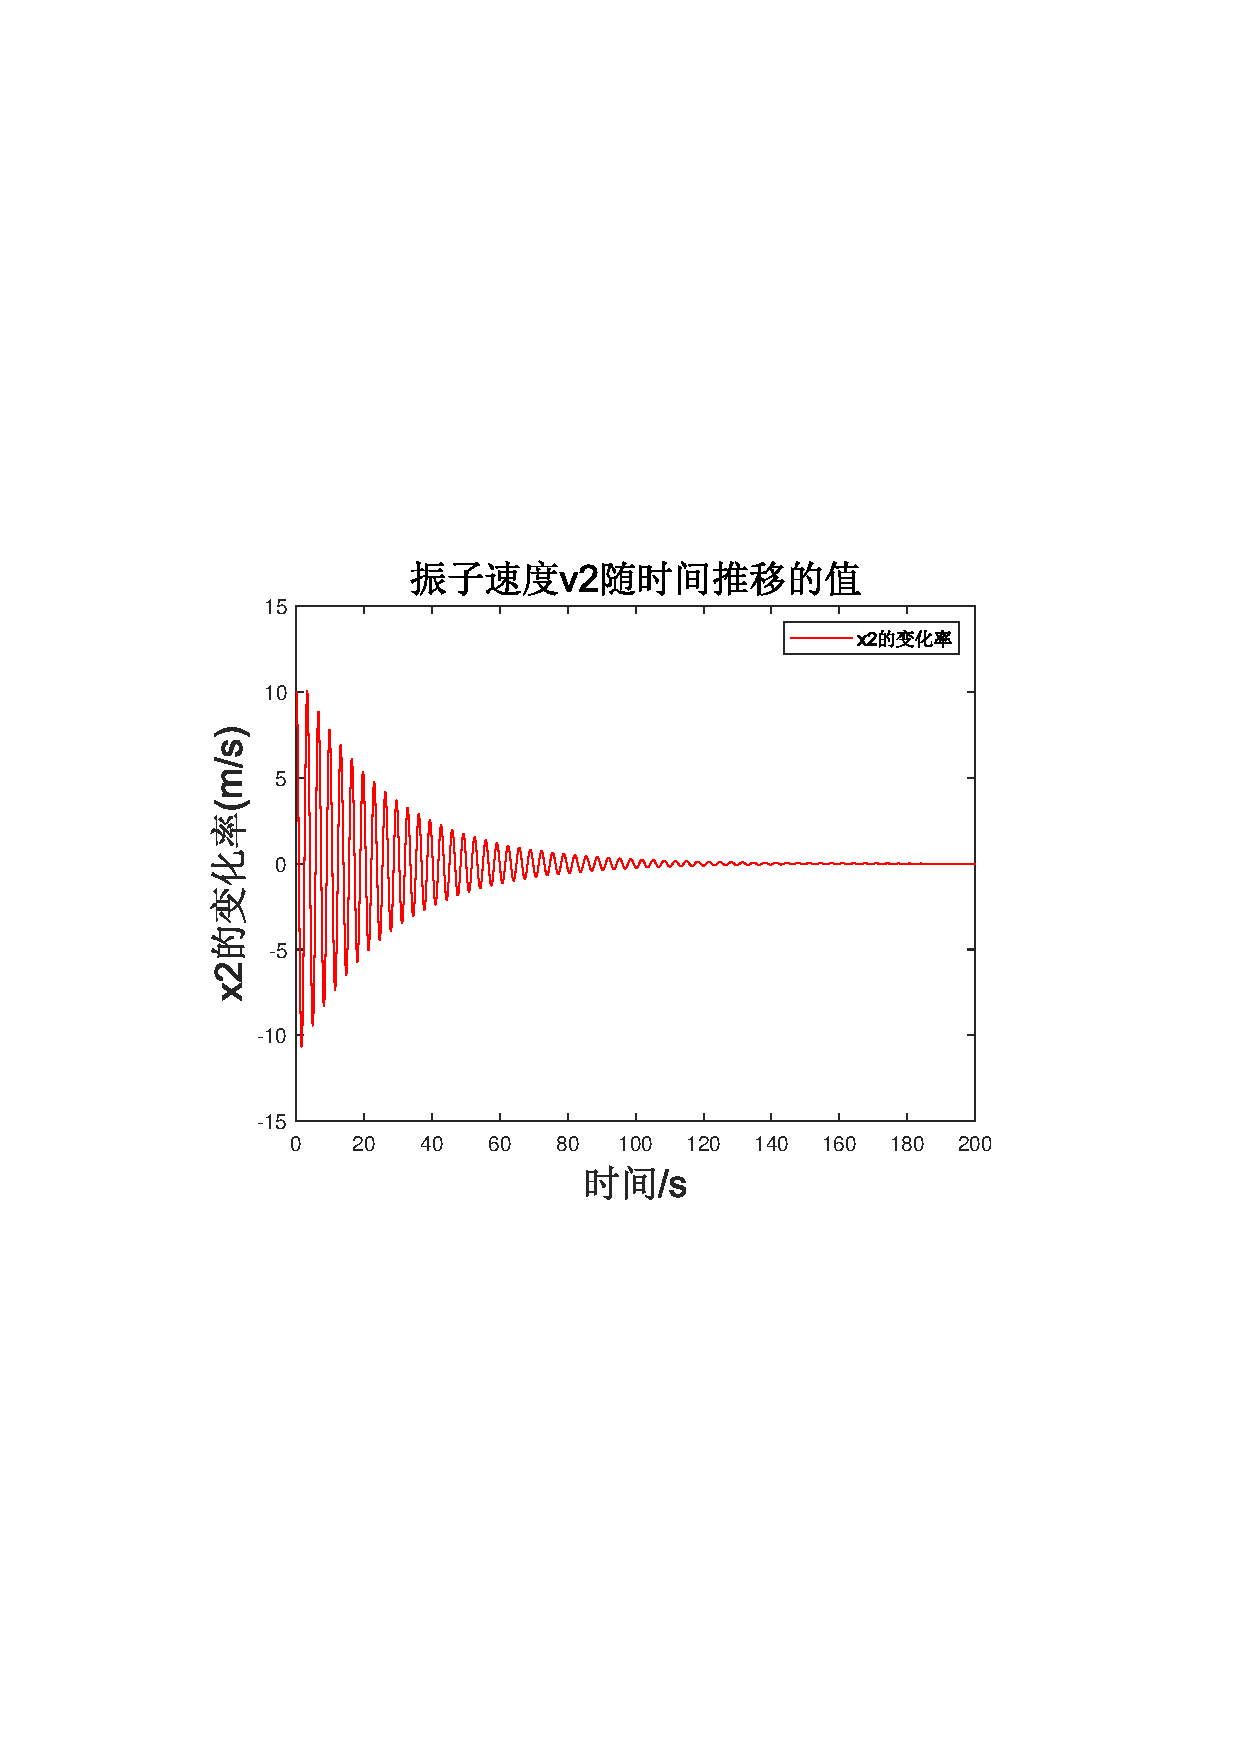
\includegraphics[width=0.8\linewidth]{figures/无波浪激励力振子速度v2.pdf}
		\end{minipage}
	}
	\caption{无波浪激励力作用}
\end{figure}

\begin{figure}
	\centering
	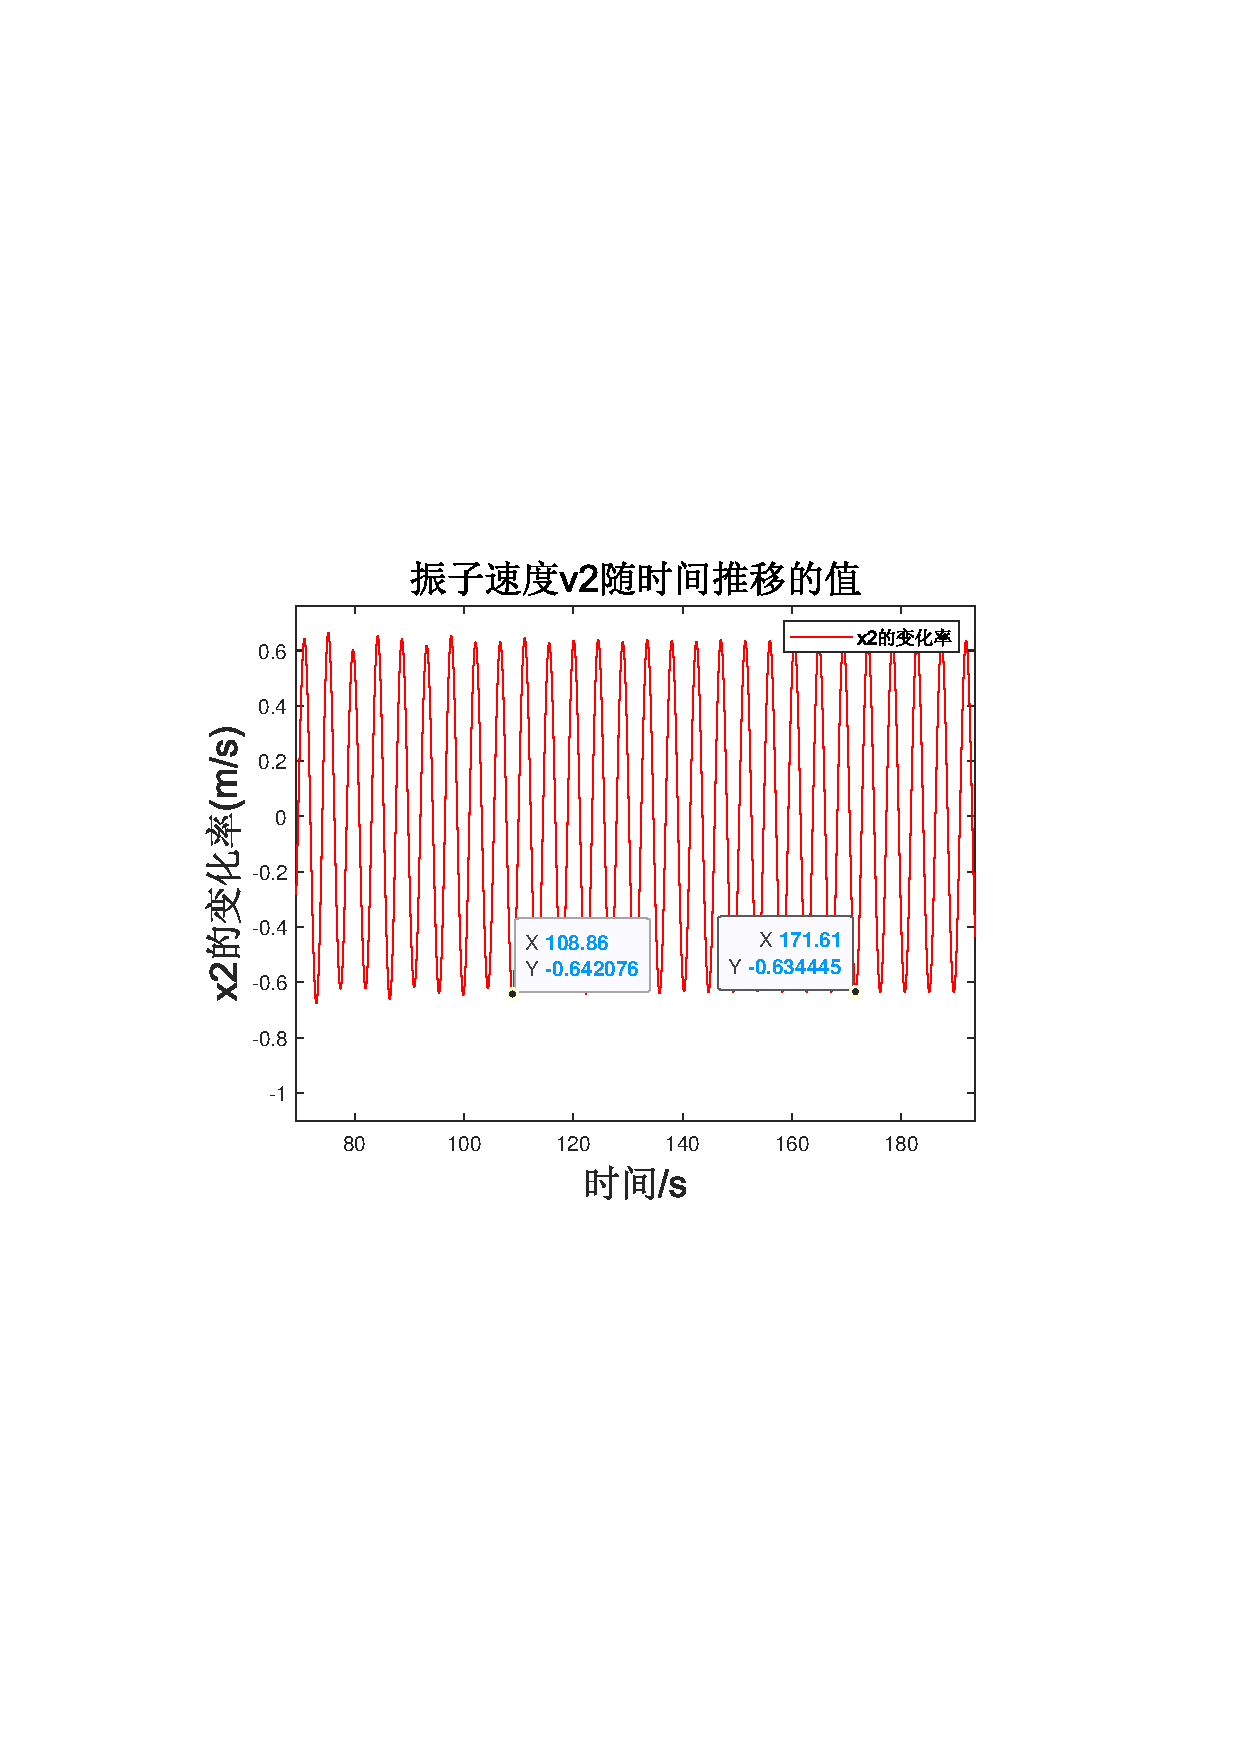
\includegraphics[width=0.7\linewidth]{figures/频率分析.pdf}
	\caption{频率分析}
\end{figure}

\subsection{误差分析}

经过充分讨论与分析,我们认为以下方面可能会对模型造成一定的误差:
\begin{enumerate}
	\item 为了简化对运动的分析,我们将浮子的运动分为o点的垂荡运动和浮子绕o点的转动,可能对运动状态的计算带来一定的误差;
	\item 忽略了浮子与振子的厚度,使得转动惯量的计算存在一定的误差;
	\item 忽略了在纵摇情况下波浪能装置重心偏移时装置重力力矩对静水恢复力矩的影响;
	\item 对于二阶常微分方程组的求解我们仅能求出数值解,存在一定的误差;
	\item 假定参与运动的对象全部为刚体,忽略了形变可能带来的影响;
\end{enumerate}




% chap 7
\section{模型的评价与推广}


\subsection{模型的评价}

\subsubsection{模型的优点}
\begin{enumerate}
\item 引入非惯性系和惯性力,使得系统的受力分析更为简单;
\item 在题目数据量较大的背景下,我们使用“二次计算法”进行快速优化求解,减少求得局部最优解的概率(第一次使用遗传算法对最优值进行初步求解,第二次通过绘制三维坐标图在第一次计算结果周围寻找更优解);
\item 我们基于牛顿运动定律对模型进行求解,易于理解,求解方便,且结果具有一定的合理性与准确性;
\end{enumerate}

\subsubsection{模型的缺点}

\begin{enumerate}
\item 该模型无法获得在任意情况下的解析解;
\item 该模型对于更加真实的海波情况无法运用牛顿运动定律进行求解;
\end{enumerate}

\subsection{模型的推广}
针对上述缺点,我们认为可以从以下几个方面进一步优化:
\begin{enumerate}
	\item 引入傅里叶变换与时域分析对运动状态函数进行更细致的刻画;
	\item 基于水动力学相关知识对水波与波浪能装置之间的相互作用进行更细致的描述;
\end{enumerate}
 
 
 
% chap 8
\newpage
\begin{thebibliography}{99}  
	\bibitem{ref1}崔琳,李蒙,白旭.海洋可再生能源技术现状与发展趋势[J].船舶工程,2021,43(10):22-33.
	
	\bibitem{ref2}尹冰涛.振荡浮子式波能提取装置的水动力学研究[D].浙江海洋大学,2021.DOI:10.27747/d.cnki.gzjhy.2021.000002.
	
	\bibitem{ref3}周衍柏 理论力学教程,高等教育出版社,1986. 
\end{thebibliography}

\clearpage

% chap 9
\section*{附录}

\appendix



\section{源程序}
 
\begin{lstlisting}[language=matlab,caption={求解问题1-1的MatLab代码}]
% 清空所有变量
clear
% 清空屏幕
clc

% 时间跨度取0-200,间隔为0.2
tspan = 0:0.2:200;
% 初始值
y0 = [0,0,0,0.2019];

% 调用语句
% ofn为直接算,offn为相对
[T,Y] = ode45( @offn, tspan, y0 );

% 绘图

% 浮子速度
figure(1);
plot(T,Y(:,1),'-b')
xlabel('时间/s','Fontsize',18);
ylabel('x1的变化率(m/s)','Fontsize',18);
title('浮子速度v1随时间推移的值','Fontsize',18)
legend('x1的变化率')

% 振子速度
figure(2);
plot(T,Y(:,1)+Y(:,2),'-r')
xlabel('时间/s','Fontsize',18);
ylabel('x2的变化率(m/s)','Fontsize',18);
title('振子速度v2随时间推移的值','Fontsize',18)
legend('x2的变化率')

% 浮子位移
figure(3);
plot(T,Y(:,3),'-b')
xlabel('时间/s','Fontsize',18);
ylabel('x1(m)','Fontsize',18);
title('浮子位移x1随时间推移的值','Fontsize',18)
legend('x1')

xx = Y(1,3) + Y(1,4) - 2;

% 振子位移
figure(4);
plot(T,Y(:,3)+Y(:,4)-2-xx,'-r')
xlabel('时间/s','Fontsize',18);
ylabel('x2(m)','Fontsize',18);
title('振子位移x2随时间推移的值','Fontsize',18)
legend('x2')
 \end{lstlisting}

\begin{lstlisting}[language=matlab,caption={求解问题1-2的MatLab代码}]
	% 清空所有变量
	clear
	% 清空屏幕
	clc
	
	% 时间跨度取0-200,间隔为0.2
	tspan = 0:0.2:200;
	% 初始值
	y0 = [0,0,0,0.2019];
	
	% 调用语句
	% ofn为直接算,offn为相对
	[T,Y] = ode45( @offn, tspan, y0 );
	
	% 绘图
	
	% 浮子速度
	figure(1);
	plot(T,Y(:,1),'-b')
	xlabel('时间/s','Fontsize',18);
	ylabel('x1的变化率(m/s)','Fontsize',18);
	title('浮子速度v1随时间推移的值','Fontsize',18)
	legend('x1的变化率')
	
	% 振子速度
	figure(2);
	plot(T,Y(:,1)+Y(:,2),'-r')
	xlabel('时间/s','Fontsize',18);
	ylabel('x2的变化率(m/s)','Fontsize',18);
	title('振子速度v2随时间推移的值','Fontsize',18)
	legend('x2的变化率')
	
	% 浮子位移
	figure(3);
	plot(T,Y(:,3),'-b')
	xlabel('时间/s','Fontsize',18);
	ylabel('x1(m)','Fontsize',18);
	title('浮子位移x1随时间推移的值','Fontsize',18)
	legend('x1')
	
	xx = Y(1,3) + Y(1,4) - 2;
	
	% 振子位移
	figure(4);
	plot(T,Y(:,4)+Y(:,3)-2-xx,'-r')
	xlabel('时间/s','Fontsize',18);
	ylabel('x2(m)','Fontsize',18);
	title('振子位移x2随时间推移的值','Fontsize',18)
	legend('x2')
	
	xlswrite('result1-2.xlsx',T,'A3:A903')
	xlswrite('result1-2.xlsx',Y(:,3),'B3:B903');
	xlswrite('result1-2.xlsx',Y(:,1),'C3:C903');
	xlswrite('result1-2.xlsx',Y(:,3)+Y(:,4)-2-xx,'D3:D903');
	xlswrite('result1-2.xlsx',Y(:,1)+Y(:,2),'E3:E903');
	
	fprintf("end\n")
 \end{lstlisting}

\begin{lstlisting}[language=matlab,caption={求解问题2-1的MatLab代码(粗算)}]
	% 清空所有变量
	clear
	% 清空屏幕
	clc
	
	% 时间跨度取0-200,间隔为0.01
	tspan = 0:0.01:200;
	
	% 初始值
	y0 = [0,0,0,0.2019];
	
	% 步长遍历
	% 粗
	k = 0:0.01:100000;
	
	% 结果存储
	res = [];
	
	% 积分的位置
	t0 = 40;
	t1 = 180;
	
	for i = 0:0.01:100000
	gb = i;
	% 调用语句
	% ofn为直接算,offn为相对
	[T,Y] = ode45( @(T,Y) offn(T,Y,gb), tspan, y0);
	
	% Y(:,2)
	
	R = 0;
	for j = t0:0.01:t1-0.01
	R = R + 0.005*gb*(power(Y(int16(j*100),2),2) ...
	+power(Y(int16(j*100+1),2),2));
	end
	
	res(end+1) = R/(t1-t0);
	
	%     fprintf("%.4f\n",R);
	% 
	fprintf("%d Done!\n",i);
	end
	
	[M,L] = max(res);
	
	fprintf("The max P is %.4f,the index is %d\n",M,I);
	
	% 绘图
	
	figure(1);
	plot(k,res,'-r');
	xlable('阻尼系数','Fontsize',18);
	ylable('输出功率/W','Fontsize',18);
	title('输出功率P随阻尼系数的增加的值','FontSize',18);
	legend('输出功率')
	
	fprintf("end\n")
\end{lstlisting}

\begin{lstlisting}[language=matlab,caption={求解问题2-1的MatLab代码(精算)}]
	% 清空所有变量
	clear
	% 清空屏幕
	clc
	
	% 时间跨度取0-200,间隔为0.01
	tspan = 0:0.01:200;
	
	% 初始值
	y0 = [0,0,0,0.2019];
	
	% 步长遍历
	% 粗
	% k = 0:1:100000;
	% 精
	k = 32000:0.01:33000;
	
	% 结果存储
	res = [];
	
	% 积分的位置
	t0 = 40;
	t1 = 180;
	
	for i = 31000:0.01:32000
	gb = i;
	% 调用语句
	% ofn为直接算,offn为相对
	[T,Y] = ode45( @(T,Y) offn(T,Y,gb), tspan, y0);
	
	% Y(:,2)
	
	R = 0;
	for j = t0:0.01:t1-0.01
	R = R + 0.005*gb*(power(Y(int16(j*100),2),2) ...
	+power(Y(int16(j*100+1),2),2));
	end
	
	res(end+1) = R/(t1-t0);
	
	%     fprintf("%.4f\n",R);
	% 
	fprintf("%d Done!\n",i);
	end
	
	[M,L] = max(res);
	
	fprintf("The max P is %.4f,the index is %d\n",M,I);
	
	% 绘图
	
	figure(1);
	plot(k,res,'-r');
	xlable('阻尼系数','Fontsize',18);
	ylable('输出功率/W','Fontsize',18);
	title('输出功率P随阻尼系数的增加的值','FontSize',18);
	legend('输出功率')
	
	% 相对速度
	% figure(4);
	% plot(T,Y(:,2),'-r')
	% xlabel('时间/s','Fontsize',18);
	% ylabel('y2(m/s)','Fontsize',18);
	% title('相对速度y2随时间推移的值','Fontsize',18)
	% legend('y2')
	
	fprintf("end\n")
\end{lstlisting}


\begin{lstlisting}[language=matlab,caption={求解问题2-2的MatLab代码}]
	% 清空所有变量
	clear
	% 清空屏幕
	clc
	
	lb = [0;0];
	ub = [100000;1];
	
	res = [];
	
	for i = 1:10
	
	tic
	x = ga(@tar,2,[],[],[],[],lb,ub);
	-tar(x);
	toc
	
	fprintf("The gb is %.4f\tThe gk is %.4f\n",x(1),x(2));
	
	% 积分的位置
	t0 = 150;
	t1 = 190;
	
	% 时间跨度取0-200,间隔为0.01
	tspan = 0:0.01:200;
	
	% 初始值
	y0 = [0,0,0,0.2019];
	
	[~,Y] = ode45( @(T,Y) offn(T,Y,x(1),x(2)), tspan, y0);
	
	R = 0;
	for j = t0:0.01:t1-0.01
	R = R + 0.005*x(1)*(power(abs(Y(int16(j*100),2)),2+x(2)) ...
	+power(abs(Y(int16(j*100+1),2)),2+x(2)));
	end
	
	res = [res [x(1) x(2) R / (t1-t0)]];
	
	fprintf("The index of %d has done!\n",i)
	
	end
	
	fprintf("end\n")
\end{lstlisting}

\begin{lstlisting}[language=matlab,caption={求解问题3的MatLab代码}]
	% 清空所有变量
	clear
	% 清空屏幕
	clc
	
	% 时间跨度取0-200,间隔为0.2
	tspan = 0:0.2:147;
	% 初始值
	y0 = [0,0,0,0,0,0,0,0.2019];
	
	% 调用语句
	% ofn为直接算,offn为相对
	[T,Y] = ode45( @offn11, tspan, y0 );
	X=Y(:,7);   %浮子垂荡位移
	X1=Y(:,3);  %浮子垂荡速度
	A=Y(:,5);   %浮子纵摇角位移
	A1=Y(:,1);   %浮子纵摇角速度
	R=Y(:,8);    %振子相对浮子径向位移
	R1=Y(:,4);    %振子相对浮子径向速度
	B=Y(:,6);    %振子相对浮子角位移
	B1=Y(:,2);   %振子相对浮子角速度
	
	Z=X+R.*cos(A+B)-0.2019;  %振子的垂荡位移
	Z1=X1+R1.*cos(A+B)-R.*sin(A+B).*(A1+B1); %振子的纵摇速度
	C=A+B;           %振子的纵摇角位移
	C1=A1+B1;        %振子的纵摇角速度
	
	% % 浮子角速度
	figure(1);
	plot(T,Y(:,1),'-b')
	xlabel('时间/s','Fontsize',18);
	ylabel('浮子的角速度(rad/s)','Fontsize',18);
	title('浮子角速度','Fontsize',18)
	legend('浮子的角速度')
	
	%振子相对浮子的角速度
	% figure(2);
	% plot(T,Y(:,2),'-b')
	% xlabel('时间/s','Fontsize',18);
	% ylabel('振子相对浮子的角速度(rad/s)','Fontsize',18);
	% title('振子相对浮子的角速度','Fontsize',18)
	% legend('振子相对浮子的角速度')
	
	%浮子的垂荡速度
	figure(3);
	plot(T,Y(:,3),'-b')
	xlabel('时间/s','Fontsize',18);
	ylabel('浮子的垂荡速度(m/s)','Fontsize',18);
	title('浮子的垂荡速度','Fontsize',18)
	legend('浮子的垂荡速度')
	
	%振子相对浮子的径向速度
	% figure(4);
	% plot(T,Y(:,4),'-b')
	% xlabel('时间/s','Fontsize',18);
	% ylabel('振子相对浮子的径向速度(m/s)','Fontsize',18);
	% title('振子相对浮子的径向速度','Fontsize',18)
	% legend('振子相对浮子的径向速度')
	
	%浮子的角位移
	figure(5);
	plot(T,Y(:,5),'-b')
	xlabel('时间/s','Fontsize',18);
	ylabel('浮子的角位移(rad)','Fontsize',18);
	title('浮子的角位移','Fontsize',18)
	legend('浮子的角位移')
	
	%振子相对浮子的角位移
	% figure(6);
	% plot(T,Y(:,6),'-b')
	% xlabel('时间/s','Fontsize',18);
	% ylabel('振子相对浮子的角位移(rad)','Fontsize',18);
	% title('振子相对浮子的角位移','Fontsize',18)
	% legend('振子相对浮子的角位移')
	
	%浮子的垂荡位移
	figure(7);
	plot(T,Y(:,7),'-b')
	xlabel('时间/s','Fontsize',18);
	ylabel('浮子的垂荡位移(m)','Fontsize',18);
	title('浮子的垂荡位移','Fontsize',18)
	legend('浮子的垂荡位移')
	
	%振子相对浮子的径向位移
	% figure(8);
	% plot(T,Y(:,8),'-b')
	% xlabel('时间/s','Fontsize',18);
	% ylabel('振子相对浮子的径向位移(m)','Fontsize',18);
	% title('振子相对浮子的径向位移','Fontsize',18)
	% legend('振子相对浮子的径向位移')
	
	%振子垂荡位移
	figure(9);
	plot(T,Z,'-b')
	xlabel('时间/s','Fontsize',18);
	ylabel('振子垂荡位移(m)','Fontsize',18);
	title('振子垂荡位移','Fontsize',18)
	legend('振子垂荡位移')
	
	%振子垂荡速度
	figure(10);
	plot(T,Z1,'-b')
	xlabel('时间/s','Fontsize',18);
	ylabel('振子垂荡速度(m/s)','Fontsize',18);
	title('振子垂荡速度','Fontsize',18)
	legend('振子垂荡速度')
	
	%振子纵摇角位移
	figure(11);
	plot(T,C,'-b')
	xlabel('时间/s','Fontsize',18);
	ylabel('振子纵摇角位移(m)','Fontsize',18);
	title('振子纵摇角位移','Fontsize',18)
	legend('振子纵摇角位移')
	
	%振子纵摇角速度
	figure(12);
	plot(T,C1,'-b')
	xlabel('时间/s','Fontsize',18);
	ylabel('振子纵摇角速度(m/s)','Fontsize',18);
	title('振子纵摇角速度','Fontsize',18)
	legend('振子纵摇角速度')
\end{lstlisting}

\begin{lstlisting}[language=matlab,caption={求解问题4的MatLab代码}]
	% 清空所有变量
	clear
	% 清空屏幕
	clc
	
	lb = [0;0];
	ub = [100000;100000];
	
	res = [];
	
	% 求十次取最优
	for i = 1:1:10
	
	tic
	x = ga(@tar,2,[],[],[],[],lb,ub);
	-tar(x);
	toc
	
	fprintf("The gb is %.4f\tThe gk is %.4f\n",x(1),x(2));
	
	% 时间跨度取0-200,间隔为0.01
	tspan = 0:0.01:200;
	
	% 初始值
	y0 = [0,0,0,0,0,0,0,0.2019];
	
	[~,Y] = ode45( @(T,Y) offn(T,Y,x(1),x(2)), tspan, y0);
	
	% 积分的位置
	t0 = 150;
	t1 = 190;
	
	R1 = 0;
	R2 = 0;
	for j = t0:0.01:t1-0.01
	R1 = R1 + 0.005*x(1)*(power(abs(Y(int16(j*100),2)),2) ...
	+power(abs(Y(int16(j*100+1),2)),2));
	R2 = R2 + 0.005*x(2)*(power(abs(Y(int16(j*100),4)),2) ...
	+power(abs(Y(int16(j*100+1),4)),2));
	end
	
	R = (R1+R2)/(t1-t0);
	
	res = [res [x(1) x(2) R]];
	
	end
	
	res = reshape(res,3,10);
	
	x = res(1,:);
	y = res(2,:);
	z = res(3,:);
	
	xlswrite('best.xlsx',x,'A1:I1');
	xlswrite('best.xlsx',y,'A2:I2');
	xlswrite('best.xlsx',z,'A3:I3');
	
	fprintf("end\n")
\end{lstlisting}

\end{document}